
% Default to the notebook output style

    


% Inherit from the specified cell style.




    
\documentclass[11pt]{article}

    
    
    \usepackage[T1]{fontenc}
    % Nicer default font (+ math font) than Computer Modern for most use cases
    \usepackage{mathpazo}

    % Basic figure setup, for now with no caption control since it's done
    % automatically by Pandoc (which extracts ![](path) syntax from Markdown).
    \usepackage{graphicx}
    % We will generate all images so they have a width \maxwidth. This means
    % that they will get their normal width if they fit onto the page, but
    % are scaled down if they would overflow the margins.
    \makeatletter
    \def\maxwidth{\ifdim\Gin@nat@width>\linewidth\linewidth
    \else\Gin@nat@width\fi}
    \makeatother
    \let\Oldincludegraphics\includegraphics
    % Set max figure width to be 80% of text width, for now hardcoded.
    \renewcommand{\includegraphics}[1]{\Oldincludegraphics[width=.8\maxwidth]{#1}}
    % Ensure that by default, figures have no caption (until we provide a
    % proper Figure object with a Caption API and a way to capture that
    % in the conversion process - todo).
    \usepackage{caption}
    \DeclareCaptionLabelFormat{nolabel}{}
    \captionsetup{labelformat=nolabel}

    \usepackage{adjustbox} % Used to constrain images to a maximum size 
    \usepackage{xcolor} % Allow colors to be defined
    \usepackage{enumerate} % Needed for markdown enumerations to work
    \usepackage{geometry} % Used to adjust the document margins
    \usepackage{amsmath} % Equations
    \usepackage{amssymb} % Equations
    \usepackage{textcomp} % defines textquotesingle
    % Hack from http://tex.stackexchange.com/a/47451/13684:
    \AtBeginDocument{%
        \def\PYZsq{\textquotesingle}% Upright quotes in Pygmentized code
    }
    \usepackage{upquote} % Upright quotes for verbatim code
    \usepackage{eurosym} % defines \euro
    \usepackage[mathletters]{ucs} % Extended unicode (utf-8) support
    \usepackage[utf8x]{inputenc} % Allow utf-8 characters in the tex document
    \usepackage{fancyvrb} % verbatim replacement that allows latex
    \usepackage{grffile} % extends the file name processing of package graphics 
                         % to support a larger range 
    % The hyperref package gives us a pdf with properly built
    % internal navigation ('pdf bookmarks' for the table of contents,
    % internal cross-reference links, web links for URLs, etc.)
    \usepackage{hyperref}
    \usepackage{longtable} % longtable support required by pandoc >1.10
    \usepackage{booktabs}  % table support for pandoc > 1.12.2
    \usepackage[inline]{enumitem} % IRkernel/repr support (it uses the enumerate* environment)
    \usepackage[normalem]{ulem} % ulem is needed to support strikethroughs (\sout)
                                % normalem makes italics be italics, not underlines
    

    
    
    % Colors for the hyperref package
    \definecolor{urlcolor}{rgb}{0,.145,.698}
    \definecolor{linkcolor}{rgb}{.71,0.21,0.01}
    \definecolor{citecolor}{rgb}{.12,.54,.11}

    % ANSI colors
    \definecolor{ansi-black}{HTML}{3E424D}
    \definecolor{ansi-black-intense}{HTML}{282C36}
    \definecolor{ansi-red}{HTML}{E75C58}
    \definecolor{ansi-red-intense}{HTML}{B22B31}
    \definecolor{ansi-green}{HTML}{00A250}
    \definecolor{ansi-green-intense}{HTML}{007427}
    \definecolor{ansi-yellow}{HTML}{DDB62B}
    \definecolor{ansi-yellow-intense}{HTML}{B27D12}
    \definecolor{ansi-blue}{HTML}{208FFB}
    \definecolor{ansi-blue-intense}{HTML}{0065CA}
    \definecolor{ansi-magenta}{HTML}{D160C4}
    \definecolor{ansi-magenta-intense}{HTML}{A03196}
    \definecolor{ansi-cyan}{HTML}{60C6C8}
    \definecolor{ansi-cyan-intense}{HTML}{258F8F}
    \definecolor{ansi-white}{HTML}{C5C1B4}
    \definecolor{ansi-white-intense}{HTML}{A1A6B2}

    % commands and environments needed by pandoc snippets
    % extracted from the output of `pandoc -s`
    \providecommand{\tightlist}{%
      \setlength{\itemsep}{0pt}\setlength{\parskip}{0pt}}
    \DefineVerbatimEnvironment{Highlighting}{Verbatim}{commandchars=\\\{\}}
    % Add ',fontsize=\small' for more characters per line
    \newenvironment{Shaded}{}{}
    \newcommand{\KeywordTok}[1]{\textcolor[rgb]{0.00,0.44,0.13}{\textbf{{#1}}}}
    \newcommand{\DataTypeTok}[1]{\textcolor[rgb]{0.56,0.13,0.00}{{#1}}}
    \newcommand{\DecValTok}[1]{\textcolor[rgb]{0.25,0.63,0.44}{{#1}}}
    \newcommand{\BaseNTok}[1]{\textcolor[rgb]{0.25,0.63,0.44}{{#1}}}
    \newcommand{\FloatTok}[1]{\textcolor[rgb]{0.25,0.63,0.44}{{#1}}}
    \newcommand{\CharTok}[1]{\textcolor[rgb]{0.25,0.44,0.63}{{#1}}}
    \newcommand{\StringTok}[1]{\textcolor[rgb]{0.25,0.44,0.63}{{#1}}}
    \newcommand{\CommentTok}[1]{\textcolor[rgb]{0.38,0.63,0.69}{\textit{{#1}}}}
    \newcommand{\OtherTok}[1]{\textcolor[rgb]{0.00,0.44,0.13}{{#1}}}
    \newcommand{\AlertTok}[1]{\textcolor[rgb]{1.00,0.00,0.00}{\textbf{{#1}}}}
    \newcommand{\FunctionTok}[1]{\textcolor[rgb]{0.02,0.16,0.49}{{#1}}}
    \newcommand{\RegionMarkerTok}[1]{{#1}}
    \newcommand{\ErrorTok}[1]{\textcolor[rgb]{1.00,0.00,0.00}{\textbf{{#1}}}}
    \newcommand{\NormalTok}[1]{{#1}}
    
    % Additional commands for more recent versions of Pandoc
    \newcommand{\ConstantTok}[1]{\textcolor[rgb]{0.53,0.00,0.00}{{#1}}}
    \newcommand{\SpecialCharTok}[1]{\textcolor[rgb]{0.25,0.44,0.63}{{#1}}}
    \newcommand{\VerbatimStringTok}[1]{\textcolor[rgb]{0.25,0.44,0.63}{{#1}}}
    \newcommand{\SpecialStringTok}[1]{\textcolor[rgb]{0.73,0.40,0.53}{{#1}}}
    \newcommand{\ImportTok}[1]{{#1}}
    \newcommand{\DocumentationTok}[1]{\textcolor[rgb]{0.73,0.13,0.13}{\textit{{#1}}}}
    \newcommand{\AnnotationTok}[1]{\textcolor[rgb]{0.38,0.63,0.69}{\textbf{\textit{{#1}}}}}
    \newcommand{\CommentVarTok}[1]{\textcolor[rgb]{0.38,0.63,0.69}{\textbf{\textit{{#1}}}}}
    \newcommand{\VariableTok}[1]{\textcolor[rgb]{0.10,0.09,0.49}{{#1}}}
    \newcommand{\ControlFlowTok}[1]{\textcolor[rgb]{0.00,0.44,0.13}{\textbf{{#1}}}}
    \newcommand{\OperatorTok}[1]{\textcolor[rgb]{0.40,0.40,0.40}{{#1}}}
    \newcommand{\BuiltInTok}[1]{{#1}}
    \newcommand{\ExtensionTok}[1]{{#1}}
    \newcommand{\PreprocessorTok}[1]{\textcolor[rgb]{0.74,0.48,0.00}{{#1}}}
    \newcommand{\AttributeTok}[1]{\textcolor[rgb]{0.49,0.56,0.16}{{#1}}}
    \newcommand{\InformationTok}[1]{\textcolor[rgb]{0.38,0.63,0.69}{\textbf{\textit{{#1}}}}}
    \newcommand{\WarningTok}[1]{\textcolor[rgb]{0.38,0.63,0.69}{\textbf{\textit{{#1}}}}}
    
    
    % Define a nice break command that doesn't care if a line doesn't already
    % exist.
    \def\br{\hspace*{\fill} \\* }
    % Math Jax compatability definitions
    \def\gt{>}
    \def\lt{<}
    % Document parameters
    \title{airbnb\_challenge\_submission}
    
    
    

    % Pygments definitions
    
\makeatletter
\def\PY@reset{\let\PY@it=\relax \let\PY@bf=\relax%
    \let\PY@ul=\relax \let\PY@tc=\relax%
    \let\PY@bc=\relax \let\PY@ff=\relax}
\def\PY@tok#1{\csname PY@tok@#1\endcsname}
\def\PY@toks#1+{\ifx\relax#1\empty\else%
    \PY@tok{#1}\expandafter\PY@toks\fi}
\def\PY@do#1{\PY@bc{\PY@tc{\PY@ul{%
    \PY@it{\PY@bf{\PY@ff{#1}}}}}}}
\def\PY#1#2{\PY@reset\PY@toks#1+\relax+\PY@do{#2}}

\expandafter\def\csname PY@tok@w\endcsname{\def\PY@tc##1{\textcolor[rgb]{0.73,0.73,0.73}{##1}}}
\expandafter\def\csname PY@tok@c\endcsname{\let\PY@it=\textit\def\PY@tc##1{\textcolor[rgb]{0.25,0.50,0.50}{##1}}}
\expandafter\def\csname PY@tok@cp\endcsname{\def\PY@tc##1{\textcolor[rgb]{0.74,0.48,0.00}{##1}}}
\expandafter\def\csname PY@tok@k\endcsname{\let\PY@bf=\textbf\def\PY@tc##1{\textcolor[rgb]{0.00,0.50,0.00}{##1}}}
\expandafter\def\csname PY@tok@kp\endcsname{\def\PY@tc##1{\textcolor[rgb]{0.00,0.50,0.00}{##1}}}
\expandafter\def\csname PY@tok@kt\endcsname{\def\PY@tc##1{\textcolor[rgb]{0.69,0.00,0.25}{##1}}}
\expandafter\def\csname PY@tok@o\endcsname{\def\PY@tc##1{\textcolor[rgb]{0.40,0.40,0.40}{##1}}}
\expandafter\def\csname PY@tok@ow\endcsname{\let\PY@bf=\textbf\def\PY@tc##1{\textcolor[rgb]{0.67,0.13,1.00}{##1}}}
\expandafter\def\csname PY@tok@nb\endcsname{\def\PY@tc##1{\textcolor[rgb]{0.00,0.50,0.00}{##1}}}
\expandafter\def\csname PY@tok@nf\endcsname{\def\PY@tc##1{\textcolor[rgb]{0.00,0.00,1.00}{##1}}}
\expandafter\def\csname PY@tok@nc\endcsname{\let\PY@bf=\textbf\def\PY@tc##1{\textcolor[rgb]{0.00,0.00,1.00}{##1}}}
\expandafter\def\csname PY@tok@nn\endcsname{\let\PY@bf=\textbf\def\PY@tc##1{\textcolor[rgb]{0.00,0.00,1.00}{##1}}}
\expandafter\def\csname PY@tok@ne\endcsname{\let\PY@bf=\textbf\def\PY@tc##1{\textcolor[rgb]{0.82,0.25,0.23}{##1}}}
\expandafter\def\csname PY@tok@nv\endcsname{\def\PY@tc##1{\textcolor[rgb]{0.10,0.09,0.49}{##1}}}
\expandafter\def\csname PY@tok@no\endcsname{\def\PY@tc##1{\textcolor[rgb]{0.53,0.00,0.00}{##1}}}
\expandafter\def\csname PY@tok@nl\endcsname{\def\PY@tc##1{\textcolor[rgb]{0.63,0.63,0.00}{##1}}}
\expandafter\def\csname PY@tok@ni\endcsname{\let\PY@bf=\textbf\def\PY@tc##1{\textcolor[rgb]{0.60,0.60,0.60}{##1}}}
\expandafter\def\csname PY@tok@na\endcsname{\def\PY@tc##1{\textcolor[rgb]{0.49,0.56,0.16}{##1}}}
\expandafter\def\csname PY@tok@nt\endcsname{\let\PY@bf=\textbf\def\PY@tc##1{\textcolor[rgb]{0.00,0.50,0.00}{##1}}}
\expandafter\def\csname PY@tok@nd\endcsname{\def\PY@tc##1{\textcolor[rgb]{0.67,0.13,1.00}{##1}}}
\expandafter\def\csname PY@tok@s\endcsname{\def\PY@tc##1{\textcolor[rgb]{0.73,0.13,0.13}{##1}}}
\expandafter\def\csname PY@tok@sd\endcsname{\let\PY@it=\textit\def\PY@tc##1{\textcolor[rgb]{0.73,0.13,0.13}{##1}}}
\expandafter\def\csname PY@tok@si\endcsname{\let\PY@bf=\textbf\def\PY@tc##1{\textcolor[rgb]{0.73,0.40,0.53}{##1}}}
\expandafter\def\csname PY@tok@se\endcsname{\let\PY@bf=\textbf\def\PY@tc##1{\textcolor[rgb]{0.73,0.40,0.13}{##1}}}
\expandafter\def\csname PY@tok@sr\endcsname{\def\PY@tc##1{\textcolor[rgb]{0.73,0.40,0.53}{##1}}}
\expandafter\def\csname PY@tok@ss\endcsname{\def\PY@tc##1{\textcolor[rgb]{0.10,0.09,0.49}{##1}}}
\expandafter\def\csname PY@tok@sx\endcsname{\def\PY@tc##1{\textcolor[rgb]{0.00,0.50,0.00}{##1}}}
\expandafter\def\csname PY@tok@m\endcsname{\def\PY@tc##1{\textcolor[rgb]{0.40,0.40,0.40}{##1}}}
\expandafter\def\csname PY@tok@gh\endcsname{\let\PY@bf=\textbf\def\PY@tc##1{\textcolor[rgb]{0.00,0.00,0.50}{##1}}}
\expandafter\def\csname PY@tok@gu\endcsname{\let\PY@bf=\textbf\def\PY@tc##1{\textcolor[rgb]{0.50,0.00,0.50}{##1}}}
\expandafter\def\csname PY@tok@gd\endcsname{\def\PY@tc##1{\textcolor[rgb]{0.63,0.00,0.00}{##1}}}
\expandafter\def\csname PY@tok@gi\endcsname{\def\PY@tc##1{\textcolor[rgb]{0.00,0.63,0.00}{##1}}}
\expandafter\def\csname PY@tok@gr\endcsname{\def\PY@tc##1{\textcolor[rgb]{1.00,0.00,0.00}{##1}}}
\expandafter\def\csname PY@tok@ge\endcsname{\let\PY@it=\textit}
\expandafter\def\csname PY@tok@gs\endcsname{\let\PY@bf=\textbf}
\expandafter\def\csname PY@tok@gp\endcsname{\let\PY@bf=\textbf\def\PY@tc##1{\textcolor[rgb]{0.00,0.00,0.50}{##1}}}
\expandafter\def\csname PY@tok@go\endcsname{\def\PY@tc##1{\textcolor[rgb]{0.53,0.53,0.53}{##1}}}
\expandafter\def\csname PY@tok@gt\endcsname{\def\PY@tc##1{\textcolor[rgb]{0.00,0.27,0.87}{##1}}}
\expandafter\def\csname PY@tok@err\endcsname{\def\PY@bc##1{\setlength{\fboxsep}{0pt}\fcolorbox[rgb]{1.00,0.00,0.00}{1,1,1}{\strut ##1}}}
\expandafter\def\csname PY@tok@kc\endcsname{\let\PY@bf=\textbf\def\PY@tc##1{\textcolor[rgb]{0.00,0.50,0.00}{##1}}}
\expandafter\def\csname PY@tok@kd\endcsname{\let\PY@bf=\textbf\def\PY@tc##1{\textcolor[rgb]{0.00,0.50,0.00}{##1}}}
\expandafter\def\csname PY@tok@kn\endcsname{\let\PY@bf=\textbf\def\PY@tc##1{\textcolor[rgb]{0.00,0.50,0.00}{##1}}}
\expandafter\def\csname PY@tok@kr\endcsname{\let\PY@bf=\textbf\def\PY@tc##1{\textcolor[rgb]{0.00,0.50,0.00}{##1}}}
\expandafter\def\csname PY@tok@bp\endcsname{\def\PY@tc##1{\textcolor[rgb]{0.00,0.50,0.00}{##1}}}
\expandafter\def\csname PY@tok@fm\endcsname{\def\PY@tc##1{\textcolor[rgb]{0.00,0.00,1.00}{##1}}}
\expandafter\def\csname PY@tok@vc\endcsname{\def\PY@tc##1{\textcolor[rgb]{0.10,0.09,0.49}{##1}}}
\expandafter\def\csname PY@tok@vg\endcsname{\def\PY@tc##1{\textcolor[rgb]{0.10,0.09,0.49}{##1}}}
\expandafter\def\csname PY@tok@vi\endcsname{\def\PY@tc##1{\textcolor[rgb]{0.10,0.09,0.49}{##1}}}
\expandafter\def\csname PY@tok@vm\endcsname{\def\PY@tc##1{\textcolor[rgb]{0.10,0.09,0.49}{##1}}}
\expandafter\def\csname PY@tok@sa\endcsname{\def\PY@tc##1{\textcolor[rgb]{0.73,0.13,0.13}{##1}}}
\expandafter\def\csname PY@tok@sb\endcsname{\def\PY@tc##1{\textcolor[rgb]{0.73,0.13,0.13}{##1}}}
\expandafter\def\csname PY@tok@sc\endcsname{\def\PY@tc##1{\textcolor[rgb]{0.73,0.13,0.13}{##1}}}
\expandafter\def\csname PY@tok@dl\endcsname{\def\PY@tc##1{\textcolor[rgb]{0.73,0.13,0.13}{##1}}}
\expandafter\def\csname PY@tok@s2\endcsname{\def\PY@tc##1{\textcolor[rgb]{0.73,0.13,0.13}{##1}}}
\expandafter\def\csname PY@tok@sh\endcsname{\def\PY@tc##1{\textcolor[rgb]{0.73,0.13,0.13}{##1}}}
\expandafter\def\csname PY@tok@s1\endcsname{\def\PY@tc##1{\textcolor[rgb]{0.73,0.13,0.13}{##1}}}
\expandafter\def\csname PY@tok@mb\endcsname{\def\PY@tc##1{\textcolor[rgb]{0.40,0.40,0.40}{##1}}}
\expandafter\def\csname PY@tok@mf\endcsname{\def\PY@tc##1{\textcolor[rgb]{0.40,0.40,0.40}{##1}}}
\expandafter\def\csname PY@tok@mh\endcsname{\def\PY@tc##1{\textcolor[rgb]{0.40,0.40,0.40}{##1}}}
\expandafter\def\csname PY@tok@mi\endcsname{\def\PY@tc##1{\textcolor[rgb]{0.40,0.40,0.40}{##1}}}
\expandafter\def\csname PY@tok@il\endcsname{\def\PY@tc##1{\textcolor[rgb]{0.40,0.40,0.40}{##1}}}
\expandafter\def\csname PY@tok@mo\endcsname{\def\PY@tc##1{\textcolor[rgb]{0.40,0.40,0.40}{##1}}}
\expandafter\def\csname PY@tok@ch\endcsname{\let\PY@it=\textit\def\PY@tc##1{\textcolor[rgb]{0.25,0.50,0.50}{##1}}}
\expandafter\def\csname PY@tok@cm\endcsname{\let\PY@it=\textit\def\PY@tc##1{\textcolor[rgb]{0.25,0.50,0.50}{##1}}}
\expandafter\def\csname PY@tok@cpf\endcsname{\let\PY@it=\textit\def\PY@tc##1{\textcolor[rgb]{0.25,0.50,0.50}{##1}}}
\expandafter\def\csname PY@tok@c1\endcsname{\let\PY@it=\textit\def\PY@tc##1{\textcolor[rgb]{0.25,0.50,0.50}{##1}}}
\expandafter\def\csname PY@tok@cs\endcsname{\let\PY@it=\textit\def\PY@tc##1{\textcolor[rgb]{0.25,0.50,0.50}{##1}}}

\def\PYZbs{\char`\\}
\def\PYZus{\char`\_}
\def\PYZob{\char`\{}
\def\PYZcb{\char`\}}
\def\PYZca{\char`\^}
\def\PYZam{\char`\&}
\def\PYZlt{\char`\<}
\def\PYZgt{\char`\>}
\def\PYZsh{\char`\#}
\def\PYZpc{\char`\%}
\def\PYZdl{\char`\$}
\def\PYZhy{\char`\-}
\def\PYZsq{\char`\'}
\def\PYZdq{\char`\"}
\def\PYZti{\char`\~}
% for compatibility with earlier versions
\def\PYZat{@}
\def\PYZlb{[}
\def\PYZrb{]}
\makeatother


    % Exact colors from NB
    \definecolor{incolor}{rgb}{0.0, 0.0, 0.5}
    \definecolor{outcolor}{rgb}{0.545, 0.0, 0.0}



    
    % Prevent overflowing lines due to hard-to-break entities
    \sloppy 
    % Setup hyperref package
    \hypersetup{
      breaklinks=true,  % so long urls are correctly broken across lines
      colorlinks=true,
      urlcolor=urlcolor,
      linkcolor=linkcolor,
      citecolor=citecolor,
      }
    % Slightly bigger margins than the latex defaults
    
    \geometry{verbose,tmargin=1in,bmargin=1in,lmargin=1in,rmargin=1in}
    
    

    \begin{document}
    
    
    \maketitle
    
    

    
    \subsection{AirBnB Challenge
Submission}\label{airbnb-challenge-submission}

Notebook review:

\paragraph{Build a model to predict whether a listing will receive a
booking request for a calendar
night.}\label{build-a-model-to-predict-whether-a-listing-will-receive-a-booking-request-for-a-calendar-night.}

over 184,000 data rows and 45 predictors (target dim\_is\_requested) is
provided in tab delimated format. From target variable 60510 are
positive. Eventually MCC is being used to track model performance. MCC
measure better captures all values of the confusion matrix.

\subparagraph{Simple pair cluster-scatterplot using RUNT statistic show
strong corrolation between the following
pairs:}\label{simple-pair-cluster-scatterplot-using-runt-statistic-show-strong-corrolation-between-the-following-pairs}

\begin{itemize}
\tightlist
\item
  m\_total\_overal\_rating, m\_checkouts
\item
  m\_total\_overal\_rating, m\_reviews
\item
  general\_market\_m\_contacts\_0\_6\_ds\_night,
  general\_market\_m\_reservation\_requests\_0\_6\_ds\_night
\item
  3 main clusters for scatter plot (dim\_lat, dim\_lng) shwoing three
  different locations.
\item
  m\_reviews, m\_checkouts
\item
  r\_kdt\_m\_effective\_daily\_price\_available\_n100\_p50,
  r\_kdt\_m\_effective\_daily\_price\_n100\_p50
\end{itemize}

In our model we avoid using both in the same model.

\subparagraph{Looking at the numerical feature density functions
(distributios) following features show high cardinality, or a spike in
one dominant
vlaue.}\label{looking-at-the-numerical-feature-density-functions-distributios-following-features-show-high-cardinality-or-a-spike-in-one-dominant-vlaue.}

\begin{itemize}
\tightlist
\item
  occ\_occupancy\_trailing\_90\_ds: 0.0 values imbalanced.
\item
  price\_booked\_most\_recent: values under 500 imbalanced.
\item
  The following 8 features have a biased distributions. The variable and
  biased value pair:
\item
  p2\_p3\_click\_through\_score, 0.18
\item
  listing\_m\_listing\_views\_2\_6\_ds\_night\_decay, 0.0
\item
  occ\_occupancy\_plus\_minus\_14\_ds\_night, 0
\item
  image\_quality\_score,1 AND 0.4: shows two distibutions in one. with
  and without professinal pictures.
\item
  days\_since\_last\_booking, 0
\item
  m\_maximum\_nights
\item
  r\_kdt\_m\_effective\_daily\_price\_booked\_n100\_p50, 50
\item
  occ\_occupancy\_plus\_minus\_7\_ds\_night, 0
\end{itemize}

occ\_occupancy\_trailing\_90\_ds: 0.0 values imbalanced means the
feature occ\_occupancy\_trailing\_90\_ds value 0.0 has a high count.

\subparagraph{Major Outliers (other details from histogram/density
plots) variable. value pair for the outlies
listed:}\label{major-outliers-other-details-from-histogramdensity-plots-variable.-value-pair-for-the-outlies-listed}

\begin{itemize}
\tightlist
\item
  kdt\_score, -1 , drop (6)
\item
  m\_pricing\_cleaning\_fee, \textgreater{}690, drop(25)
\item
  r\_kdt\_m\_effective\_daily\_price\_available\_n100\_p50, =9925,
  drop(1)
\item
  r\_kdt\_m\_effective\_daily\_price\_n100\_p50, \textgreater{}700,
  drop(1)
\item
  general\_market\_m\_contacts\_0\_6\_ds\_night, all surprisingly
  showing value =1453.857142857143, drop(30)
\end{itemize}

drop(6) means rows (total count of 6 observations/rows) are dropped in
the final training set.

\subparagraph{listing\_m\_listing\_views\_2\_6\_ds\_night\_decay boxplot
over the dim\_room\_type show a feature engineered using just these two
varibales can be a strong
predictor:}\label{listing_m_listing_views_2_6_ds_night_decay-boxplot-over-the-dim_room_type-show-a-feature-engineered-using-just-these-two-varibales-can-be-a-strong-predictor}

\begin{itemize}
\tightlist
\item
  dim\_room\_type , listing\_m\_listing\_views\_2\_6\_ds\_night\_decay
\end{itemize}

\subparagraph{categorical features with gaps in values or large
skewdness:}\label{categorical-features-with-gaps-in-values-or-large-skewdness}

Managed with XGBoost - filtered, normalized.

\paragraph{Show how you evaluate and improve your model performance.
Explain your choice of evaluation
technique.}\label{show-how-you-evaluate-and-improve-your-model-performance.-explain-your-choice-of-evaluation-technique.}

Sorting the data according to date (year-month-day) and redo the split
and re-evaluate. For example: testing data consists of the last two
months of data (2015/11 and 2015/12). Something like:

\begin{verbatim}
is_train = ~((data["issue_d"].year() == 2015) and (data["issue_d"].month() >= 11))
train = data[is_train == 1]
test = data[is_train == 0]
\end{verbatim}

\begin{longtable}[]{@{}ll@{}}
\toprule
A & B\tabularnewline
\midrule
\endhead
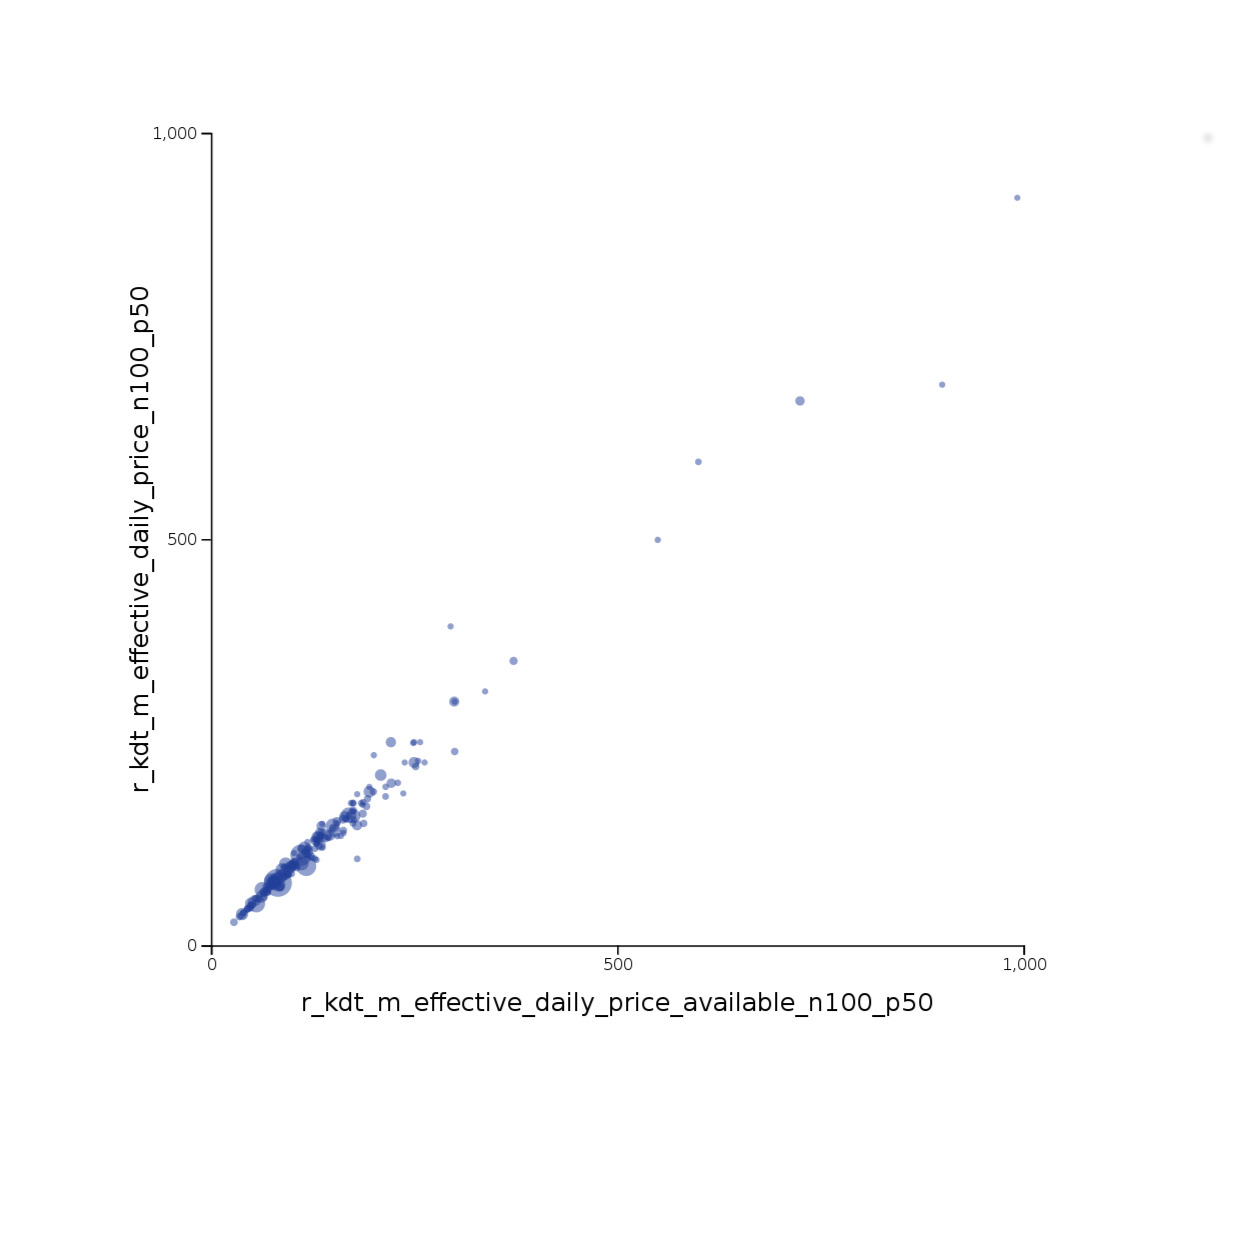
\includegraphics{airbnb_1.png} &
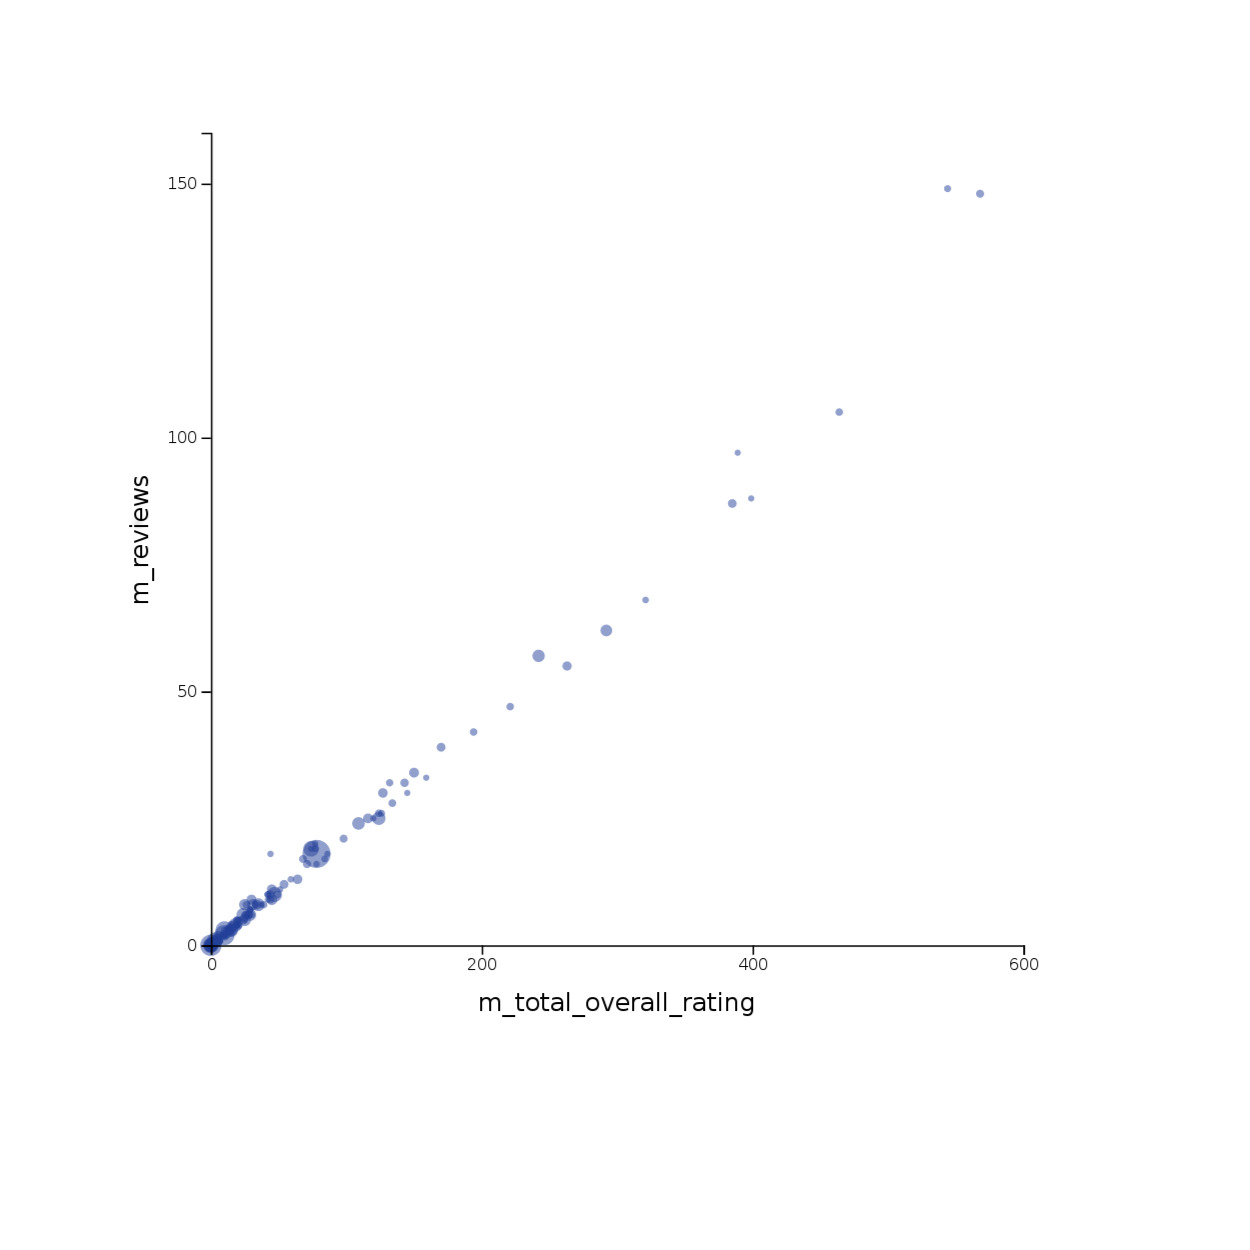
\includegraphics{airbnb_2.png}\tabularnewline
\bottomrule
\end{longtable}

\begin{longtable}[]{@{}lll@{}}
\toprule
A & B & C\tabularnewline
\midrule
\endhead
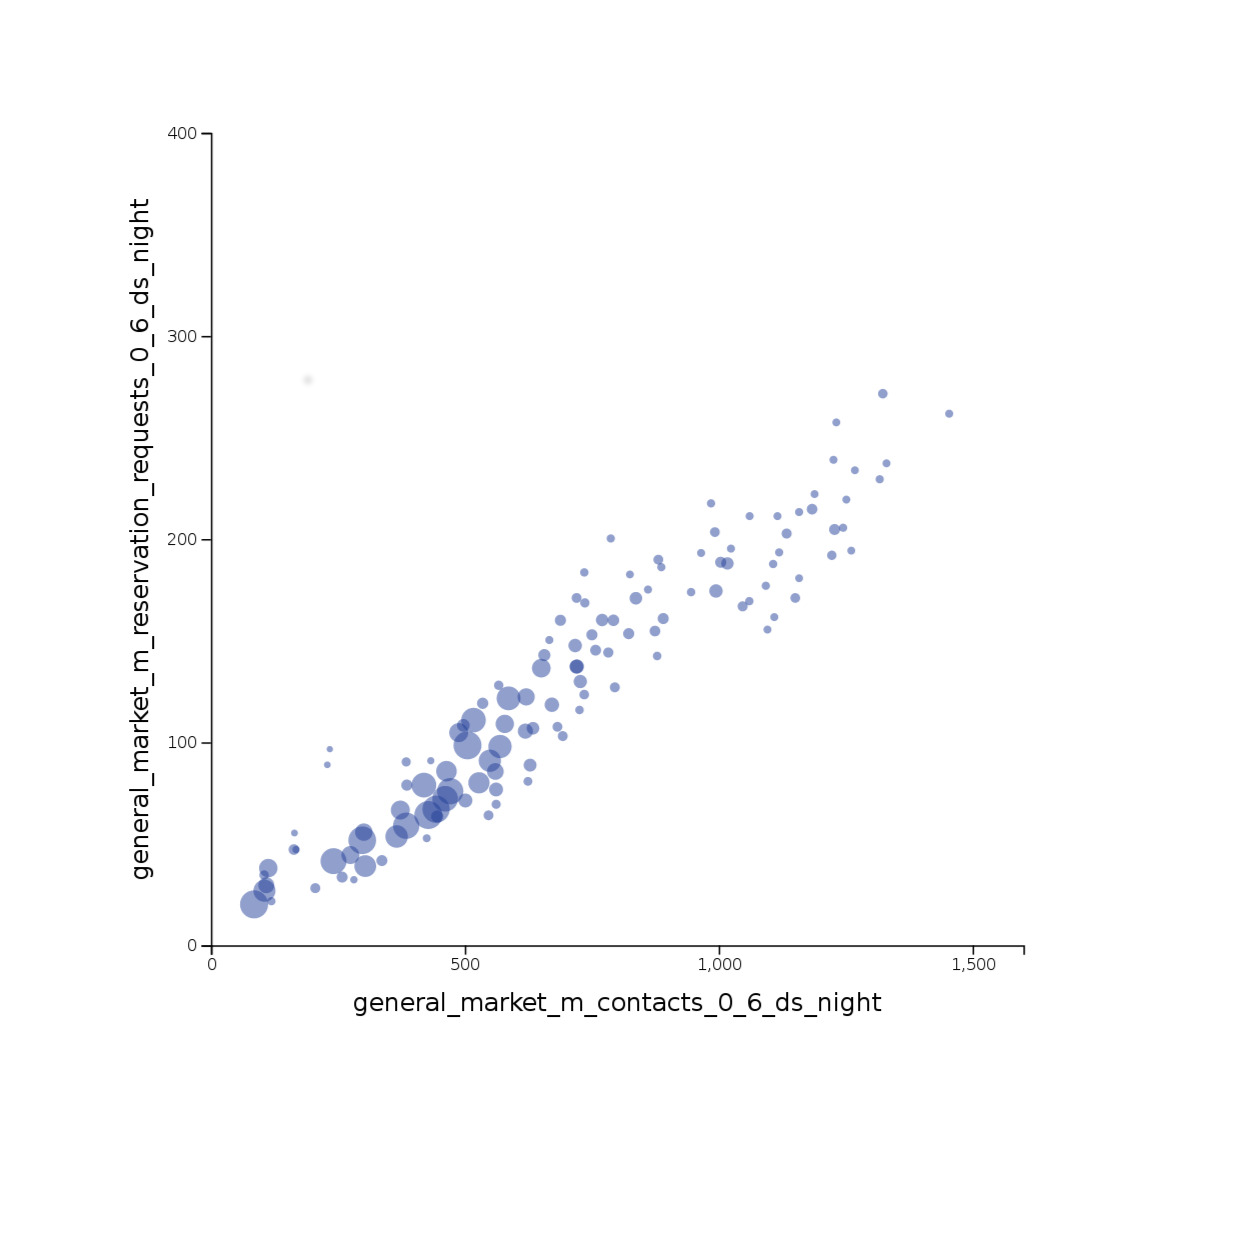
\includegraphics{file-5.png} & 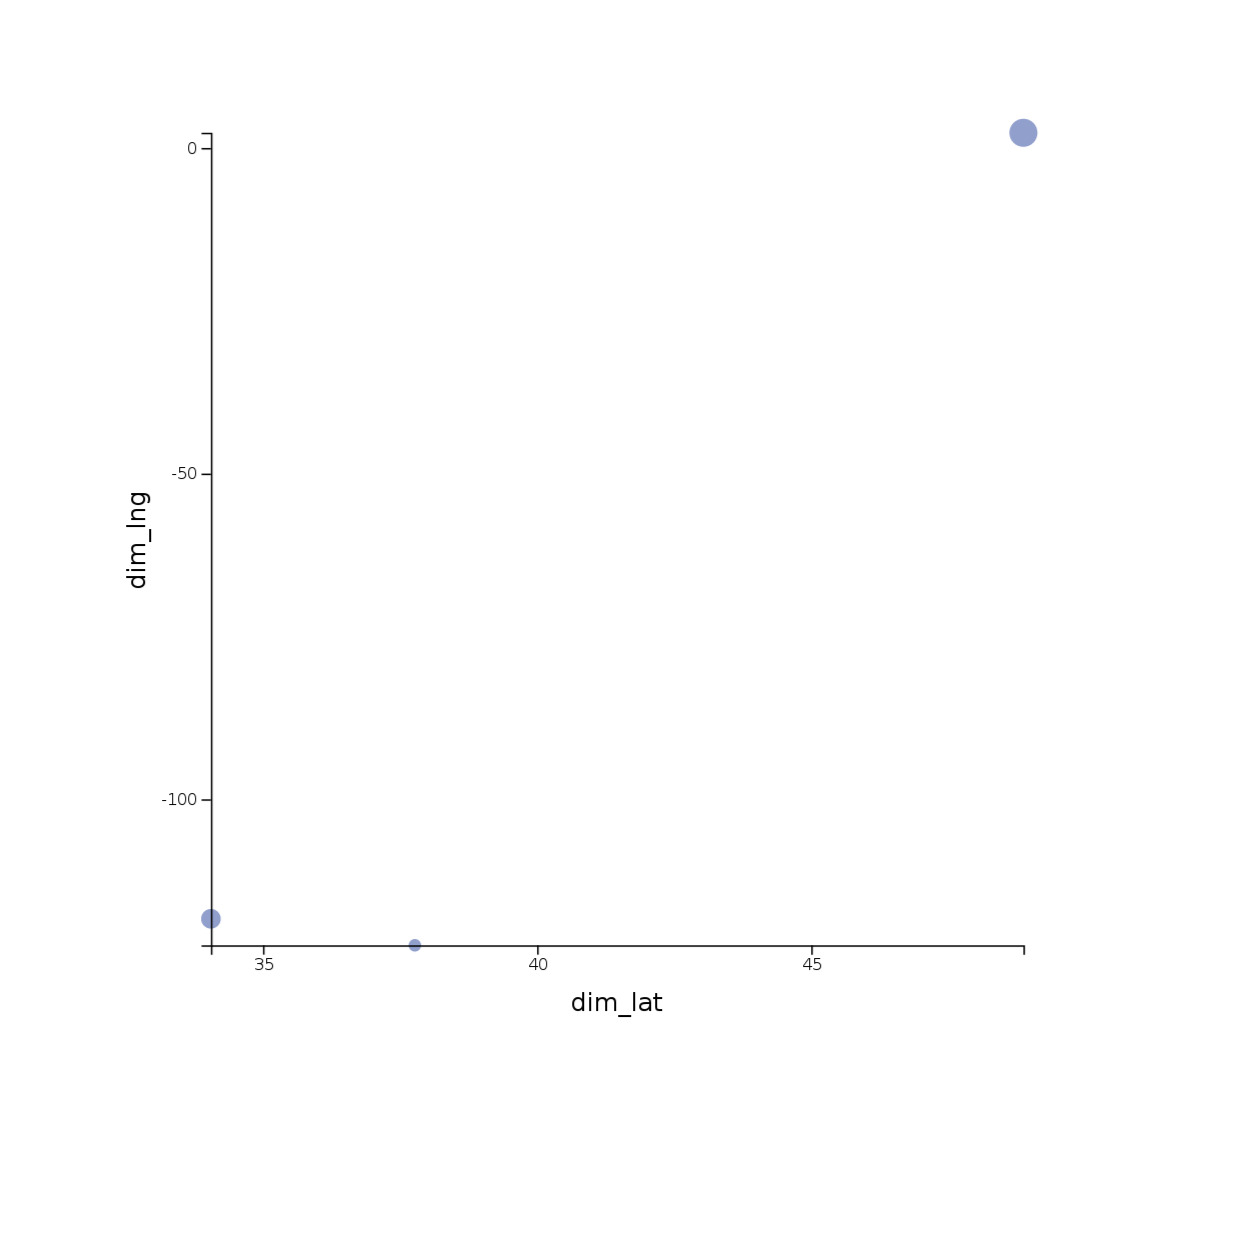
\includegraphics{file-6.png} &
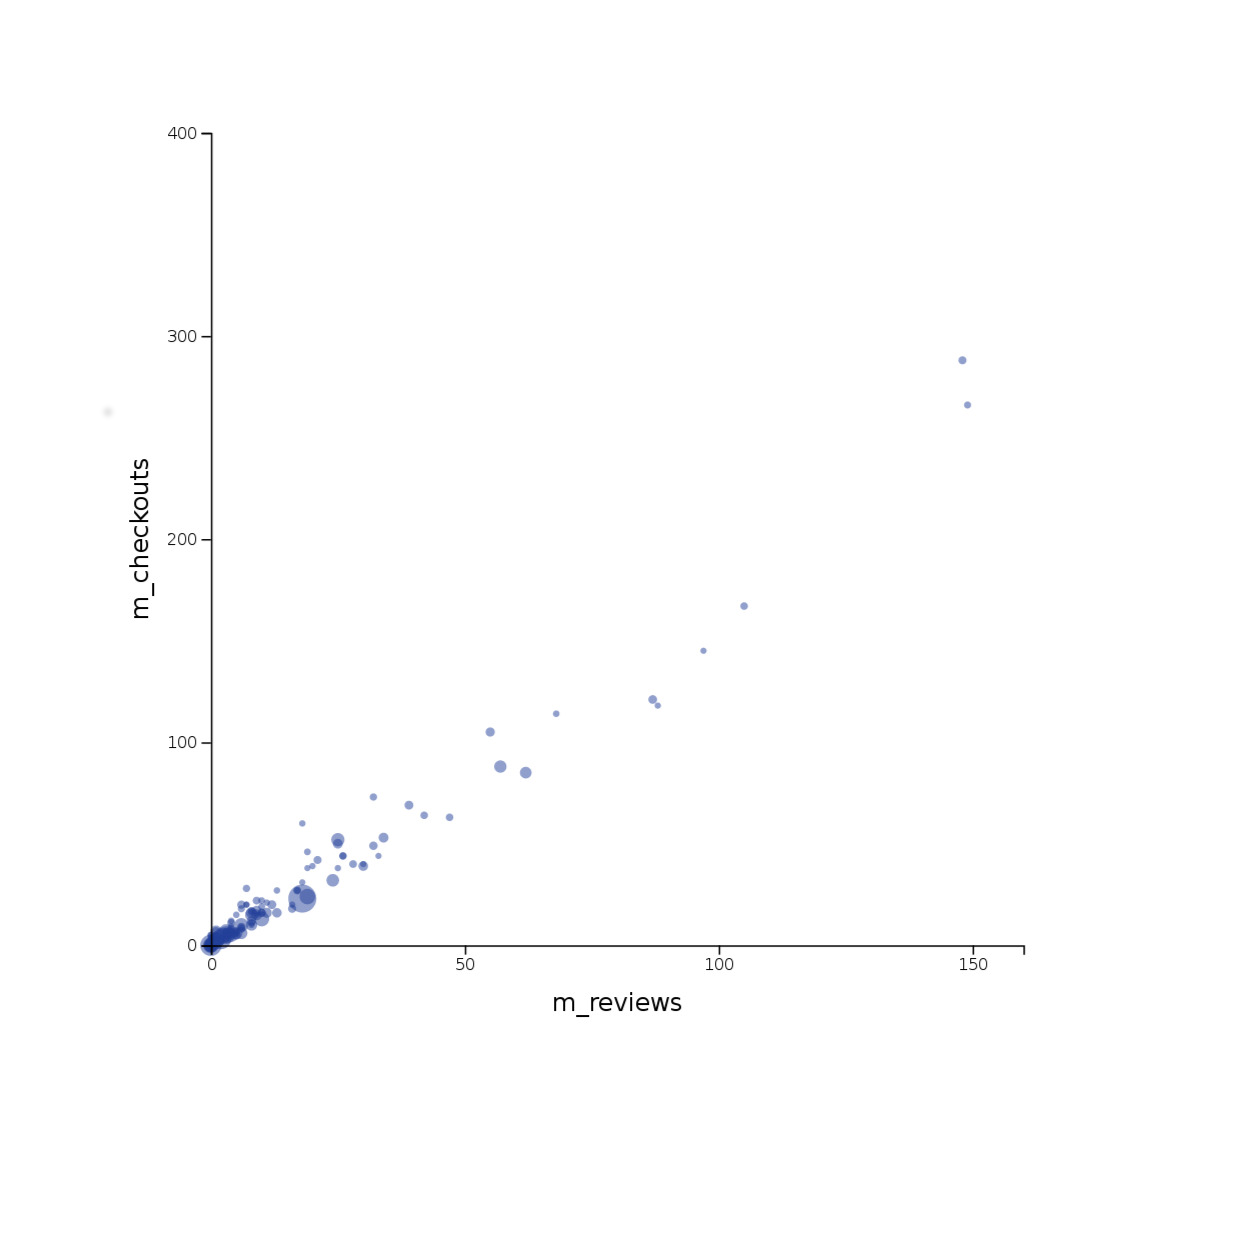
\includegraphics{file-8.png}\tabularnewline
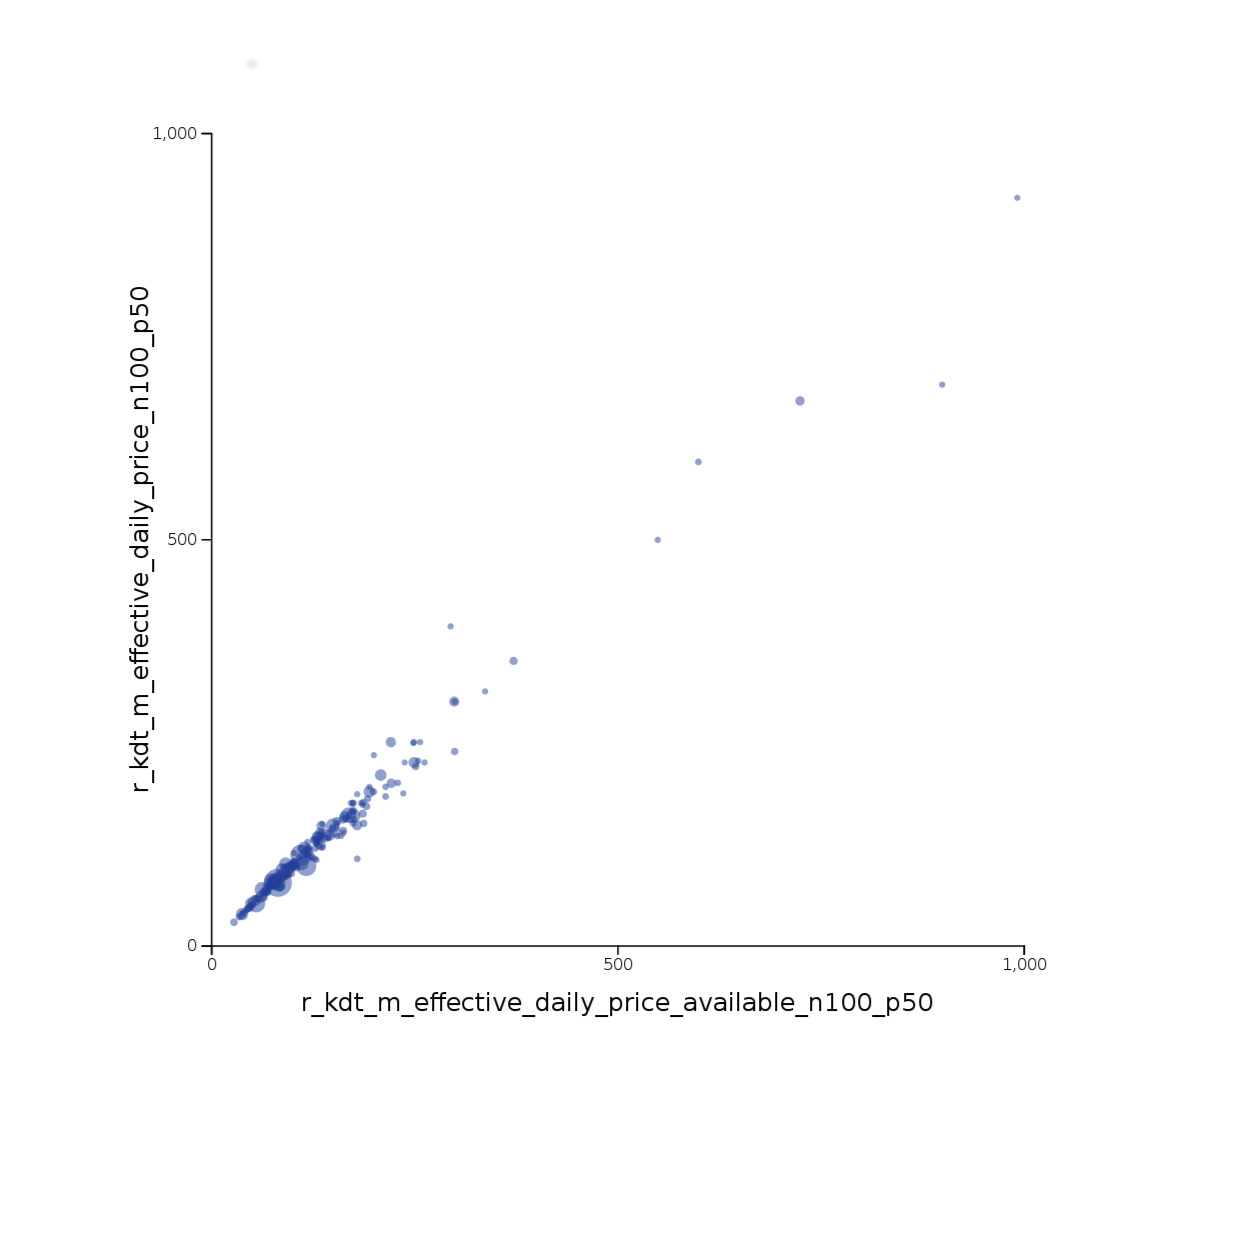
\includegraphics{file-9.png} & 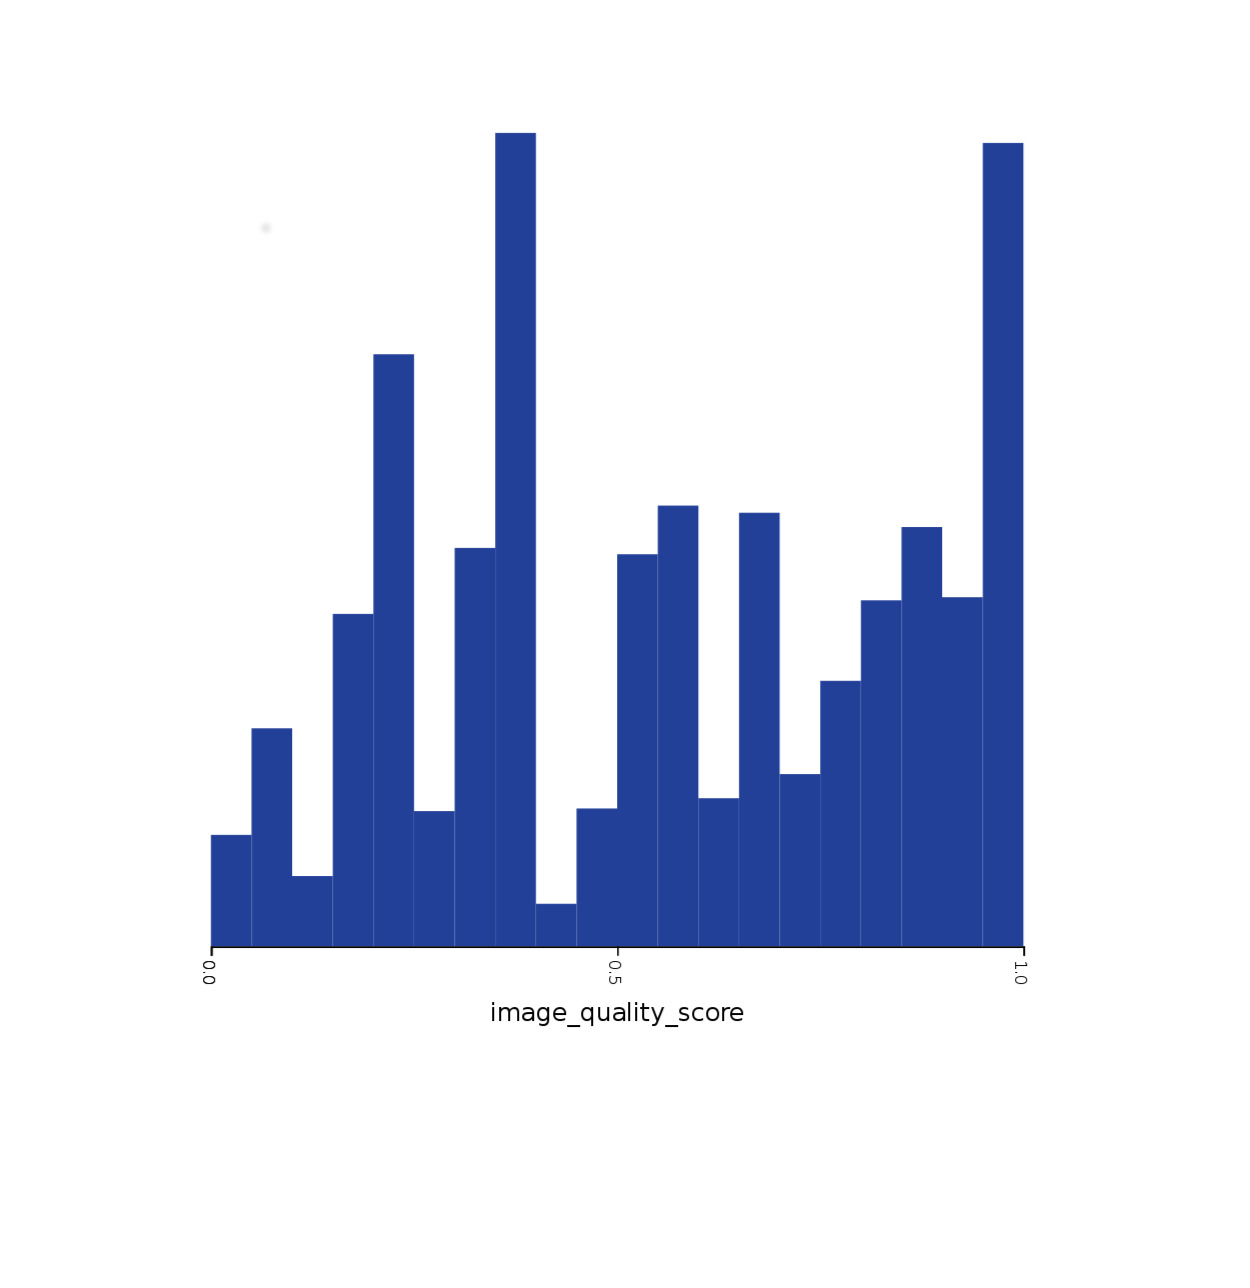
\includegraphics{image_quality_score.png}
&
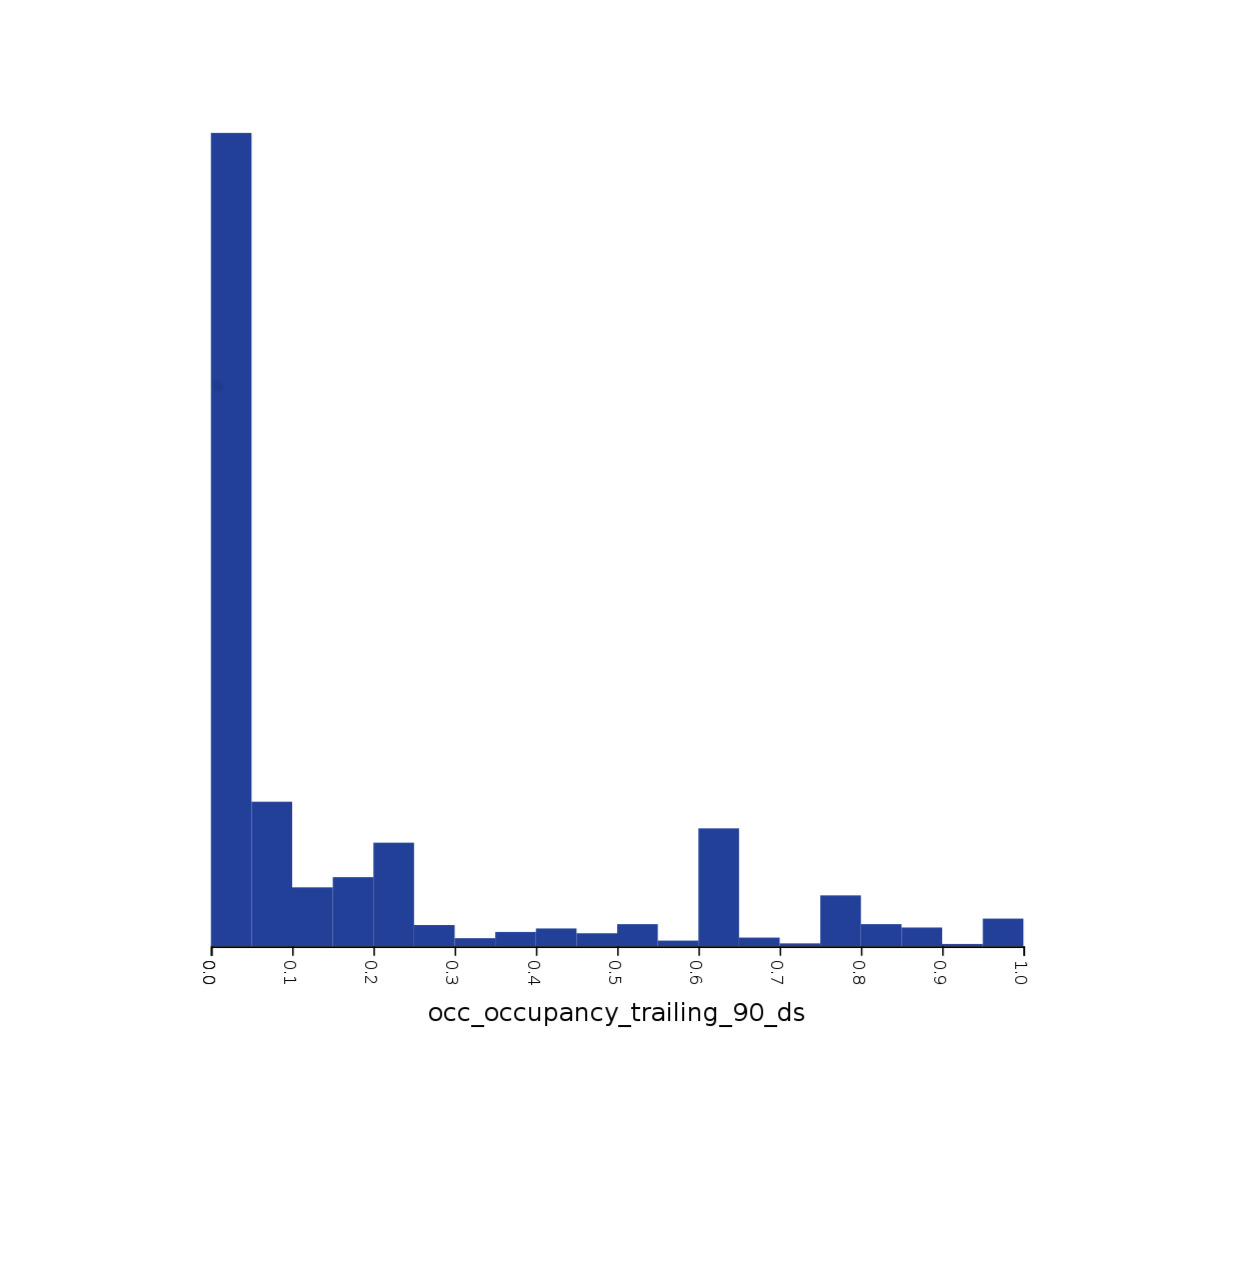
\includegraphics{occ_occupancy_trailing_90_ds_zerobin.png}\tabularnewline
\includegraphics{price_booked_most_recent_under500vsover500model.png} &
\includegraphics{boxplot_dim_room_type.png} &
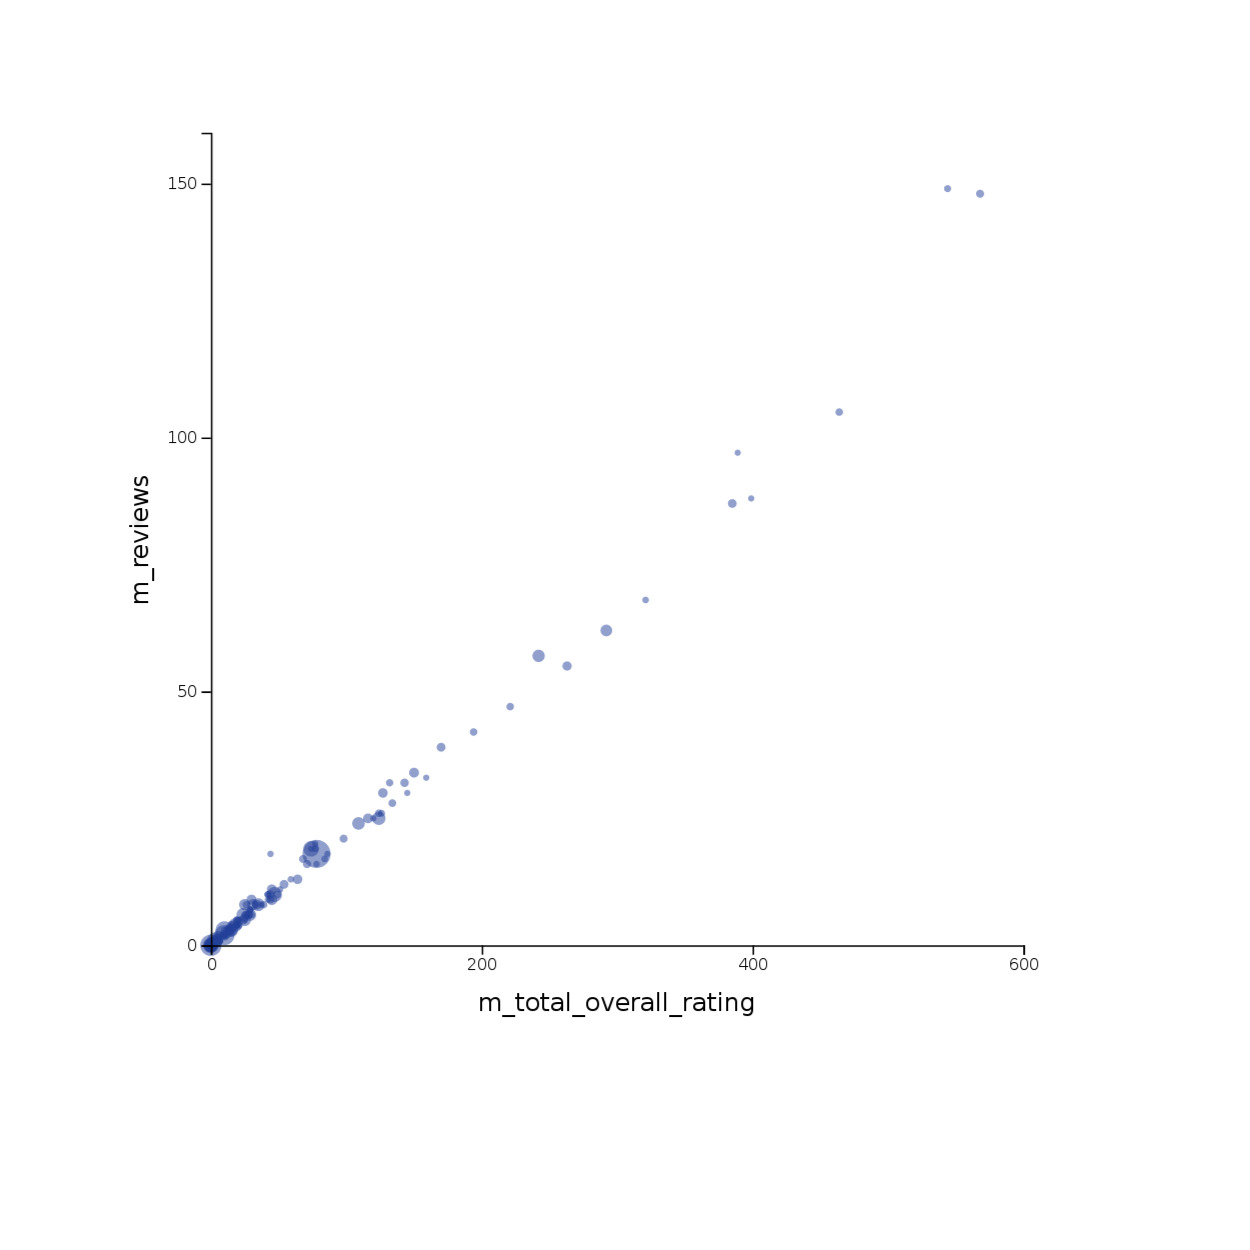
\includegraphics{airbnb_2.png}\tabularnewline
\bottomrule
\end{longtable}

    \paragraph{What other prediction problems can be solved using this
dataset? Suggest future work that could leverage this
data.}\label{what-other-prediction-problems-can-be-solved-using-this-dataset-suggest-future-work-that-could-leverage-this-data.}

Few predictions challenges that can leverage this data:

\begin{itemize}
\item
  What is the best price for my AirBnB: Can you predict the effective
  daily price, value that increases the count of positive dim\_requested
  and make the recommnadation: 1- grouped by market 2- grouped by
  geo-location clusters (locality)
\item
  Where is the hottest market next year? Compare three markets
  seperately: how bookings in one market (e.g. France) affects another
  market. Do they grow together or not? Which neighbor hood will be
  hotest market next?
\end{itemize}

Try the following for detrending:

\begin{itemize}
\tightlist
\item
  Find months with the highest false dim\_requested ratio (not
  requested) try to remove the impacts of this variable as much as
  possible (XGBoost extrapolates very strongly and overfits)
\end{itemize}

\subparagraph{Follwing features together can be very helpful for these
new
challenges/work:}\label{follwing-features-together-can-be-very-helpful-for-these-new-challengeswork}

grouped together: alisting\_anon\_ with m\_checkouts\_price\_ and
booked\_most\_recent

grouped together: Frequency values of listing\_m and
listing\_views\_2\_6\_ds\_night\_decay

grouped together: {[}'ids\_night\_day\_of\_year',
'm\_effective\_daily\_price'{]} columns \#0 (n

\subparagraph{Log transform of the following will be
helpful:}\label{log-transform-of-the-following-will-be-helpful}

m\_effective\_daily\_price count of mapping of id\_listing\_anon
m\_checkouts kdt\_score

    \paragraph{Identify how you would use your model and findings to improve
Airbnb's marketplace by writing out specific
recommendations.}\label{identify-how-you-would-use-your-model-and-findings-to-improve-airbnbs-marketplace-by-writing-out-specific-recommendations.}

based on the model predicts contact Hosts through email and build
engaging value-based marketing efforts: "what are the best things to
know?", Ask for feedback. Ask how involved they are with process
(survey) and if they would recommend the service. Ship marketing camps
to the hosts of higher likelihood of dim\_request. Engage the low
quartile as well (what they need to improve (could be a price update/use
of professional pics, et.c)

    \subsubsection{Step 1. Import and Clean
Data}\label{step-1.-import-and-clean-data}

Start by importing the raw AirBnB data, tab deliminated format.

    \begin{Verbatim}[commandchars=\\\{\}]
{\color{incolor}In [{\color{incolor}1}]:} \PY{k+kn}{import} \PY{n+nn}{numpy} \PY{k}{as} \PY{n+nn}{np}
        \PY{k+kn}{import} \PY{n+nn}{pandas} \PY{k}{as} \PY{n+nn}{pd} 
        \PY{k+kn}{import} \PY{n+nn}{matplotlib}\PY{n+nn}{.}\PY{n+nn}{pyplot} \PY{k}{as} \PY{n+nn}{plt}
        
        \PY{k+kn}{from} \PY{n+nn}{sklearn}\PY{n+nn}{.}\PY{n+nn}{model\PYZus{}selection} \PY{k}{import} \PY{n}{train\PYZus{}test\PYZus{}split}
        
        \PY{k+kn}{from} \PY{n+nn}{sklearn}\PY{n+nn}{.}\PY{n+nn}{pipeline} \PY{k}{import} \PY{n}{Pipeline}
        \PY{k+kn}{from} \PY{n+nn}{sklearn}\PY{n+nn}{.}\PY{n+nn}{preprocessing} \PY{k}{import} \PY{n}{StandardScaler}
        \PY{k+kn}{from} \PY{n+nn}{sklearn}\PY{n+nn}{.}\PY{n+nn}{ensemble} \PY{k}{import} \PY{n}{RandomForestClassifier}
        \PY{k+kn}{from} \PY{n+nn}{sklearn}\PY{n+nn}{.}\PY{n+nn}{linear\PYZus{}model} \PY{k}{import} \PY{n}{SGDClassifier}
        \PY{k+kn}{from} \PY{n+nn}{sklearn}\PY{n+nn}{.}\PY{n+nn}{model\PYZus{}selection} \PY{k}{import} \PY{n}{GridSearchCV}
        \PY{k+kn}{from} \PY{n+nn}{sklearn}\PY{n+nn}{.}\PY{n+nn}{metrics} \PY{k}{import} \PY{n}{matthews\PYZus{}corrcoef}
        
        \PY{k+kn}{from} \PY{n+nn}{sklearn}\PY{n+nn}{.}\PY{n+nn}{metrics} \PY{k}{import} \PY{n}{confusion\PYZus{}matrix}\PY{p}{,} \PY{n}{make\PYZus{}scorer}\PY{p}{,} \PY{n}{classification\PYZus{}report}\PY{p}{,} \PY{n}{cohen\PYZus{}kappa\PYZus{}score}\PY{p}{,} \PY{n}{accuracy\PYZus{}score}\PY{p}{,} \PY{n}{average\PYZus{}precision\PYZus{}score}\PY{p}{,} \PY{n}{roc\PYZus{}auc\PYZus{}score}
        
        
        \PY{k+kn}{import} \PY{n+nn}{warnings}
        
        \PY{k+kn}{import} \PY{n+nn}{itertools}
\end{Verbatim}


    \begin{Verbatim}[commandchars=\\\{\}]
{\color{incolor}In [{\color{incolor}4}]:} \PY{k+kn}{import} \PY{n+nn}{h2o}
        \PY{k+kn}{from} \PY{n+nn}{h2o}\PY{n+nn}{.}\PY{n+nn}{estimators} \PY{k}{import} \PY{n}{H2OGradientBoostingEstimator}
        
        
        \PY{k+kn}{from} \PY{n+nn}{h2o}\PY{n+nn}{.}\PY{n+nn}{estimators}\PY{n+nn}{.}\PY{n+nn}{random\PYZus{}forest} \PY{k}{import} \PY{n}{H2ORandomForestEstimator}
        \PY{k+kn}{from} \PY{n+nn}{h2o}\PY{n+nn}{.}\PY{n+nn}{estimators}\PY{n+nn}{.}\PY{n+nn}{gbm} \PY{k}{import} \PY{n}{H2OGradientBoostingEstimator}
        \PY{k+kn}{from} \PY{n+nn}{h2o}\PY{n+nn}{.}\PY{n+nn}{estimators}\PY{n+nn}{.}\PY{n+nn}{stackedensemble} \PY{k}{import} \PY{n}{H2OStackedEnsembleEstimator}
        \PY{k+kn}{from} \PY{n+nn}{h2o}\PY{n+nn}{.}\PY{n+nn}{grid}\PY{n+nn}{.}\PY{n+nn}{grid\PYZus{}search} \PY{k}{import} \PY{n}{H2OGridSearch}
        \PY{c+c1}{\PYZsh{}from \PYZus{}\PYZus{}future\PYZus{}\PYZus{} import print\PYZus{}function}
        
        \PY{n}{h2o}\PY{o}{.}\PY{n}{init}\PY{p}{(}\PY{n}{ip}\PY{o}{=}\PY{l+s+s2}{\PYZdq{}}\PY{l+s+s2}{127.0.0.1}\PY{l+s+s2}{\PYZdq{}} \PY{p}{,} \PY{n}{port} \PY{o}{=} \PY{l+m+mi}{5151}\PY{p}{,} \PY{n}{max\PYZus{}mem\PYZus{}size}\PY{o}{=}\PY{l+s+s2}{\PYZdq{}}\PY{l+s+s2}{14g}\PY{l+s+s2}{\PYZdq{}}\PY{p}{)}
\end{Verbatim}


    \begin{Verbatim}[commandchars=\\\{\}]
Checking whether there is an H2O instance running at http://127.0.0.1:5151{\ldots} not found.
Attempting to start a local H2O server{\ldots}
  Java Version: openjdk version "1.8.0\_191"; OpenJDK Runtime Environment (build 1.8.0\_191-b12); OpenJDK 64-Bit Server VM (build 25.191-b12, mixed mode)
  Starting server from /home/scv/.local/lib/python3.7/site-packages/h2o/backend/bin/h2o.jar
  Ice root: /tmp/tmpp0k9cd1l
  JVM stdout: /tmp/tmpp0k9cd1l/h2o\_CORP\_scv\_started\_from\_python.out
  JVM stderr: /tmp/tmpp0k9cd1l/h2o\_CORP\_scv\_started\_from\_python.err
  Server is running at http://127.0.0.1:5151
Connecting to H2O server at http://127.0.0.1:5151{\ldots} successful.

    \end{Verbatim}

    
    \begin{verbatim}
--------------------------  ----------------------------------------
H2O cluster uptime:         01 secs
H2O cluster timezone:       America/New_York
H2O data parsing timezone:  UTC
H2O cluster version:        3.22.1.3
H2O cluster version age:    14 days, 14 hours and 47 minutes
H2O cluster name:           H2O_from_python_CORP_scv_bma6od
H2O cluster total nodes:    1
H2O cluster free memory:    12.44 Gb
H2O cluster total cores:    4
H2O cluster allowed cores:  4
H2O cluster status:         accepting new members, healthy
H2O connection url:         http://127.0.0.1:5151
H2O connection proxy:
H2O internal security:      False
H2O API Extensions:         XGBoost, Algos, AutoML, Core V3, Core V4
Python version:             3.7.1 final
--------------------------  ----------------------------------------
    \end{verbatim}

    
    \begin{Verbatim}[commandchars=\\\{\}]
{\color{incolor}In [{\color{incolor}5}]:} \PY{n}{data\PYZus{}path} \PY{o}{=} \PY{l+s+s2}{\PYZdq{}}\PY{l+s+s2}{https://s3.amazonaws.com/challengeprivate/TH\PYZus{}data\PYZus{}challenge.tsv}\PY{l+s+s2}{\PYZdq{}}
        \PY{c+c1}{\PYZsh{}data = pd.read\PYZus{}csv(data\PYZus{}path ,delimiter=\PYZsq{}\PYZbs{}t\PYZsq{},encoding=\PYZsq{}utf\PYZhy{}8\PYZsq{})}
        \PY{n}{data} \PY{o}{=} \PY{n}{h2o}\PY{o}{.}\PY{n}{import\PYZus{}file}\PY{p}{(}\PY{n}{data\PYZus{}path}\PY{p}{,} \PY{n}{destination\PYZus{}frame} \PY{o}{=} \PY{l+s+s2}{\PYZdq{}}\PY{l+s+s2}{airbnb\PYZus{}challenge\PYZus{}raw}\PY{l+s+s2}{\PYZdq{}}\PY{p}{)}
\end{Verbatim}


    \begin{Verbatim}[commandchars=\\\{\}]
Parse progress: |█████████████████████████████████████████████████████████| 100\%

    \end{Verbatim}

    \begin{Verbatim}[commandchars=\\\{\}]
{\color{incolor}In [{\color{incolor}6}]:} \PY{n}{data}\PY{o}{.}\PY{n}{head}\PY{p}{(}\PY{p}{)}
\end{Verbatim}


    
    
\begin{Verbatim}[commandchars=\\\{\}]
{\color{outcolor}Out[{\color{outcolor}6}]:} 
\end{Verbatim}
            
    Starting strong: For building up from the base model onwards we want to
see how balanced is predicting variable. We will use most of the numeric
features and few categorical. Let's talk a look and make sure we are
touching anything that requires processing (NaN, high cardinality,
etc.).

    \begin{Verbatim}[commandchars=\\\{\}]
{\color{incolor}In [{\color{incolor}7}]:} \PY{n}{data}\PY{p}{[}\PY{l+s+s2}{\PYZdq{}}\PY{l+s+s2}{dim\PYZus{}is\PYZus{}requested}\PY{l+s+s2}{\PYZdq{}}\PY{p}{]}\PY{o}{.}\PY{n}{table}\PY{p}{(}\PY{p}{)}
\end{Verbatim}


    
    
\begin{Verbatim}[commandchars=\\\{\}]
{\color{outcolor}Out[{\color{outcolor}7}]:} 
\end{Verbatim}
            
    \begin{Verbatim}[commandchars=\\\{\}]
{\color{incolor}In [{\color{incolor}8}]:} \PY{n}{data}\PY{p}{[}\PY{l+s+s2}{\PYZdq{}}\PY{l+s+s2}{ds\PYZus{}checkin\PYZus{}gap}\PY{l+s+s2}{\PYZdq{}}\PY{p}{]}\PY{o}{.}\PY{n}{table}\PY{p}{(}\PY{p}{)}
\end{Verbatim}


    
    
\begin{Verbatim}[commandchars=\\\{\}]
{\color{outcolor}Out[{\color{outcolor}8}]:} 
\end{Verbatim}
            
    XXThe columns and emp\_length are being treated as categoricals instead
of numeric because the unit of measure is included. Machine learning
algorithms will treat this as a categorical and will not understand that
8 years is closer to 9 years than 1 year. To recitify this, we will use
H2O to remove the units of measure and convert the column to numeric.

    Our last cleaning step will be to remove all columns that are not
relevant to our use case. Some columns we will not use because they have
data leakage.

    The splits is done on the all data 0.70, 0.15, 0.15- training,
validation and test set so that the distribution in the training,
validation and test set are the same as much as possible and the
imblance is not affecting the modeling.

    \begin{Verbatim}[commandchars=\\\{\}]
{\color{incolor}In [{\color{incolor}34}]:} \PY{c+c1}{\PYZsh{}df\PYZus{}train, df\PYZus{}valid, df\PYZus{}test = data.split\PYZus{}frame(ratios=[.7, .15], seed = 1234) \PYZsh{}training .70 validation .15 and final scoring on testing .15}
         \PY{k}{def} \PY{n+nf}{au\PYZus{}data\PYZus{}split}\PY{p}{(}\PY{n}{dataobj} \PY{o}{=} \PY{n}{data}\PY{p}{,} \PY{n}{trainsp} \PY{o}{=} \PY{l+m+mf}{0.7}\PY{p}{,} \PY{n}{val\PYZus{}testsp}\PY{o}{=}\PY{l+m+mf}{0.15}\PY{p}{)}\PY{p}{:}
             \PY{n}{n\PYZus{}size} \PY{o}{=}\PY{l+m+mi}{184279}
             \PY{n}{sploc1} \PY{o}{=} \PY{n+nb}{round}\PY{p}{(}\PY{n}{trainsp}\PY{o}{*}\PY{n}{n\PYZus{}size}\PY{p}{)}
             \PY{n}{sploc2} \PY{o}{=} \PY{n}{sploc1} \PY{o}{+} \PY{n+nb}{round}\PY{p}{(}\PY{n}{val\PYZus{}testsp}\PY{o}{*}\PY{n}{n\PYZus{}size}\PY{p}{)}
             
             \PY{n}{df\PYZus{}train} \PY{o}{=} \PY{n}{data}\PY{p}{[}\PY{n+nb}{range}\PY{p}{(}\PY{l+m+mi}{0}\PY{p}{,}\PY{n}{sploc1}\PY{p}{)}\PY{p}{,}\PY{p}{:}\PY{p}{]}
             \PY{n}{df\PYZus{}valid} \PY{o}{=} \PY{n}{data}\PY{p}{[}\PY{n+nb}{range}\PY{p}{(}\PY{n}{sploc1}\PY{o}{+}\PY{l+m+mi}{1}\PY{p}{,}\PY{n}{sploc2}\PY{p}{)}\PY{p}{,}\PY{p}{:}\PY{p}{]}
             \PY{n}{df\PYZus{}test}  \PY{o}{=} \PY{n}{data}\PY{p}{[}\PY{n+nb}{range}\PY{p}{(}\PY{n}{sploc2}\PY{o}{+}\PY{l+m+mi}{1}\PY{p}{,}\PY{n}{n\PYZus{}size}\PY{p}{)}\PY{p}{,}\PY{p}{:}\PY{p}{]}
             \PY{c+c1}{\PYZsh{}print(\PYZdq{}training split\PYZdq{}, df\PYZus{}train.describe)}
             \PY{c+c1}{\PYZsh{}print(\PYZdq{}validation split\PYZdq{}, df\PYZus{}valid.describe)}
             \PY{c+c1}{\PYZsh{}print(\PYZdq{}testing split\PYZdq{}, df\PYZus{}test.describe)}
             \PY{k}{return}\PY{p}{(}\PY{n}{df\PYZus{}train}\PY{p}{,} \PY{n}{df\PYZus{}valid}\PY{p}{,} \PY{n}{df\PYZus{}test}\PY{p}{)}
             
         
         \PY{n}{df\PYZus{}train}\PY{p}{,} \PY{n}{df\PYZus{}valid}\PY{p}{,} \PY{n}{df\PYZus{}test} \PY{o}{=} \PY{n}{au\PYZus{}data\PYZus{}split}\PY{p}{(}\PY{n}{data}\PY{p}{,} \PY{l+m+mf}{0.7}\PY{p}{,} \PY{l+m+mf}{0.15}\PY{p}{)}
         
         \PY{n}{h2o}\PY{o}{.}\PY{n}{export\PYZus{}file}\PY{p}{(} \PY{n}{df\PYZus{}train}\PY{p}{,} \PY{n}{path}\PY{o}{=} \PY{l+s+s1}{\PYZsq{}}\PY{l+s+s1}{data\PYZus{}train\PYZus{}c0.csv}\PY{l+s+s1}{\PYZsq{}}\PY{p}{)}
         \PY{n}{h2o}\PY{o}{.}\PY{n}{export\PYZus{}file}\PY{p}{(} \PY{n}{df\PYZus{}valid}\PY{p}{,} \PY{n}{path}\PY{o}{=} \PY{l+s+s1}{\PYZsq{}}\PY{l+s+s1}{data\PYZus{}valid\PYZus{}c0.csv}\PY{l+s+s1}{\PYZsq{}}\PY{p}{)}
         \PY{n}{h2o}\PY{o}{.}\PY{n}{export\PYZus{}file}\PY{p}{(} \PY{n}{df\PYZus{}test}\PY{p}{,} \PY{n}{path}\PY{o}{=} \PY{l+s+s1}{\PYZsq{}}\PY{l+s+s1}{data\PYZus{}test\PYZus{}c0.csv}\PY{l+s+s1}{\PYZsq{}}\PY{p}{)}
\end{Verbatim}


    \begin{Verbatim}[commandchars=\\\{\}]
Export File progress: |███████████████████████████████████████████████████| 100\%
Export File progress: |███████████████████████████████████████████████████| 100\%
Export File progress: |███████████████████████████████████████████████████| 100\%

    \end{Verbatim}

    \subsection{Step 2. Train Baseline
Model}\label{step-2.-train-baseline-model}

We will train an initial model. The goal of our initial model is to
provide a baseline AUC that we will try to beat with our feature
engineering.

    \begin{Verbatim}[commandchars=\\\{\}]
{\color{incolor}In [{\color{incolor}10}]:} \PY{c+c1}{\PYZsh{} Filter to relevant columns}
         \PY{n}{relevant\PYZus{}cols} \PY{o}{=} \PY{p}{[} 
         \PY{l+s+s1}{\PYZsq{}}\PY{l+s+s1}{dim\PYZus{}is\PYZus{}requested}\PY{l+s+s1}{\PYZsq{}}\PY{p}{,}
         \PY{l+s+s1}{\PYZsq{}}\PY{l+s+s1}{ds\PYZus{}night}\PY{l+s+s1}{\PYZsq{}}\PY{p}{,} 
         \PY{l+s+s1}{\PYZsq{}}\PY{l+s+s1}{id\PYZus{}listing\PYZus{}anon}\PY{l+s+s1}{\PYZsq{}}\PY{p}{,} 
         \PY{l+s+s1}{\PYZsq{}}\PY{l+s+s1}{m\PYZus{}effective\PYZus{}daily\PYZus{}price}\PY{l+s+s1}{\PYZsq{}}\PY{p}{,}
         \PY{l+s+s1}{\PYZsq{}}\PY{l+s+s1}{m\PYZus{}pricing\PYZus{}cleaning\PYZus{}fee}\PY{l+s+s1}{\PYZsq{}}\PY{p}{,} 
         \PY{c+c1}{\PYZsh{}needs cleaning  \PYZsq{}dim\PYZus{}market\PYZsq{}, }
         \PY{c+c1}{\PYZsh{}use kdt instead \PYZsq{}dim\PYZus{}lat\PYZsq{}, }
         \PY{c+c1}{\PYZsh{}use kdt instead \PYZsq{}dim\PYZus{}lng\PYZsq{}, }
         \PY{c+c1}{\PYZsh{}needs process  \PYZsq{}dim\PYZus{}room\PYZus{}type\PYZsq{},}
         \PY{l+s+s1}{\PYZsq{}}\PY{l+s+s1}{dim\PYZus{}person\PYZus{}capacity}\PY{l+s+s1}{\PYZsq{}}\PY{p}{,} \PY{c+c1}{\PYZsh{}num}
         \PY{l+s+s1}{\PYZsq{}}\PY{l+s+s1}{dim\PYZus{}is\PYZus{}instant\PYZus{}bookable}\PY{l+s+s1}{\PYZsq{}}\PY{p}{,} \PY{c+c1}{\PYZsh{}bool}
         \PY{l+s+s1}{\PYZsq{}}\PY{l+s+s1}{m\PYZus{}checkouts}\PY{l+s+s1}{\PYZsq{}}\PY{p}{,}  \PY{c+c1}{\PYZsh{}num}
         \PY{l+s+s1}{\PYZsq{}}\PY{l+s+s1}{m\PYZus{}reviews}\PY{l+s+s1}{\PYZsq{}}\PY{p}{,} \PY{c+c1}{\PYZsh{}num}
         \PY{l+s+s1}{\PYZsq{}}\PY{l+s+s1}{days\PYZus{}since\PYZus{}last\PYZus{}booking}\PY{l+s+s1}{\PYZsq{}}\PY{p}{,} \PY{c+c1}{\PYZsh{}num}
         \PY{l+s+s1}{\PYZsq{}}\PY{l+s+s1}{cancel\PYZus{}policy}\PY{l+s+s1}{\PYZsq{}}\PY{p}{,} \PY{c+c1}{\PYZsh{}cat 3\PYZhy{}9}
         \PY{l+s+s1}{\PYZsq{}}\PY{l+s+s1}{image\PYZus{}quality\PYZus{}score}\PY{l+s+s1}{\PYZsq{}}\PY{p}{,} \PY{c+c1}{\PYZsh{}num}
         \PY{l+s+s1}{\PYZsq{}}\PY{l+s+s1}{m\PYZus{}total\PYZus{}overall\PYZus{}rating}\PY{l+s+s1}{\PYZsq{}}\PY{p}{,} \PY{c+c1}{\PYZsh{}num}
         \PY{l+s+s1}{\PYZsq{}}\PY{l+s+s1}{m\PYZus{}professional\PYZus{}pictures}\PY{l+s+s1}{\PYZsq{}}\PY{p}{,} \PY{c+c1}{\PYZsh{}num}
         \PY{l+s+s1}{\PYZsq{}}\PY{l+s+s1}{dim\PYZus{}has\PYZus{}wireless\PYZus{}internet}\PY{l+s+s1}{\PYZsq{}}\PY{p}{,} \PY{c+c1}{\PYZsh{}bool}
         \PY{l+s+s1}{\PYZsq{}}\PY{l+s+s1}{ds\PYZus{}night\PYZus{}day\PYZus{}of\PYZus{}week}\PY{l+s+s1}{\PYZsq{}}\PY{p}{,} \PY{c+c1}{\PYZsh{}bool}
         \PY{l+s+s1}{\PYZsq{}}\PY{l+s+s1}{ds\PYZus{}night\PYZus{}day\PYZus{}of\PYZus{}year}\PY{l+s+s1}{\PYZsq{}}\PY{p}{,} \PY{c+c1}{\PYZsh{}bool}
         \PY{l+s+s1}{\PYZsq{}}\PY{l+s+s1}{ds\PYZus{}checkin\PYZus{}gap}\PY{l+s+s1}{\PYZsq{}}\PY{p}{,} \PY{c+c1}{\PYZsh{}num 0\PYZhy{}6}
         \PY{l+s+s1}{\PYZsq{}}\PY{l+s+s1}{ds\PYZus{}checkout\PYZus{}gap}\PY{l+s+s1}{\PYZsq{}}\PY{p}{,} \PY{c+c1}{\PYZsh{}num 0\PYZhy{}6}
         \PY{l+s+s1}{\PYZsq{}}\PY{l+s+s1}{occ\PYZus{}occupancy\PYZus{}plus\PYZus{}minus\PYZus{}7\PYZus{}ds\PYZus{}night}\PY{l+s+s1}{\PYZsq{}}\PY{p}{,} \PY{c+c1}{\PYZsh{}num }
         \PY{l+s+s1}{\PYZsq{}}\PY{l+s+s1}{occ\PYZus{}occupancy\PYZus{}plus\PYZus{}minus\PYZus{}14\PYZus{}ds\PYZus{}night}\PY{l+s+s1}{\PYZsq{}}\PY{p}{,} \PY{c+c1}{\PYZsh{}num }
         \PY{l+s+s1}{\PYZsq{}}\PY{l+s+s1}{occ\PYZus{}occupancy\PYZus{}trailing\PYZus{}90\PYZus{}ds}\PY{l+s+s1}{\PYZsq{}}\PY{p}{,} \PY{c+c1}{\PYZsh{}num }
         \PY{l+s+s1}{\PYZsq{}}\PY{l+s+s1}{m\PYZus{}minimum\PYZus{}nights}\PY{l+s+s1}{\PYZsq{}}\PY{p}{,} \PY{c+c1}{\PYZsh{}num }
         \PY{c+c1}{\PYZsh{}\PYZsq{}m\PYZus{}maximum\PYZus{}nights\PYZsq{}, }
         \PY{l+s+s1}{\PYZsq{}}\PY{l+s+s1}{price\PYZus{}booked\PYZus{}most\PYZus{}recent}\PY{l+s+s1}{\PYZsq{}}\PY{p}{,} \PY{c+c1}{\PYZsh{}num }
         \PY{l+s+s1}{\PYZsq{}}\PY{l+s+s1}{p2\PYZus{}p3\PYZus{}click\PYZus{}through\PYZus{}score}\PY{l+s+s1}{\PYZsq{}}\PY{p}{,} \PY{c+c1}{\PYZsh{}num }
         \PY{l+s+s1}{\PYZsq{}}\PY{l+s+s1}{p3\PYZus{}inquiry\PYZus{}score}\PY{l+s+s1}{\PYZsq{}}\PY{p}{,}  \PY{c+c1}{\PYZsh{}num }
         \PY{l+s+s1}{\PYZsq{}}\PY{l+s+s1}{listing\PYZus{}m\PYZus{}listing\PYZus{}views\PYZus{}2\PYZus{}6\PYZus{}ds\PYZus{}night\PYZus{}decay}\PY{l+s+s1}{\PYZsq{}}\PY{p}{,} \PY{c+c1}{\PYZsh{}num }
         \PY{c+c1}{\PYZsh{}\PYZsq{}general\PYZus{}market\PYZus{}m\PYZus{}unique\PYZus{}searchers\PYZus{}0\PYZus{}6\PYZus{}ds\PYZus{}night\PYZsq{},\PYZsh{}num }
         \PY{c+c1}{\PYZsh{}\PYZsq{}general\PYZus{}market\PYZus{}m\PYZus{}contacts\PYZus{}0\PYZus{}6\PYZus{}ds\PYZus{}night\PYZsq{},\PYZsh{}num }
         \PY{l+s+s1}{\PYZsq{}}\PY{l+s+s1}{general\PYZus{}market\PYZus{}m\PYZus{}reservation\PYZus{}requests\PYZus{}0\PYZus{}6\PYZus{}ds\PYZus{}night}\PY{l+s+s1}{\PYZsq{}}\PY{p}{,}\PY{c+c1}{\PYZsh{}num }
         \PY{l+s+s1}{\PYZsq{}}\PY{l+s+s1}{general\PYZus{}market\PYZus{}m\PYZus{}is\PYZus{}booked\PYZus{}0\PYZus{}6\PYZus{}ds\PYZus{}night}\PY{l+s+s1}{\PYZsq{}}\PY{p}{,}
         \PY{l+s+s1}{\PYZsq{}}\PY{l+s+s1}{m\PYZus{}available\PYZus{}listings\PYZus{}ds\PYZus{}night}\PY{l+s+s1}{\PYZsq{}}\PY{p}{,}
         \PY{l+s+s1}{\PYZsq{}}\PY{l+s+s1}{kdt\PYZus{}score}\PY{l+s+s1}{\PYZsq{}}\PY{p}{,} 
         \PY{l+s+s1}{\PYZsq{}}\PY{l+s+s1}{r\PYZus{}kdt\PYZus{}listing\PYZus{}views\PYZus{}0\PYZus{}6\PYZus{}avg\PYZus{}n100}\PY{l+s+s1}{\PYZsq{}}\PY{p}{,} 
         \PY{l+s+s1}{\PYZsq{}}\PY{l+s+s1}{r\PYZus{}kdt\PYZus{}n\PYZus{}active\PYZus{}n100}\PY{l+s+s1}{\PYZsq{}}\PY{p}{,} 
         \PY{l+s+s1}{\PYZsq{}}\PY{l+s+s1}{r\PYZus{}kdt\PYZus{}n\PYZus{}available\PYZus{}n100}\PY{l+s+s1}{\PYZsq{}}\PY{p}{,} 
         \PY{l+s+s1}{\PYZsq{}}\PY{l+s+s1}{r\PYZus{}kdt\PYZus{}m\PYZus{}effective\PYZus{}daily\PYZus{}price\PYZus{}n100\PYZus{}p50}\PY{l+s+s1}{\PYZsq{}}\PY{p}{,} 
         \PY{l+s+s1}{\PYZsq{}}\PY{l+s+s1}{r\PYZus{}kdt\PYZus{}m\PYZus{}effective\PYZus{}daily\PYZus{}price\PYZus{}available\PYZus{}n100\PYZus{}p50}\PY{l+s+s1}{\PYZsq{}}\PY{p}{,}
         \PY{l+s+s1}{\PYZsq{}}\PY{l+s+s1}{r\PYZus{}kdt\PYZus{}m\PYZus{}effective\PYZus{}daily\PYZus{}price\PYZus{}booked\PYZus{}n100\PYZus{}p50}\PY{l+s+s1}{\PYZsq{}}
         
         \PY{p}{]}
         
         \PY{n}{data} \PY{o}{=} \PY{n}{data}\PY{p}{[}\PY{n}{relevant\PYZus{}cols}\PY{p}{]}
         \PY{n}{data}\PY{o}{.}\PY{n}{head}\PY{p}{(}\PY{p}{)}
\end{Verbatim}


    
    
\begin{Verbatim}[commandchars=\\\{\}]
{\color{outcolor}Out[{\color{outcolor}10}]:} 
\end{Verbatim}
            
    \begin{Verbatim}[commandchars=\\\{\}]
{\color{incolor}In [{\color{incolor}13}]:} \PY{n}{target} \PY{o}{=} \PY{l+s+s2}{\PYZdq{}}\PY{l+s+s2}{dim\PYZus{}is\PYZus{}requested}\PY{l+s+s2}{\PYZdq{}}
         \PY{n}{predictors} \PY{o}{=} \PY{n+nb}{list}\PY{p}{(}\PY{n+nb}{set}\PY{p}{(}\PY{n}{df\PYZus{}train}\PY{o}{.}\PY{n}{col\PYZus{}names}\PY{p}{)} \PY{o}{\PYZhy{}} \PY{n+nb}{set}\PY{p}{(}\PY{p}{[}\PY{n}{target}\PY{p}{]}\PY{p}{)}\PY{p}{)}
\end{Verbatim}


    \begin{Verbatim}[commandchars=\\\{\}]
{\color{incolor}In [{\color{incolor}14}]:} \PY{c+c1}{\PYZsh{} Train initial GBM model}
         \PY{n}{df\PYZus{}train}\PY{p}{[}\PY{l+s+s2}{\PYZdq{}}\PY{l+s+s2}{dim\PYZus{}is\PYZus{}requested}\PY{l+s+s2}{\PYZdq{}}\PY{p}{]}\PY{o}{.}\PY{n}{asfactor}\PY{p}{(}\PY{p}{)}
         
         \PY{n}{gbm\PYZus{}baseline} \PY{o}{=} \PY{n}{H2OGradientBoostingEstimator}\PY{p}{(}\PY{n}{seed} \PY{o}{=} \PY{l+m+mi}{1234}\PY{p}{,} \PY{n}{model\PYZus{}id} \PY{o}{=} \PY{l+s+s2}{\PYZdq{}}\PY{l+s+s2}{gbm\PYZus{}baseline.hex}\PY{l+s+s2}{\PYZdq{}}\PY{p}{,} 
                                                     \PY{n}{ntrees} \PY{o}{=} \PY{l+m+mi}{500}\PY{p}{,} 
                                                     \PY{n}{stopping\PYZus{}rounds} \PY{o}{=} \PY{l+m+mi}{10}\PY{p}{,} \PY{n}{score\PYZus{}tree\PYZus{}interval} \PY{o}{=} \PY{l+m+mi}{5}\PY{p}{,} \PY{c+c1}{\PYZsh{} early stopping}
                                                     \PY{n}{stopping\PYZus{}metric} \PY{o}{=} \PY{l+s+s2}{\PYZdq{}}\PY{l+s+s2}{AUC}\PY{l+s+s2}{\PYZdq{}}\PY{p}{,}
                                                     \PY{n}{nfolds} \PY{o}{=} \PY{l+m+mi}{5} 
                                                    \PY{p}{)}
         \PY{n}{gbm\PYZus{}baseline}\PY{o}{.}\PY{n}{train}\PY{p}{(}\PY{n}{x} \PY{o}{=} \PY{n}{predictors}\PY{p}{,} \PY{n}{y} \PY{o}{=} \PY{n}{target}\PY{p}{,} \PY{n}{training\PYZus{}frame} \PY{o}{=} \PY{n}{df\PYZus{}train}\PY{p}{)}
\end{Verbatim}


    \begin{Verbatim}[commandchars=\\\{\}]
gbm Model Build progress: |███████████████████████████████████████████████| 100\%

    \end{Verbatim}

    \begin{Verbatim}[commandchars=\\\{\}]
{\color{incolor}In [{\color{incolor}77}]:} \PY{n+nb}{print}\PY{p}{(}\PY{l+s+s2}{\PYZdq{}}\PY{l+s+s2}{AUC on CV: }\PY{l+s+s2}{\PYZdq{}} \PY{o}{+} \PY{n+nb}{str}\PY{p}{(}\PY{n+nb}{round}\PY{p}{(}\PY{n}{gbm\PYZus{}baseline}\PY{o}{.}\PY{n}{auc}\PY{p}{(}\PY{n}{xval} \PY{o}{=} \PY{k+kc}{True}\PY{p}{)}\PY{p}{,} \PY{l+m+mi}{3}\PY{p}{)}\PY{p}{)}\PY{p}{)} \PY{c+c1}{\PYZsh{}This was done for a random split, no seed on split, AUC without seed change: +0.008, same size 0.7,0.15,0.15. }
\end{Verbatim}


    \begin{Verbatim}[commandchars=\\\{\}]
AUC on CV: 0.905

    \end{Verbatim}

    \begin{Verbatim}[commandchars=\\\{\}]
{\color{incolor}In [{\color{incolor}15}]:} \PY{n+nb}{print}\PY{p}{(}\PY{l+s+s2}{\PYZdq{}}\PY{l+s+s2}{AUC on CV: }\PY{l+s+s2}{\PYZdq{}} \PY{o}{+} \PY{n+nb}{str}\PY{p}{(}\PY{n+nb}{round}\PY{p}{(}\PY{n}{gbm\PYZus{}baseline}\PY{o}{.}\PY{n}{auc}\PY{p}{(}\PY{n}{xval} \PY{o}{=} \PY{k+kc}{True}\PY{p}{)}\PY{p}{,} \PY{l+m+mi}{3}\PY{p}{)}\PY{p}{)}\PY{p}{)} \PY{c+c1}{\PYZsh{}This is done on split according to date, same size 0.7,0.15,0.15, same model. }
\end{Verbatim}


    \begin{Verbatim}[commandchars=\\\{\}]
AUC on CV: 0.907

    \end{Verbatim}

    With a same split ratios but spliting according to date the AUC on CV
trained on the same model above is: AUC on CV: 0.904

Almost similar but slightly different, different seeds etc., splits are
not causing too much noise or balance (same AUC). This is good.

    We notice the high AUC. (XGBoost is a strong model to start with.
handling Nulls, categorical features, etc.) Note, we didn't have any NAs
in the target label and multiple runs of the base model with/without
seed is not showing much change (is good thing) data target feature is
about 30-70 percent so not very imblanced either (comparing to some well
known datasets like credit card fraud detection data or anamaly
detection data. So let's look at the confusion matrics, plot actual vs
predictions and also residuals error plot.

    \begin{Verbatim}[commandchars=\\\{\}]
{\color{incolor}In [{\color{incolor}19}]:} \PY{n}{gbm\PYZus{}baseline}\PY{o}{.}\PY{n}{varimp\PYZus{}plot}\PY{p}{(}\PY{p}{)}
\end{Verbatim}


    \begin{center}
    \adjustimage{max size={0.9\linewidth}{0.9\paperheight}}{output_23_0.png}
    \end{center}
    { \hspace*{\fill} \\}
    
    \begin{Verbatim}[commandchars=\\\{\}]
{\color{incolor}In [{\color{incolor}20}]:} \PY{n}{df\PYZus{}test}\PY{p}{[}\PY{l+s+s2}{\PYZdq{}}\PY{l+s+s2}{dim\PYZus{}is\PYZus{}requested}\PY{l+s+s2}{\PYZdq{}}\PY{p}{]}\PY{o}{.}\PY{n}{asfactor}\PY{p}{(}\PY{p}{)}\PY{c+c1}{\PYZsh{} Eval performance on the test data}
         
         \PY{n}{perf\PYZus{}base\PYZus{}test} \PY{o}{=} \PY{n}{gbm\PYZus{}baseline}\PY{o}{.}\PY{n}{model\PYZus{}performance}\PY{p}{(}\PY{n}{df\PYZus{}test}\PY{p}{)}
         
         
         \PY{c+c1}{\PYZsh{} Generate predictions on a test set }
         \PY{n}{pred} \PY{o}{=} \PY{n}{gbm\PYZus{}baseline}\PY{o}{.}\PY{n}{predict}\PY{p}{(}\PY{n}{df\PYZus{}test}\PY{p}{)}
\end{Verbatim}


    \begin{Verbatim}[commandchars=\\\{\}]
gbm prediction progress: |████████████████████████████████████████████████| 100\%

    \end{Verbatim}

    \begin{Verbatim}[commandchars=\\\{\}]
{\color{incolor}In [{\color{incolor}21}]:} \PY{n}{gbm\PYZus{}baseline}
\end{Verbatim}


    \begin{Verbatim}[commandchars=\\\{\}]
Model Details
=============
H2OGradientBoostingEstimator :  Gradient Boosting Machine
Model Key:  gbm\_baseline.hex


ModelMetricsBinomial: gbm
** Reported on train data. **

MSE: 0.09487101514895245
RMSE: 0.30801138801828815
LogLoss: 0.3099939298214721
Mean Per-Class Error: 0.1415156769112742
AUC: 0.9352958985109001
pr\_auc: 0.884628850178733
Gini: 0.8705917970218002
Confusion Matrix (Act/Pred) for max f1 @ threshold = 0.40150780279273307: 

    \end{Verbatim}

    
    \begin{verbatim}
       false    true    Error    Rate
-----  -------  ------  -------  ------------------
false  76601    10089   0.1164   (10089.0/86690.0)
true   7201     35104   0.1702   (7201.0/42305.0)
Total  83802    45193   0.134    (17290.0/128995.0)
    \end{verbatim}

    
    \begin{Verbatim}[commandchars=\\\{\}]
Maximum Metrics: Maximum metrics at their respective thresholds


    \end{Verbatim}

    
    \begin{verbatim}
metric                       threshold    value     idx
---------------------------  -----------  --------  -----
max f1                       0.401508     0.802395  213
max f2                       0.223782     0.853752  277
max f0point5                 0.604065     0.829425  144
max accuracy                 0.488588     0.870693  183
max precision                0.996907     1         0
max recall                   0.00799638   1         394
max specificity              0.996907     1         0
max absolute_mcc             0.436885     0.703811  201
max min_per_class_accuracy   0.355619     0.857942  229
max mean_per_class_accuracy  0.345697     0.858484  232
    \end{verbatim}

    
    \begin{Verbatim}[commandchars=\\\{\}]
Gains/Lift Table: Avg response rate: 32.80 \%, avg score: 32.80 \%


    \end{Verbatim}

    
    \begin{verbatim}
    group    cumulative_data_fraction    lower_threshold    lift        cumulative_lift    response_rate    score      cumulative_response_rate    cumulative_score    capture_rate    cumulative_capture_rate    gain      cumulative_gain
--  -------  --------------------------  -----------------  ----------  -----------------  ---------------  ---------  --------------------------  ------------------  --------------  -------------------------  --------  -----------------
    1        0.0100004                   0.97916            3.04917     3.04917            1                0.987853   1                           0.987853            0.0304928       0.0304928                  204.917   204.917
    2        0.0200008                   0.964334           3.03262     3.04089            0.994574         0.971763   0.997287                    0.979808            0.0303274       0.0608202                  203.262   204.089
    3        0.0300012                   0.951155           3.02789     3.03656            0.993023         0.957686   0.995866                    0.972434            0.0302801       0.0911003                  202.789   203.656
    4        0.0400016                   0.938849           3.01371     3.03085            0.988372         0.945113   0.993992                    0.965604            0.0301383       0.121239                   201.371   203.085
    5        0.0500019                   0.925739           3.00898     3.02648            0.986822         0.932329   0.992558                    0.958949            0.030091        0.15133                    200.898   202.648
    6        0.100004                    0.858326           2.93807     2.98227            0.963566         0.892647   0.978062                    0.925798            0.146909        0.298239                   193.807   198.227
    7        0.150006                    0.781946           2.76647     2.91034            0.907287         0.821117   0.95447                     0.890904            0.138329        0.436568                   176.647   191.034
    8        0.2                         0.694449           2.49598     2.80676            0.818577         0.739083   0.920501                    0.852954            0.124784        0.561352                   149.598   180.676
    9        0.300004                    0.495994           1.98787     2.53379            0.651938         0.596098   0.830978                    0.767333            0.198794        0.760147                   98.7868   153.379
    10       0.4                         0.317121           1.1992      2.20015            0.393286         0.402688   0.721559                    0.676175            0.119915        0.880061                   19.9196   120.015
    11       0.500004                    0.193415           0.618815    1.88388            0.202946         0.250888   0.617833                    0.591115            0.0618839       0.941945                   -38.1185  88.3876
    12       0.6                         0.11425            0.311559    1.62183            0.102178         0.150785   0.531894                    0.51773             0.0311547       0.9731                     -68.8441  62.1834
    13       0.699996                    0.0651848          0.156962    1.41257            0.0514769        0.0877341  0.463265                    0.456304            0.0156955       0.988796                   -84.3038  41.2573
    14       0.8                         0.035813           0.0732746   1.24515            0.024031         0.0493429  0.408359                    0.405432            0.00732774      0.996123                   -92.6725  24.5154
    15       0.899996                    0.0175867          0.0345126   1.11064            0.0113187        0.0259063  0.364245                    0.363264            0.00345113      0.999575                   -96.5487  11.0643
    16       1                           0.000207469        0.00425465  1                  0.00139535       0.0102882  0.327958                    0.327965            0.000425482     1                          -99.5745  0
    \end{verbatim}

    
    \begin{Verbatim}[commandchars=\\\{\}]


ModelMetricsBinomial: gbm
** Reported on cross-validation data. **

MSE: 0.1132435552599738
RMSE: 0.3365167978867828
LogLoss: 0.35846771701394653
Mean Per-Class Error: 0.17529963942367166
AUC: 0.9067267101867199
pr\_auc: 0.8322801203322974
Gini: 0.8134534203734398
Confusion Matrix (Act/Pred) for max f1 @ threshold = 0.3845840377079885: 

    \end{Verbatim}

    
    \begin{verbatim}
       false    true    Error    Rate
-----  -------  ------  -------  ------------------
false  73738    12952   0.1494   (12952.0/86690.0)
true   8642     33663   0.2043   (8642.0/42305.0)
Total  82380    46615   0.1674   (21594.0/128995.0)
    \end{verbatim}

    
    \begin{Verbatim}[commandchars=\\\{\}]
Maximum Metrics: Maximum metrics at their respective thresholds


    \end{Verbatim}

    
    \begin{verbatim}
metric                       threshold    value     idx
---------------------------  -----------  --------  -----
max f1                       0.384584     0.757152  219
max f2                       0.177731     0.827131  299
max f0point5                 0.615236     0.778328  139
max accuracy                 0.503074     0.839986  177
max precision                0.996692     1         0
max recall                   0.00640758   1         396
max specificity              0.996692     1         0
max absolute_mcc             0.434285     0.632445  202
max min_per_class_accuracy   0.339625     0.823774  235
max mean_per_class_accuracy  0.311735     0.8247    246
    \end{verbatim}

    
    \begin{Verbatim}[commandchars=\\\{\}]
Gains/Lift Table: Avg response rate: 32.80 \%, avg score: 32.71 \%


    \end{Verbatim}

    
    \begin{verbatim}
    group    cumulative_data_fraction    lower_threshold    lift       cumulative_lift    response_rate    score      cumulative_response_rate    cumulative_score    capture_rate    cumulative_capture_rate    gain      cumulative_gain
--  -------  --------------------------  -----------------  ---------  -----------------  ---------------  ---------  --------------------------  ------------------  --------------  -------------------------  --------  -----------------
    1        0.0100004                   0.97808            3.03262    3.03262            0.994574         0.987475   0.994574                    0.987475            0.0303274       0.0303274                  203.262   203.262
    2        0.0200008                   0.963147           3.00426    3.01844            0.985271         0.970453   0.989922                    0.978964            0.0300437       0.0603711                  200.426   201.844
    3        0.0300012                   0.94937            2.97116    3.00268            0.974419         0.956068   0.984755                    0.971332            0.0297128       0.0900839                  197.116   200.268
    4        0.0400016                   0.935864           2.92862    2.98417            0.960465         0.942674   0.978682                    0.964167            0.0292873       0.119371                   192.862   198.417
    5        0.0500019                   0.922654           2.90498    2.96833            0.952713         0.929216   0.973488                    0.957177            0.0290509       0.148422                   190.498   196.833
    6        0.100004                    0.850765           2.76316    2.86574            0.906202         0.887398   0.939845                    0.922288            0.138163        0.286586                   176.316   186.574
    7        0.150006                    0.772801           2.57028    2.76726            0.842946         0.813017   0.907545                    0.885864            0.128519        0.415105                   157.028   176.726
    8        0.2                         0.684296           2.29125    2.64827            0.751434         0.729546   0.868522                    0.846789            0.114549        0.529654                   129.125   164.827
    9        0.300004                    0.492388           1.83352    2.37668            0.601318         0.588236   0.779452                    0.760602            0.183359        0.713013                   83.3518   137.668
    10       0.4                         0.321266           1.23158    2.09041            0.403907         0.403266   0.685569                    0.671272            0.123153        0.836166                   23.1581   109.041
    11       0.500004                    0.197372           0.761583   1.82464            0.249767         0.255323   0.598406                    0.588079            0.0761612       0.912327                   -23.8417  82.464
    12       0.6                         0.116572           0.451974   1.59587            0.148229         0.153941   0.523379                    0.515726            0.0451956       0.957523                   -54.8026  59.5871
    13       0.699996                    0.0671854          0.230478   1.40082            0.0755873        0.0897766  0.459411                    0.454878            0.0230469       0.98057                    -76.9522  40.0822
    14       0.8                         0.0364152          0.125276   1.24137            0.0410853        0.0504321  0.407118                    0.40432             0.0125281       0.993098                   -87.4724  24.1372
    15       0.899996                    0.0177825          0.054842   1.10954            0.0179859        0.0264032  0.363883                    0.362331            0.00548399      0.998582                   -94.5158  10.954
    16       1                           0.000297655        0.0141822  1                  0.00465116       0.0103881  0.327958                    0.327135            0.00141827      1                          -98.5818  0
    \end{verbatim}

    
    \begin{Verbatim}[commandchars=\\\{\}]

Cross-Validation Metrics Summary: 

    \end{Verbatim}

    
    \begin{verbatim}
                         mean      sd           cv_1_valid    cv_2_valid    cv_3_valid    cv_4_valid    cv_5_valid
-----------------------  --------  -----------  ------------  ------------  ------------  ------------  ------------
accuracy                 0.833469  0.000571486  0.833391      0.833346      0.832909      0.834998      0.832698
auc                      0.906758  0.000548391  0.905964      0.906377      0.906451      0.90822       0.906776
err                      0.166531  0.000571486  0.166609      0.166654      0.167091      0.165002      0.167302
err_count                4296.4    25.269       4304          4309          4336          4229          4304
f0point5                 0.737635  0.00155926   0.740562      0.737334      0.737635      0.738792      0.733852
f1                       0.757516  0.00155668   0.75431       0.757799      0.757304      0.761195      0.756973
f2                       0.778532  0.00389056   0.768578      0.779433      0.778051      0.784999      0.7816
lift_top_group           3.03269   0.0109275    3.00822       3.03585       3.04007       3.02493       3.05438
logloss                  0.358463  0.000923908  0.359863      0.359076      0.359041      0.356047      0.35829
max_per_class_error      0.206777  0.00571668   0.221607      0.205446      0.207474      0.198287      0.201073
mcc                      0.632629  0.00193635   0.629142      0.632754      0.631735      0.637537      0.631976
mean_per_class_accuracy  0.82317   0.00163046   0.819349      0.823423      0.822615      0.826479      0.823985
mean_per_class_error     0.17683   0.00163046   0.180651      0.176577      0.177385      0.173521      0.176015
mse                      0.113242  0.000374198  0.113559      0.113608      0.11357       0.112213      0.113258
precision                0.724966  0.00280657   0.731672      0.724294      0.72508       0.724575      0.719206
r2                       0.486199  0.00168281   0.485257      0.484674      0.4855        0.490913      0.484651
recall                   0.793223  0.00571668   0.778393      0.794555      0.792526      0.801713      0.798927
rmse                     0.336513  0.000556848  0.336985      0.337058      0.337002      0.334983      0.336538
specificity              0.853118  0.00269504   0.860306      0.852291      0.852705      0.851245      0.849043
    \end{verbatim}

    
    \begin{Verbatim}[commandchars=\\\{\}]
Scoring History: 

    \end{Verbatim}

    
    \begin{verbatim}
     timestamp            duration          number_of_trees    training_rmse        training_logloss     training_auc        training_pr_auc     training_lift       training_classification_error
---  -------------------  ----------------  -----------------  -------------------  -------------------  ------------------  ------------------  ------------------  -------------------------------
     2019-02-09 10:56:34  8 min  1.487 sec  0.0                0.4694695990009344   0.6327234037321247   0.5                 0.0                 1.0                 0.6720415519981394
     2019-02-09 10:56:35  8 min  2.529 sec  5.0                0.4264256379511034   0.5452958739612597   0.824767095357174   0.6780903334199476  2.747315762883849   0.25636652583433467
     2019-02-09 10:56:36  8 min  3.368 sec  10.0               0.40536100149115534  0.5025732170274282   0.8363583831791088  0.7046534269237099  2.8131631455635273  0.24616458002248148
     2019-02-09 10:56:37  8 min  4.135 sec  15.0               0.39265714145080294  0.4760237326572715   0.8470918553938913  0.7253726567013717  2.8695259324818205  0.2339315477344083
     2019-02-09 10:56:38  8 min  4.953 sec  20.0               0.384439270428423    0.4586159820915332   0.8547082509996912  0.7417552078354691  2.938073092318701   0.22550486452963292
---  ---                  ---               ---                ---                  ---                  ---                 ---                 ---                 ---
     2019-02-09 10:57:48  9 min 15.489 sec  480.0              0.30951117408469686  0.3125482544752296   0.9340137167801417  0.8828377574542406  3.049166765157783   0.13619132524516453
     2019-02-09 10:57:49  9 min 16.236 sec  485.0              0.3091791705247032   0.3119994903257338   0.9343128880955005  0.8828927578685051  3.049166765157783   0.13514477305321912
     2019-02-09 10:57:50  9 min 16.973 sec  490.0              0.30876540333727753  0.31127922469690755  0.9346624101962457  0.8837744081514471  3.049166765157783   0.13385014923059033
     2019-02-09 10:57:50  9 min 17.713 sec  495.0              0.3083996929818109   0.31067160073387917  0.9349607111450775  0.8845993733713512  3.049166765157783   0.13351680297685956
     2019-02-09 10:57:51  9 min 18.587 sec  500.0              0.30801138801828815  0.3099939298214721   0.9352958985109001  0.884628850178733   3.049166765157783   0.13403620295360286
    \end{verbatim}

    
    \begin{Verbatim}[commandchars=\\\{\}]

See the whole table with table.as\_data\_frame()
Variable Importances: 

    \end{Verbatim}

    
    \begin{verbatim}
variable                                    relative_importance    scaled_importance      percentage
------------------------------------------  ---------------------  ---------------------  ---------------------
occ_occupancy_trailing_90_ds                18916.931640625        1.0                    0.23309339418922992
listing_m_listing_views_2_6_ds_night_decay  14071.3095703125       0.7438473552493947     0.1733859047937633
m_effective_daily_price                     9547.712890625         0.5047178407158187     0.11764639460030929
m_available_listings_ds_night               4812.94091796875       0.2544250309406803     0.05930479402866302
days_since_last_booking                     4555.42822265625       0.24081221570168673    0.05613173672013513
---                                         ---                    ---                    ---
m_reviews                                   147.37770080566406     0.007790782543674447   0.0018159799464952792
cancel_policy                               141.94166564941406     0.007503419071652596   0.0017489974194357042
general_market_m_is_booked_0_6_ds_night     117.6454086303711      0.006219053431356809   0.0014496202729591355
ds                                          89.59455108642578      0.004736209486215897   0.0011039791447332923
dim_market                                  21.497840881347656     0.0011364338196993868  0.0002648952163051614
    \end{verbatim}

    
    \begin{Verbatim}[commandchars=\\\{\}]

See the whole table with table.as\_data\_frame()

    \end{Verbatim}

\begin{Verbatim}[commandchars=\\\{\}]
{\color{outcolor}Out[{\color{outcolor}21}]:} 
\end{Verbatim}
            
    \begin{verbatim}
#max absolute_mcc .7038113 MCC is our metric for now onwards. 
#Confusion Matrix (Act/Pred) Absolute values 

       false        true  
#false  76601.0     10089.0 
#true   7201.0      35104.0 
\end{verbatim}

Focusing on bringing up TP first we easy to understand features. With
our base model, for 35,000 TP, we are missing on 10,089 counts and the
model is mis-counting 7201 as True bookings - MCC value is 0.7038. Model
resuls on the test set is the same.(below)

    \begin{verbatim}
ModelMetricsBinomial: gbm
** Reported on test data. **

MSE: 0.11501490155810737
RMSE: 0.339138469593332
LogLoss: 0.36287464989218143
Mean Per-Class Error: 0.1766299710658492
AUC: 0.9051766735707953
pr_auc: 0.8266543623561153
Gini: 0.8103533471415907
Confusion Matrix (Act/Pred) for max f1 @ threshold = 0.38169599144289085:
       false    true    Error    Rate
-----  -------  ------  -------  ----------------
false  15631    2879    0.1555   (2879.0/18510.0)
true   1829     7302    0.2003   (1829.0/9131.0)
Total  17460    10181   0.1703   (4708.0/27641.0)
Maximum Metrics: Maximum metrics at their respective thresholds

metric                       threshold    value     idx
---------------------------  -----------  --------  -----
max f1                       0.381696     0.756214  218
max f2                       0.171408     0.830243  298
max f0point5                 0.573478     0.772972  152
max accuracy                 0.492428     0.838428  180
max precision                0.99674      1         0
max recall                   0.00822544   1         394
max specificity              0.99674      1         0
max absolute_mcc             0.435678     0.630773  200
max min_per_class_accuracy   0.346315     0.822801  230
max mean_per_class_accuracy  0.35347      0.82337   228
Gains/Lift Table: Avg response rate: 33.03 %, avg score: 32.81 %
\end{verbatim}

    \begin{Verbatim}[commandchars=\\\{\}]
{\color{incolor}In [{\color{incolor}23}]:} \PY{c+c1}{\PYZsh{}df\PYZus{}all = data.as\PYZus{}data\PYZus{}frame(use\PYZus{}pandas=True, header=True)}
         \PY{c+c1}{\PYZsh{}df\PYZus{}all.head}
         \PY{n}{gbm\PYZus{}baseline}\PY{o}{.}\PY{n}{plot}\PY{p}{(}\PY{p}{)} \PY{c+c1}{\PYZsh{}overfitting}
\end{Verbatim}


    \begin{center}
    \adjustimage{max size={0.9\linewidth}{0.9\paperheight}}{output_28_0.png}
    \end{center}
    { \hspace*{\fill} \\}
    
    \subsubsection{Feature (Engineer)ing}\label{feature-engineering}

    \begin{Verbatim}[commandchars=\\\{\}]
{\color{incolor}In [{\color{incolor}26}]:} \PY{n}{h2o}\PY{o}{.}\PY{n}{remove\PYZus{}all}
         \PY{n}{data\PYZus{}path} \PY{o}{=} \PY{l+s+s2}{\PYZdq{}}\PY{l+s+s2}{https://s3.amazonaws.com/challengeprivate/TH\PYZus{}data\PYZus{}challenge.tsv}\PY{l+s+s2}{\PYZdq{}}
         \PY{c+c1}{\PYZsh{}data = pd.read\PYZus{}csv(data\PYZus{}path ,delimiter=\PYZsq{}\PYZbs{}t\PYZsq{},encoding=\PYZsq{}utf\PYZhy{}8\PYZsq{})}
         \PY{n}{data} \PY{o}{=} \PY{n}{h2o}\PY{o}{.}\PY{n}{import\PYZus{}file}\PY{p}{(}\PY{n}{data\PYZus{}path}\PY{p}{,} \PY{n}{destination\PYZus{}frame} \PY{o}{=} \PY{l+s+s2}{\PYZdq{}}\PY{l+s+s2}{airbnb\PYZus{}challenge\PYZus{}raw}\PY{l+s+s2}{\PYZdq{}}\PY{p}{)}
         
         \PY{n}{data}\PY{p}{[}\PY{l+s+s2}{\PYZdq{}}\PY{l+s+s2}{ds\PYZus{}night}\PY{l+s+s2}{\PYZdq{}}\PY{p}{]}\PY{o}{.}\PY{n}{table}\PY{p}{(}\PY{p}{)}
\end{Verbatim}


    \begin{Verbatim}[commandchars=\\\{\}]
Parse progress: |█████████████████████████████████████████████████████████| 100\%

    \end{Verbatim}

    
    
\begin{Verbatim}[commandchars=\\\{\}]
{\color{outcolor}Out[{\color{outcolor}26}]:} 
\end{Verbatim}
            
    \begin{Verbatim}[commandchars=\\\{\}]
{\color{incolor}In [{\color{incolor}27}]:} \PY{c+c1}{\PYZsh{} Find number of dim\PYZus{}requested by market}
         \PY{n}{dim\PYZus{}requested} \PY{o}{=} \PY{n}{data}\PY{o}{.}\PY{n}{group\PYZus{}by}\PY{p}{(}\PY{l+s+s2}{\PYZdq{}}\PY{l+s+s2}{dim\PYZus{}market}\PY{l+s+s2}{\PYZdq{}}\PY{p}{)}
         \PY{n}{dim\PYZus{}requested}\PY{o}{.}\PY{n}{count}\PY{p}{(}\PY{p}{)}
         \PY{n}{dim\PYZus{}requested}\PY{o}{.}\PY{n}{get\PYZus{}frame}\PY{p}{(}\PY{p}{)}
\end{Verbatim}


    
    
\begin{Verbatim}[commandchars=\\\{\}]
{\color{outcolor}Out[{\color{outcolor}27}]:} 
\end{Verbatim}
            
    \begin{Verbatim}[commandchars=\\\{\}]
{\color{incolor}In [{\color{incolor} }]:} \PY{c+c1}{\PYZsh{} Find number of dim\PYZus{}requested per month based on the market}
        \PY{n}{cols} \PY{o}{=} \PY{p}{[}\PY{l+s+s2}{\PYZdq{}}\PY{l+s+s2}{dim\PYZus{}market}\PY{l+s+s2}{\PYZdq{}}\PY{p}{,}\PY{l+s+s2}{\PYZdq{}}\PY{l+s+s2}{month}\PY{l+s+s2}{\PYZdq{}}\PY{p}{]}
        \PY{n}{dim\PYZus{}requested\PYZus{}by\PYZus{}ds\PYZus{}month} \PY{o}{=} \PY{n}{data}\PY{o}{.}\PY{n}{group\PYZus{}by}\PY{p}{(}\PY{n}{by}\PY{o}{=}\PY{n}{cols}\PY{p}{)}\PY{o}{.}\PY{n}{count}\PY{p}{(}\PY{n}{na} \PY{o}{=}\PY{l+s+s2}{\PYZdq{}}\PY{l+s+s2}{all}\PY{l+s+s2}{\PYZdq{}}\PY{p}{)}
        \PY{n}{dim\PYZus{}requested\PYZus{}by\PYZus{}ds\PYZus{}month}\PY{o}{.}\PY{n}{get\PYZus{}frame}\PY{p}{(}\PY{p}{)}
\end{Verbatim}


    \begin{Verbatim}[commandchars=\\\{\}]
{\color{incolor}In [{\color{incolor} }]:} \PY{c+c1}{\PYZsh{} build year, month, day. Use month as factor. drop year. Use day.}
        
        \PY{k}{def} \PY{n+nf}{timedatemap}\PY{p}{(}\PY{n}{ts}\PY{p}{)}\PY{p}{:}
            \PY{n}{loc\PYZus{}day} \PY{o}{=} \PY{n}{pd}\PY{o}{.}\PY{n}{to\PYZus{}datetime}\PY{p}{(}\PY{p}{[}\PY{n+nb}{int}\PY{p}{(}\PY{n}{ts}\PY{p}{)}\PY{p}{]}\PY{p}{,} \PY{n}{unit}\PY{o}{=}\PY{l+s+s2}{\PYZdq{}}\PY{l+s+s2}{s}\PY{l+s+s2}{\PYZdq{}}\PY{p}{)}\PY{p}{[}\PY{l+m+mi}{0}\PY{p}{]}
        
            \PY{n}{year} \PY{o}{=} \PY{n+nb}{int}\PY{p}{(}\PY{n+nb}{str}\PY{p}{(}\PY{n}{loc\PYZus{}day}\PY{p}{)}\PY{o}{.}\PY{n}{split}\PY{p}{(}\PY{l+s+s2}{\PYZdq{}}\PY{l+s+s2}{ }\PY{l+s+s2}{\PYZdq{}}\PY{p}{)}\PY{p}{[}\PY{l+m+mi}{0}\PY{p}{]}\PY{o}{.}\PY{n}{split}\PY{p}{(}\PY{l+s+s2}{\PYZdq{}}\PY{l+s+s2}{\PYZhy{}}\PY{l+s+s2}{\PYZdq{}}\PY{p}{)}\PY{p}{[}\PY{l+m+mi}{0}\PY{p}{]}\PY{p}{)}
            \PY{n}{month} \PY{o}{=} \PY{n+nb}{int}\PY{p}{(}\PY{n+nb}{str}\PY{p}{(}\PY{n}{loc\PYZus{}day}\PY{p}{)}\PY{o}{.}\PY{n}{split}\PY{p}{(}\PY{l+s+s2}{\PYZdq{}}\PY{l+s+s2}{ }\PY{l+s+s2}{\PYZdq{}}\PY{p}{)}\PY{p}{[}\PY{l+m+mi}{0}\PY{p}{]}\PY{o}{.}\PY{n}{split}\PY{p}{(}\PY{l+s+s2}{\PYZdq{}}\PY{l+s+s2}{\PYZhy{}}\PY{l+s+s2}{\PYZdq{}}\PY{p}{)}\PY{p}{[}\PY{l+m+mi}{1}\PY{p}{]}\PY{p}{)}
            \PY{n}{day} \PY{o}{=} \PY{n+nb}{int}\PY{p}{(}\PY{n+nb}{str}\PY{p}{(}\PY{n}{loc\PYZus{}day}\PY{p}{)}\PY{o}{.}\PY{n}{split}\PY{p}{(}\PY{l+s+s2}{\PYZdq{}}\PY{l+s+s2}{ }\PY{l+s+s2}{\PYZdq{}}\PY{p}{)}\PY{p}{[}\PY{l+m+mi}{0}\PY{p}{]}\PY{o}{.}\PY{n}{split}\PY{p}{(}\PY{l+s+s2}{\PYZdq{}}\PY{l+s+s2}{\PYZhy{}}\PY{l+s+s2}{\PYZdq{}}\PY{p}{)}\PY{p}{[}\PY{l+m+mi}{2}\PY{p}{]}\PY{p}{)}
            \PY{k}{return}\PY{p}{(}\PY{n}{pd}\PY{o}{.}\PY{n}{DataFrame}\PY{p}{(}\PY{p}{[}\PY{p}{\PYZob{}}\PY{l+s+s2}{\PYZdq{}}\PY{l+s+s2}{year}\PY{l+s+s2}{\PYZdq{}}\PY{p}{:} \PY{n}{year}\PY{p}{,} \PY{l+s+s2}{\PYZdq{}}\PY{l+s+s2}{month}\PY{l+s+s2}{\PYZdq{}}\PY{p}{:}\PY{n}{month}\PY{p}{,} \PY{l+s+s2}{\PYZdq{}}\PY{l+s+s2}{day}\PY{l+s+s2}{\PYZdq{}}\PY{p}{:}\PY{n}{day}\PY{p}{\PYZcb{}}\PY{p}{]}\PY{p}{)}\PY{p}{)}
            \PY{c+c1}{\PYZsh{}return year, month, day}
        
        
            
        \PY{n}{dd} \PY{o}{=} \PY{n}{pd}\PY{o}{.}\PY{n}{DataFrame}\PY{p}{(}\PY{p}{)}
        \PY{k}{for} \PY{n}{loc} \PY{o+ow}{in} \PY{n}{time\PYZus{}df}\PY{p}{[}\PY{l+s+s2}{\PYZdq{}}\PY{l+s+s2}{ds\PYZus{}conv}\PY{l+s+s2}{\PYZdq{}}\PY{p}{]}\PY{p}{:}
            \PY{n}{dd} \PY{o}{=} \PY{n}{dd}\PY{o}{.}\PY{n}{append}\PY{p}{(}\PY{n}{timedatemap}\PY{p}{(}\PY{n}{loc}\PY{p}{)}\PY{p}{,} \PY{n}{ignore\PYZus{}index}\PY{o}{=}\PY{k+kc}{True}\PY{p}{)}
        \PY{n}{dd}\PY{o}{.}\PY{n}{describe}
        
        
        \PY{n}{data}\PY{o}{.}\PY{n}{cbind}\PY{p}{(}\PY{n}{data\PYZus{}mx}\PY{p}{)}
        
        \PY{c+c1}{\PYZsh{}ata[\PYZsq{}newcol1\PYZsq{}, \PYZsq{}newcol2\PYZsq{},\PYZsq{}newcol3\PYZsq{}] = h2o.H2OFrame(dd, column\PYZus{}names=[\PYZsq{}newcol1\PYZsq{}, \PYZsq{}newcol2\PYZsq{},\PYZsq{}newcol3\PYZsq{}])}
        \PY{n}{data\PYZus{}mx} \PY{o}{=} \PY{n}{h2o}\PY{o}{.}\PY{n}{H2OFrame}\PY{p}{(}\PY{n}{dd}\PY{p}{)}
        \PY{n}{data}\PY{o}{.}\PY{n}{cbind}\PY{p}{(}\PY{n}{data\PYZus{}mx}\PY{p}{)}
        \PY{n+nb}{print}\PY{p}{(}\PY{n}{data\PYZus{}mx}\PY{o}{.}\PY{n}{shape}\PY{p}{)}
        \PY{n+nb}{print}\PY{p}{(}\PY{n}{data}\PY{o}{.}\PY{n}{shape}\PY{p}{)}
        \PY{n}{h2o}\PY{o}{.}\PY{n}{export\PYZus{}file}\PY{p}{(} \PY{n}{data}\PY{p}{,} \PY{n}{path}\PY{o}{=} \PY{l+s+s1}{\PYZsq{}}\PY{l+s+s1}{data\PYZus{}ymd\PYZus{}c0.csv}\PY{l+s+s1}{\PYZsq{}}\PY{p}{)}
        
        
        \PY{c+c1}{\PYZsh{}\PYZsh{}\PYZsh{}\PYZsh{}\PYZsh{}\PYZsh{}\PYZsh{}\PYZsh{}\PYZsh{}\PYZsh{}\PYZsh{}\PYZsh{}\PYZsh{}\PYZsh{}\PYZsh{}\PYZsh{}\PYZsh{}\PYZsh{}\PYZsh{}\PYZsh{}\PYZsh{}\PYZsh{}\PYZsh{}\PYZsh{}\PYZsh{}\PYZsh{}\PYZsh{}\PYZsh{}\PYZsh{}\PYZsh{}\PYZsh{}\PYZsh{}\PYZsh{}\PYZsh{}\PYZsh{}\PYZsh{}\PYZsh{}\PYZsh{}\PYZsh{}\PYZsh{}\PYZsh{}\PYZsh{}\PYZsh{}\PYZsh{}\PYZsh{}\PYZsh{}\PYZsh{}\PYZsh{}\PYZsh{}\PYZsh{}\PYZsh{}\PYZsh{}\PYZsh{}\PYZsh{}\PYZsh{}\PYZsh{}\PYZsh{}\PYZsh{}\PYZsh{}\PYZsh{}\PYZsh{}\PYZsh{}\PYZsh{}\PYZsh{}\PYZsh{}\PYZsh{}\PYZsh{}\PYZsh{}\PYZsh{}\PYZsh{}\PYZsh{}\PYZsh{}\PYZsh{}\PYZsh{}\PYZsh{}}
        
        \PY{c+c1}{\PYZsh{} Some basic information about the training/vali/test data                \PYZsh{}}
        
        \PY{c+c1}{\PYZsh{}\PYZsh{}\PYZsh{}\PYZsh{}\PYZsh{}\PYZsh{}\PYZsh{}\PYZsh{}\PYZsh{}\PYZsh{}\PYZsh{}\PYZsh{}\PYZsh{}\PYZsh{}\PYZsh{}\PYZsh{}\PYZsh{}\PYZsh{}\PYZsh{}\PYZsh{}\PYZsh{}\PYZsh{}\PYZsh{}\PYZsh{}\PYZsh{}\PYZsh{}\PYZsh{}\PYZsh{}\PYZsh{}\PYZsh{}\PYZsh{}\PYZsh{}\PYZsh{}\PYZsh{}\PYZsh{}\PYZsh{}\PYZsh{}\PYZsh{}\PYZsh{}\PYZsh{}\PYZsh{}\PYZsh{}\PYZsh{}\PYZsh{}\PYZsh{}\PYZsh{}\PYZsh{}\PYZsh{}\PYZsh{}\PYZsh{}\PYZsh{}\PYZsh{}\PYZsh{}\PYZsh{}\PYZsh{}\PYZsh{}\PYZsh{}\PYZsh{}\PYZsh{}\PYZsh{}\PYZsh{}\PYZsh{}\PYZsh{}\PYZsh{}\PYZsh{}\PYZsh{}\PYZsh{}\PYZsh{}\PYZsh{}\PYZsh{}\PYZsh{}\PYZsh{}\PYZsh{}\PYZsh{}\PYZsh{}}
        
        \PY{n+nb}{print}\PY{p}{(}\PY{l+s+s1}{\PYZsq{}}\PY{l+s+s1}{\PYZsh{} shapet}\PY{l+s+s1}{\PYZsq{}}\PY{p}{,} \PY{n}{data}\PY{o}{.}\PY{n}{shape}\PY{p}{)}
        \PY{n+nb}{print}\PY{p}{(}\PY{l+s+s2}{\PYZdq{}}\PY{l+s+s2}{\PYZsh{} column list}\PY{l+s+s2}{\PYZdq{}}\PY{p}{,} \PY{n}{data}\PY{o}{.}\PY{n}{columns}\PY{p}{)}
        \PY{n+nb}{print}\PY{p}{(}\PY{l+s+s2}{\PYZdq{}}\PY{l+s+s2}{\PYZsh{} column list}\PY{l+s+s2}{\PYZdq{}}\PY{p}{,} \PY{n}{data}\PY{o}{.}\PY{n}{sample}\PY{p}{(}\PY{l+m+mi}{10}\PY{p}{)}\PY{p}{)}
        \PY{n+nb}{print}\PY{p}{(}\PY{l+s+s2}{\PYZdq{}}\PY{l+s+s2}{\PYZsh{} info() }\PY{l+s+s2}{\PYZdq{}} \PY{p}{,}\PY{n}{data}\PY{o}{.}\PY{n}{info}\PY{p}{(}\PY{p}{)}\PY{p}{)}
        \PY{n+nb}{print}\PY{p}{(}\PY{l+s+s2}{\PYZdq{}}\PY{l+s+s2}{\PYZsh{} Statistical Summary}\PY{l+s+s2}{\PYZdq{}}\PY{p}{,} \PY{n}{data}\PY{o}{.}\PY{n}{datadescribe}\PY{p}{(}\PY{p}{)}\PY{o}{.}\PY{n}{transpose}\PY{p}{(}\PY{p}{)}\PY{p}{)}
        \PY{n+nb}{print}\PY{p}{(}\PY{l+s+s2}{\PYZdq{}}\PY{l+s+s2}{\PYZsh{} Target class distribution}\PY{l+s+s2}{\PYZdq{}}\PY{p}{,} \PY{n}{data}\PY{o}{.}\PY{n}{groupby}\PY{p}{(}\PY{l+s+s1}{\PYZsq{}}\PY{l+s+s1}{Survived}\PY{l+s+s1}{\PYZsq{}}\PY{p}{)}\PY{o}{.}\PY{n}{size}\PY{p}{(}\PY{p}{)}\PY{p}{)}
        \PY{n+nb}{print}\PY{p}{(}\PY{l+s+s2}{\PYZdq{}}\PY{l+s+s2}{\PYZsh{} check for missing values}\PY{l+s+s2}{\PYZdq{}}\PY{p}{,} \PY{n}{data}\PY{o}{.}\PY{n}{isnull}\PY{p}{(}\PY{p}{)}\PY{o}{.}\PY{n}{any}\PY{p}{(}\PY{p}{)}\PY{p}{)}
        \PY{n+nb}{print}\PY{p}{(}\PY{l+s+s2}{\PYZdq{}}\PY{l+s+s2}{\PYZsh{} count the number of NaN values in each column}\PY{l+s+s2}{\PYZdq{}}\PY{p}{,} \PY{n}{data}\PY{o}{.}\PY{n}{isnull}\PY{p}{(}\PY{p}{)}\PY{o}{.}\PY{n}{sum}\PY{p}{(}\PY{p}{)}\PY{p}{)}
\end{Verbatim}


    \begin{Verbatim}[commandchars=\\\{\}]
{\color{incolor}In [{\color{incolor}33}]:} \PY{c+c1}{\PYZsh{}data = h2o.import\PYZus{}file(\PYZsq{}data\PYZus{}ymd\PYZus{}c0.csv\PYZsq{}, destination\PYZus{}frame = \PYZdq{}airbnb\PYZus{}challenge\PYZus{}ymd\PYZdq{})}
\end{Verbatim}


    \begin{Verbatim}[commandchars=\\\{\}]
Parse progress: |█████████████████████████████████████████████████████████| 100\%

    \end{Verbatim}

    
    
\begin{Verbatim}[commandchars=\\\{\}]
{\color{outcolor}Out[{\color{outcolor}33}]:} <bound method H2OFrame.head of >
\end{Verbatim}
            
    Idealy three models each trained on one market and stack them together.
Here we will try for an ensumble model that uses different features
(eventually using all featues). CV = 10, keeping CV results and we'll
stack all resutls. This should solve few problems at the same time.

    \begin{Verbatim}[commandchars=\\\{\}]
{\color{incolor}In [{\color{incolor} }]:} \PY{k+kn}{from} \PY{n+nn}{sklearn} \PY{k}{import} \PY{n}{preprocessing}
        
        \PY{k}{def} \PY{n+nf}{normalize}\PY{p}{(}\PY{n}{df}\PY{p}{)}\PY{p}{:}
            \PY{l+s+sd}{\PYZdq{}\PYZdq{}\PYZdq{} Standardization of numeric fields, where all values will have mean of zero }
        \PY{l+s+sd}{      and standard deviation of one. (z\PYZhy{}score)}
        
        \PY{l+s+sd}{      Args:}
        \PY{l+s+sd}{        dataset: A `Pandas.Dataframe` }
        \PY{l+s+sd}{    \PYZdq{}\PYZdq{}\PYZdq{}}
            \PY{n}{x} \PY{o}{=} \PY{n}{df}\PY{o}{.}\PY{n}{values} \PY{c+c1}{\PYZsh{}returns a numpy array}
            \PY{n}{min\PYZus{}max\PYZus{}scaler} \PY{o}{=} \PY{n}{preprocessing}\PY{o}{.}\PY{n}{MinMaxScaler}\PY{p}{(}\PY{p}{)}
            \PY{n}{x\PYZus{}scaled} \PY{o}{=} \PY{n}{min\PYZus{}max\PYZus{}scaler}\PY{o}{.}\PY{n}{fit\PYZus{}transform}\PY{p}{(}\PY{n}{x}\PY{p}{)}
            \PY{n}{df\PYZus{}normalize}\PY{o}{=} \PY{n}{pd}\PY{o}{.}\PY{n}{DataFrame}\PY{p}{(}\PY{n}{x\PYZus{}scaled}\PY{p}{)}
            \PY{c+c1}{\PYZsh{}h2o\PYZus{}obj = h2o.H2OFrame(df\PYZus{}normalize)}
            \PY{k}{return} \PY{n}{df\PYZus{}normalize}
        
        \PY{n}{data}\PY{p}{[}\PY{l+s+s2}{\PYZdq{}}\PY{l+s+s2}{m\PYZus{}reviews\PYZus{}new}\PY{l+s+s2}{\PYZdq{}}\PY{p}{]} \PY{o}{=} \PY{l+m+mi}{3}\PY{o}{*}\PY{n}{data}\PY{p}{[}\PY{l+s+s2}{\PYZdq{}}\PY{l+s+s2}{m\PYZus{}reviews}\PY{l+s+s2}{\PYZdq{}}\PY{p}{]}
        
        \PY{n}{tempdf} \PY{o}{=} \PY{n}{data}\PY{p}{[}\PY{l+s+s2}{\PYZdq{}}\PY{l+s+s2}{ds}\PY{l+s+s2}{\PYZdq{}}\PY{p}{]}\PY{o}{.}\PY{n}{as\PYZus{}data\PYZus{}frame}\PY{p}{(}\PY{p}{)}
        \PY{n}{test\PYZus{}} \PY{o}{=} \PY{n}{normalize}\PY{p}{(}\PY{n}{tempdf}\PY{p}{)}
        \PY{n}{data}\PY{p}{[}\PY{l+s+s1}{\PYZsq{}}\PY{l+s+s1}{newcol}\PY{l+s+s1}{\PYZsq{}}\PY{p}{]} \PY{o}{=} \PY{n}{h2o}\PY{o}{.}\PY{n}{H2OFrame}\PY{p}{(}\PY{n}{test\PYZus{}}\PY{p}{,} \PY{n}{column\PYZus{}names}\PY{o}{=}\PY{p}{[}\PY{l+s+s2}{\PYZdq{}}\PY{l+s+s2}{newcol}\PY{l+s+s2}{\PYZdq{}}\PY{p}{]}\PY{p}{)}
        
        \PY{c+c1}{\PYZsh{}np.log(2+110.12)}
        
        \PY{c+c1}{\PYZsh{}\PYZsh{}\PYZsh{}\PYZsh{}\PYZsh{}\PYZsh{}\PYZsh{}\PYZsh{}\PYZsh{}\PYZsh{}\PYZsh{}\PYZsh{}\PYZsh{}\PYZsh{}\PYZsh{}\PYZsh{}\PYZsh{}\PYZsh{}\PYZsh{}\PYZsh{}\PYZsh{}\PYZsh{}\PYZsh{}\PYZsh{}\PYZsh{}\PYZsh{}\PYZsh{}\PYZsh{}\PYZsh{}\PYZsh{}\PYZsh{}\PYZsh{}\PYZsh{}\PYZsh{}\PYZsh{}\PYZsh{}\PYZsh{}\PYZsh{}\PYZsh{}\PYZsh{}\PYZsh{}\PYZsh{}\PYZsh{}\PYZsh{}\PYZsh{}\PYZsh{}\PYZsh{}\PYZsh{}\PYZsh{}\PYZsh{}\PYZsh{}\PYZsh{}\PYZsh{}\PYZsh{}\PYZsh{}\PYZsh{}\PYZsh{}\PYZsh{}\PYZsh{}\PYZsh{}\PYZsh{}\PYZsh{}\PYZsh{}\PYZsh{}\PYZsh{}\PYZsh{}\PYZsh{}\PYZsh{}\PYZsh{}\PYZsh{}\PYZsh{}\PYZsh{}\PYZsh{}\PYZsh{}\PYZsh{}}
        
        \PY{c+c1}{\PYZsh{} Drop multi collinear levels and no longer required                      \PYZsh{}}
        
        \PY{c+c1}{\PYZsh{}\PYZsh{}\PYZsh{}\PYZsh{}\PYZsh{}\PYZsh{}\PYZsh{}\PYZsh{}\PYZsh{}\PYZsh{}\PYZsh{}\PYZsh{}\PYZsh{}\PYZsh{}\PYZsh{}\PYZsh{}\PYZsh{}\PYZsh{}\PYZsh{}\PYZsh{}\PYZsh{}\PYZsh{}\PYZsh{}\PYZsh{}\PYZsh{}\PYZsh{}\PYZsh{}\PYZsh{}\PYZsh{}\PYZsh{}\PYZsh{}\PYZsh{}\PYZsh{}\PYZsh{}\PYZsh{}\PYZsh{}\PYZsh{}\PYZsh{}\PYZsh{}\PYZsh{}\PYZsh{}\PYZsh{}\PYZsh{}\PYZsh{}\PYZsh{}\PYZsh{}\PYZsh{}\PYZsh{}\PYZsh{}\PYZsh{}\PYZsh{}\PYZsh{}\PYZsh{}\PYZsh{}\PYZsh{}\PYZsh{}\PYZsh{}\PYZsh{}\PYZsh{}\PYZsh{}\PYZsh{}\PYZsh{}\PYZsh{}\PYZsh{}\PYZsh{}\PYZsh{}\PYZsh{}\PYZsh{}\PYZsh{}\PYZsh{}\PYZsh{}\PYZsh{}\PYZsh{}\PYZsh{}\PYZsh{}}
        
        \PY{n}{trainData} \PY{o}{=} \PY{n}{trainData}\PY{o}{.}\PY{n}{drop}\PY{p}{(}\PY{n}{columns}\PY{o}{=}\PY{n}{dropColumns}\PY{p}{)}
        
        \PY{c+c1}{\PYZsh{}dropColumns = [\PYZsq{}x2\PYZsq{}]}
\end{Verbatim}


    \begin{Verbatim}[commandchars=\\\{\}]
{\color{incolor}In [{\color{incolor}42}]:} \PY{c+c1}{\PYZsh{} Filter to relevant columns}
         \PY{n}{x1} \PY{o}{=} \PY{p}{[} \PY{l+s+s1}{\PYZsq{}}\PY{l+s+s1}{dim\PYZus{}is\PYZus{}requested}\PY{l+s+s1}{\PYZsq{}}\PY{p}{,}
         \PY{l+s+s1}{\PYZsq{}}\PY{l+s+s1}{ds}\PY{l+s+s1}{\PYZsq{}}\PY{p}{,} 
         \PY{l+s+s1}{\PYZsq{}}\PY{l+s+s1}{id\PYZus{}listing\PYZus{}anon}\PY{l+s+s1}{\PYZsq{}}\PY{p}{,} 
         \PY{l+s+s1}{\PYZsq{}}\PY{l+s+s1}{m\PYZus{}effective\PYZus{}daily\PYZus{}price}\PY{l+s+s1}{\PYZsq{}}\PY{p}{,}
         \PY{l+s+s1}{\PYZsq{}}\PY{l+s+s1}{m\PYZus{}pricing\PYZus{}cleaning\PYZus{}fee}\PY{l+s+s1}{\PYZsq{}}\PY{p}{,} 
         \PY{l+s+s1}{\PYZsq{}}\PY{l+s+s1}{dim\PYZus{}market}\PY{l+s+s1}{\PYZsq{}}\PY{p}{,} 
         \PY{c+c1}{\PYZsh{}use kdt instead \PYZsq{}dim\PYZus{}lat\PYZsq{}, }
         \PY{c+c1}{\PYZsh{}use kdt instead \PYZsq{}dim\PYZus{}lng\PYZsq{}, }
         \PY{c+c1}{\PYZsh{}needs process  \PYZsq{}dim\PYZus{}room\PYZus{}type\PYZsq{},}
         \PY{l+s+s1}{\PYZsq{}}\PY{l+s+s1}{dim\PYZus{}person\PYZus{}capacity}\PY{l+s+s1}{\PYZsq{}}\PY{p}{,} \PY{c+c1}{\PYZsh{}num}
         \PY{l+s+s1}{\PYZsq{}}\PY{l+s+s1}{dim\PYZus{}is\PYZus{}instant\PYZus{}bookable}\PY{l+s+s1}{\PYZsq{}}\PY{p}{,} \PY{c+c1}{\PYZsh{}bool}
         \PY{l+s+s1}{\PYZsq{}}\PY{l+s+s1}{m\PYZus{}checkouts}\PY{l+s+s1}{\PYZsq{}}\PY{p}{,}  \PY{c+c1}{\PYZsh{}num}
         \PY{c+c1}{\PYZsh{}\PYZsq{}m\PYZus{}reviews\PYZsq{}, \PYZsh{}use m\PYZus{}checkouts}
         \PY{l+s+s1}{\PYZsq{}}\PY{l+s+s1}{days\PYZus{}since\PYZus{}last\PYZus{}booking}\PY{l+s+s1}{\PYZsq{}}\PY{p}{,} \PY{c+c1}{\PYZsh{}num}
         \PY{l+s+s1}{\PYZsq{}}\PY{l+s+s1}{cancel\PYZus{}policy}\PY{l+s+s1}{\PYZsq{}}\PY{p}{,} \PY{c+c1}{\PYZsh{}cat 3\PYZhy{}9}
         \PY{l+s+s1}{\PYZsq{}}\PY{l+s+s1}{image\PYZus{}quality\PYZus{}score}\PY{l+s+s1}{\PYZsq{}}\PY{p}{,} \PY{c+c1}{\PYZsh{}num}
         \PY{c+c1}{\PYZsh{}\PYZsq{}m\PYZus{}total\PYZus{}overall\PYZus{}rating\PYZsq{}, \PYZsh{}use m\PYZus{}checkouts instead}
         \PY{l+s+s1}{\PYZsq{}}\PY{l+s+s1}{m\PYZus{}professional\PYZus{}pictures}\PY{l+s+s1}{\PYZsq{}}\PY{p}{,} \PY{c+c1}{\PYZsh{}num}
         \PY{l+s+s1}{\PYZsq{}}\PY{l+s+s1}{dim\PYZus{}has\PYZus{}wireless\PYZus{}internet}\PY{l+s+s1}{\PYZsq{}}\PY{p}{,} \PY{c+c1}{\PYZsh{}bool}
         \PY{c+c1}{\PYZsh{}\PYZsh{}\PYZsq{}ds\PYZus{}night\PYZus{}day\PYZus{}of\PYZus{}week\PYZsq{}, \PYZsh{}bool}
         \PY{l+s+s1}{\PYZsq{}}\PY{l+s+s1}{ds\PYZus{}night\PYZus{}day\PYZus{}of\PYZus{}year}\PY{l+s+s1}{\PYZsq{}}\PY{p}{,} \PY{c+c1}{\PYZsh{}bool}
         \PY{l+s+s1}{\PYZsq{}}\PY{l+s+s1}{ds\PYZus{}checkin\PYZus{}gap}\PY{l+s+s1}{\PYZsq{}}\PY{p}{,} \PY{c+c1}{\PYZsh{}num 0\PYZhy{}6}
         \PY{c+c1}{\PYZsh{}\PYZsq{}ds\PYZus{}checkout\PYZus{}gap\PYZsq{}, \PYZsh{}num 0\PYZhy{}6}
         \PY{c+c1}{\PYZsh{}\PYZsq{}occ\PYZus{}occupancy\PYZus{}plus\PYZus{}minus\PYZus{}7\PYZus{}ds\PYZus{}night\PYZsq{}, \PYZsh{}num }
         \PY{l+s+s1}{\PYZsq{}}\PY{l+s+s1}{occ\PYZus{}occupancy\PYZus{}plus\PYZus{}minus\PYZus{}14\PYZus{}ds\PYZus{}night}\PY{l+s+s1}{\PYZsq{}}\PY{p}{,} \PY{c+c1}{\PYZsh{}num }
         \PY{l+s+s1}{\PYZsq{}}\PY{l+s+s1}{occ\PYZus{}occupancy\PYZus{}trailing\PYZus{}90\PYZus{}ds}\PY{l+s+s1}{\PYZsq{}}\PY{p}{,} \PY{c+c1}{\PYZsh{}num }
         \PY{l+s+s1}{\PYZsq{}}\PY{l+s+s1}{m\PYZus{}minimum\PYZus{}nights}\PY{l+s+s1}{\PYZsq{}}\PY{p}{,} \PY{c+c1}{\PYZsh{}num }
         \PY{c+c1}{\PYZsh{}\PYZsh{}\PYZsq{}m\PYZus{}maximum\PYZus{}nights\PYZsq{}, }
         \PY{l+s+s1}{\PYZsq{}}\PY{l+s+s1}{price\PYZus{}booked\PYZus{}most\PYZus{}recent}\PY{l+s+s1}{\PYZsq{}}\PY{p}{,} \PY{c+c1}{\PYZsh{}num }
         \PY{c+c1}{\PYZsh{}\PYZsq{}p2\PYZus{}p3\PYZus{}click\PYZus{}through\PYZus{}score\PYZsq{}, \PYZsh{}num }
         \PY{l+s+s1}{\PYZsq{}}\PY{l+s+s1}{p3\PYZus{}inquiry\PYZus{}score}\PY{l+s+s1}{\PYZsq{}}\PY{p}{,}  \PY{c+c1}{\PYZsh{}num }
         \PY{l+s+s1}{\PYZsq{}}\PY{l+s+s1}{listing\PYZus{}m\PYZus{}listing\PYZus{}views\PYZus{}2\PYZus{}6\PYZus{}ds\PYZus{}night\PYZus{}decay}\PY{l+s+s1}{\PYZsq{}}\PY{p}{,} \PY{c+c1}{\PYZsh{}num }
         \PY{c+c1}{\PYZsh{}\PYZsq{}general\PYZus{}market\PYZus{}m\PYZus{}unique\PYZus{}searchers\PYZus{}0\PYZus{}6\PYZus{}ds\PYZus{}night\PYZsq{},\PYZsh{}num }
         \PY{c+c1}{\PYZsh{}\PYZsq{}general\PYZus{}market\PYZus{}m\PYZus{}contacts\PYZus{}0\PYZus{}6\PYZus{}ds\PYZus{}night\PYZsq{},\PYZsh{} use gm\PYZus{}m\PYZus{}ds\PYZus{}night instead}
         \PY{l+s+s1}{\PYZsq{}}\PY{l+s+s1}{general\PYZus{}market\PYZus{}m\PYZus{}reservation\PYZus{}requests\PYZus{}0\PYZus{}6\PYZus{}ds\PYZus{}night}\PY{l+s+s1}{\PYZsq{}}\PY{p}{,}\PY{c+c1}{\PYZsh{}num }
         \PY{l+s+s1}{\PYZsq{}}\PY{l+s+s1}{general\PYZus{}market\PYZus{}m\PYZus{}is\PYZus{}booked\PYZus{}0\PYZus{}6\PYZus{}ds\PYZus{}night}\PY{l+s+s1}{\PYZsq{}}\PY{p}{,}
         \PY{l+s+s1}{\PYZsq{}}\PY{l+s+s1}{m\PYZus{}available\PYZus{}listings\PYZus{}ds\PYZus{}night}\PY{l+s+s1}{\PYZsq{}}\PY{p}{,}
         \PY{l+s+s1}{\PYZsq{}}\PY{l+s+s1}{kdt\PYZus{}score}\PY{l+s+s1}{\PYZsq{}}\PY{p}{,} 
         \PY{l+s+s1}{\PYZsq{}}\PY{l+s+s1}{r\PYZus{}kdt\PYZus{}listing\PYZus{}views\PYZus{}0\PYZus{}6\PYZus{}avg\PYZus{}n100}\PY{l+s+s1}{\PYZsq{}}\PY{p}{,} 
         \PY{c+c1}{\PYZsh{}\PYZsh{}\PYZsq{}r\PYZus{}kdt\PYZus{}n\PYZus{}active\PYZus{}n100\PYZsq{}, }
         \PY{l+s+s1}{\PYZsq{}}\PY{l+s+s1}{r\PYZus{}kdt\PYZus{}n\PYZus{}available\PYZus{}n100}\PY{l+s+s1}{\PYZsq{}}\PY{p}{,} 
         \PY{c+c1}{\PYZsh{}\PYZsq{}r\PYZus{}kdt\PYZus{}m\PYZus{}effective\PYZus{}daily\PYZus{}price\PYZus{}n100\PYZus{}p50\PYZsq{}, use \PYZus{}n100\PYZus{}p50 instead}
         \PY{l+s+s1}{\PYZsq{}}\PY{l+s+s1}{r\PYZus{}kdt\PYZus{}m\PYZus{}effective\PYZus{}daily\PYZus{}price\PYZus{}available\PYZus{}n100\PYZus{}p50}\PY{l+s+s1}{\PYZsq{}}\PY{p}{,}
         \PY{l+s+s1}{\PYZsq{}}\PY{l+s+s1}{r\PYZus{}kdt\PYZus{}m\PYZus{}effective\PYZus{}daily\PYZus{}price\PYZus{}booked\PYZus{}n100\PYZus{}p50}\PY{l+s+s1}{\PYZsq{}}
         \PY{p}{]}
\end{Verbatim}


    \subsubsection{Generate a 2-model ensemble (GBM +
RF)}\label{generate-a-2-model-ensemble-gbm-rf}

    \begin{Verbatim}[commandchars=\\\{\}]
{\color{incolor}In [{\color{incolor}47}]:} \PY{c+c1}{\PYZsh{} Import a sample binary outcome train/test set into H2O}
         \PY{n}{train} \PY{o}{=} \PY{n}{h2o}\PY{o}{.}\PY{n}{import\PYZus{}file}\PY{p}{(}\PY{l+s+s2}{\PYZdq{}}\PY{l+s+s2}{data\PYZus{}train\PYZus{}c0.csv}\PY{l+s+s2}{\PYZdq{}}\PY{p}{)}
         \PY{n}{test} \PY{o}{=} \PY{n}{h2o}\PY{o}{.}\PY{n}{import\PYZus{}file}\PY{p}{(}\PY{l+s+s2}{\PYZdq{}}\PY{l+s+s2}{data\PYZus{}valid\PYZus{}c0.csv}\PY{l+s+s2}{\PYZdq{}}\PY{p}{)}
         \PY{n}{test\PYZus{}} \PY{o}{=} \PY{n}{h2o}\PY{o}{.}\PY{n}{import\PYZus{}file}\PY{p}{(}\PY{l+s+s2}{\PYZdq{}}\PY{l+s+s2}{data\PYZus{}test\PYZus{}c0.csv}\PY{l+s+s2}{\PYZdq{}}\PY{p}{)} \PY{c+c1}{\PYZsh{}for the final evaluation}
         
         
         
         
         \PY{c+c1}{\PYZsh{} features and target}
         \PY{n}{target} \PY{o}{=} \PY{l+s+s2}{\PYZdq{}}\PY{l+s+s2}{dim\PYZus{}is\PYZus{}requested}\PY{l+s+s2}{\PYZdq{}}
         
         \PY{n}{train}\PY{p}{[}\PY{n}{target}\PY{p}{]} \PY{o}{=} \PY{n}{train}\PY{p}{[}\PY{n}{target}\PY{p}{]}\PY{o}{.}\PY{n}{asfactor}\PY{p}{(}\PY{p}{)}
         \PY{n}{test}\PY{p}{[}\PY{n}{target}\PY{p}{]} \PY{o}{=} \PY{n}{test}\PY{p}{[}\PY{n}{target}\PY{p}{]}\PY{o}{.}\PY{n}{asfactor}\PY{p}{(}\PY{p}{)}
         \PY{n}{test\PYZus{}}\PY{p}{[}\PY{n}{target}\PY{p}{]} \PY{o}{=} \PY{n}{test\PYZus{}}\PY{p}{[}\PY{n}{target}\PY{p}{]}\PY{o}{.}\PY{n}{asfactor}\PY{p}{(}\PY{p}{)}
         
         \PY{c+c1}{\PYZsh{} features and target}
         
         \PY{n}{x} \PY{o}{=} \PY{n}{x1} \PY{c+c1}{\PYZsh{}train.columns}
         
         \PY{n}{y} \PY{o}{=} \PY{n}{target}
         \PY{n}{x}\PY{o}{.}\PY{n}{remove}\PY{p}{(}\PY{n}{y}\PY{p}{)}
\end{Verbatim}


    \begin{Verbatim}[commandchars=\\\{\}]
Parse progress: |█████████████████████████████████████████████████████████| 100\%
Parse progress: |█████████████████████████████████████████████████████████| 100\%
Parse progress: |█████████████████████████████████████████████████████████| 100\%

    \end{Verbatim}

    \begin{Verbatim}[commandchars=\\\{\}]
{\color{incolor}In [{\color{incolor} }]:} \PY{c+c1}{\PYZsh{}\PYZsh{} 2\PYZhy{}model ensemble (GBM + RF)}
\end{Verbatim}


    \begin{Verbatim}[commandchars=\\\{\}]
{\color{incolor}In [{\color{incolor}48}]:} \PY{c+c1}{\PYZsh{}gbm}
         
         \PY{k+kn}{from} \PY{n+nn}{h2o}\PY{n+nn}{.}\PY{n+nn}{estimators}\PY{n+nn}{.}\PY{n+nn}{gbm} \PY{k}{import} \PY{n}{H2OGradientBoostingEstimator}
         \PY{c+c1}{\PYZsh{}  using the `categorical\PYZus{}encoding` parameter}
         \PY{n}{encoding} \PY{o}{=} \PY{l+s+s2}{\PYZdq{}}\PY{l+s+s2}{one\PYZus{}hot\PYZus{}explicit}\PY{l+s+s2}{\PYZdq{}}  
         
         
         
         \PY{c+c1}{\PYZsh{} Number of CV folds (to generate level\PYZhy{}one data for stacking)}
         \PY{n}{nfolds} \PY{o}{=} \PY{l+m+mi}{5}
         
         
         \PY{c+c1}{\PYZsh{} Train and cross\PYZhy{}validate a GBM}
         \PY{n}{my\PYZus{}gbm} \PY{o}{=} \PY{n}{H2OGradientBoostingEstimator}\PY{p}{(}\PY{n}{distribution}\PY{o}{=}\PY{l+s+s2}{\PYZdq{}}\PY{l+s+s2}{bernoulli}\PY{l+s+s2}{\PYZdq{}}\PY{p}{,}
                                               \PY{n}{ntrees}\PY{o}{=}\PY{l+m+mi}{10}\PY{p}{,}
                                               \PY{n}{max\PYZus{}depth}\PY{o}{=}\PY{l+m+mi}{3}\PY{p}{,}
                                               \PY{n}{min\PYZus{}rows}\PY{o}{=}\PY{l+m+mi}{2}\PY{p}{,}
                                               \PY{n}{learn\PYZus{}rate}\PY{o}{=}\PY{l+m+mf}{0.2}\PY{p}{,}
                                               \PY{n}{nfolds}\PY{o}{=}\PY{n}{nfolds}\PY{p}{,}
                                               \PY{n}{fold\PYZus{}assignment}\PY{o}{=}\PY{l+s+s2}{\PYZdq{}}\PY{l+s+s2}{Modulo}\PY{l+s+s2}{\PYZdq{}}\PY{p}{,}
                                               \PY{n}{keep\PYZus{}cross\PYZus{}validation\PYZus{}predictions}\PY{o}{=}\PY{k+kc}{True}\PY{p}{,}
                                               \PY{c+c1}{\PYZsh{}categorical\PYZus{}encoding = encoding,}
                                               \PY{n}{seed}\PY{o}{=}\PY{l+m+mi}{1234}\PY{p}{)}
         \PY{n}{my\PYZus{}gbm}\PY{o}{.}\PY{n}{train}\PY{p}{(}\PY{n}{x}\PY{o}{=}\PY{n}{x}\PY{p}{,} \PY{n}{y}\PY{o}{=}\PY{n}{y}\PY{p}{,} \PY{n}{training\PYZus{}frame}\PY{o}{=}\PY{n}{train}\PY{p}{)}
\end{Verbatim}


    \begin{Verbatim}[commandchars=\\\{\}]
gbm Model Build progress: |███████████████████████████████████████████████| 100\%

    \end{Verbatim}

    \begin{Verbatim}[commandchars=\\\{\}]
{\color{incolor}In [{\color{incolor}49}]:} \PY{n}{my\PYZus{}gbm}\PY{o}{.}\PY{n}{confusion\PYZus{}matrix}\PY{p}{(}\PY{p}{)}
\end{Verbatim}


    \begin{Verbatim}[commandchars=\\\{\}]
Confusion Matrix (Act/Pred) for max f1 @ threshold = 0.32031374764843784: 

    \end{Verbatim}

    
    \begin{verbatim}
       false    true    Error    Rate
-----  -------  ------  -------  ------------------
false  61913    24777   0.2858   (24777.0/86690.0)
true   9062     33243   0.2142   (9062.0/42305.0)
Total  70975    58020   0.2623   (33839.0/128995.0)
    \end{verbatim}

    
\begin{Verbatim}[commandchars=\\\{\}]
{\color{outcolor}Out[{\color{outcolor}49}]:} 
\end{Verbatim}
            
    \begin{Verbatim}[commandchars=\\\{\}]
{\color{incolor}In [{\color{incolor}50}]:} \PY{n}{my\PYZus{}gbm}\PY{o}{.}\PY{n}{varimp\PYZus{}plot}\PY{p}{(}\PY{p}{)}
\end{Verbatim}


    \begin{center}
    \adjustimage{max size={0.9\linewidth}{0.9\paperheight}}{output_43_0.png}
    \end{center}
    { \hspace*{\fill} \\}
    
    \begin{Verbatim}[commandchars=\\\{\}]
{\color{incolor}In [{\color{incolor}51}]:} \PY{n}{my\PYZus{}gbm}\PY{o}{.}\PY{n}{cross\PYZus{}validation\PYZus{}metrics\PYZus{}summary}\PY{p}{(}\PY{p}{)}
\end{Verbatim}


    \begin{Verbatim}[commandchars=\\\{\}]
Cross-Validation Metrics Summary: 

    \end{Verbatim}

    
    \begin{verbatim}
                         mean      sd          cv_1_valid    cv_2_valid    cv_3_valid    cv_4_valid    cv_5_valid
-----------------------  --------  ----------  ------------  ------------  ------------  ------------  ------------
accuracy                 0.743292  0.0052723   0.741773      0.746541      0.754564      0.741967      0.731618
auc                      0.82641   0.00330433  0.823414      0.831493      0.831545      0.826106      0.819488
err                      0.256708  0.0052723   0.258227      0.253459      0.245436      0.258033      0.268383
err_count                6622.8    136.02      6662          6539          6332          6657          6924
f0point5                 0.612106  0.00645183  0.606002      0.615247      0.627652      0.61073       0.6009
f1                       0.662111  0.00424627  0.654997      0.668458      0.669692      0.66079       0.656616
f2                       0.721126  0.00452824  0.712612      0.731745      0.717768      0.719789      0.723719
lift_top_group           2.7638    0.0304638   2.80205       2.81572       2.7164        2.77374       2.71111
logloss                  0.488615  0.0024079   0.48856       0.484081      0.486906      0.489059      0.494472
max_per_class_error      0.268393  0.0100011   0.26552       0.270234      0.246154      0.269464      0.290593
mcc                      0.472756  0.00721743  0.465269      0.483121      0.485885      0.470085      0.459418
mean_per_class_accuracy  0.749297  0.00342133  0.745741      0.755404      0.754382      0.74794       0.743019
mean_per_class_error     0.250703  0.00342133  0.254259      0.244596      0.245618      0.25206       0.256981
mse                      0.160052  0.00111031  0.160055      0.158028      0.159217      0.160167      0.162794
precision                0.582799  0.00786785  0.577218      0.584242      0.60244       0.581368      0.568728
r2                       0.273797  0.00471429  0.269015      0.282087      0.279945      0.273776      0.264161
recall                   0.766773  0.00751931  0.757003      0.781043      0.753846      0.765345      0.776631
rmse                     0.40006   0.00138565  0.400068      0.397527      0.39902       0.400209      0.403478
specificity              0.731821  0.0102412   0.73448       0.729766      0.754918      0.730536      0.709407
    \end{verbatim}

    
\begin{Verbatim}[commandchars=\\\{\}]
{\color{outcolor}Out[{\color{outcolor}51}]:} 
\end{Verbatim}
            
    \subsubsection{Train and cross-validate a
RF}\label{train-and-cross-validate-a-rf}

    \begin{Verbatim}[commandchars=\\\{\}]
{\color{incolor}In [{\color{incolor}53}]:} \PY{n}{my\PYZus{}rf} \PY{o}{=} \PY{n}{H2ORandomForestEstimator}\PY{p}{(}\PY{n}{ntrees}\PY{o}{=}\PY{l+m+mi}{50}\PY{p}{,} \PY{c+c1}{\PYZsh{}from basemodel vs ntree plot recommend running for 250}
                                          \PY{n}{nfolds}\PY{o}{=}\PY{n}{nfolds}\PY{p}{,}
                                          \PY{n}{fold\PYZus{}assignment}\PY{o}{=}\PY{l+s+s2}{\PYZdq{}}\PY{l+s+s2}{Modulo}\PY{l+s+s2}{\PYZdq{}}\PY{p}{,}
                                          \PY{n}{keep\PYZus{}cross\PYZus{}validation\PYZus{}predictions}\PY{o}{=}\PY{k+kc}{True}\PY{p}{,} \PY{c+c1}{\PYZsh{}removed encodoing on rf \PYZhy{}overfitting}
                                          \PY{n}{seed}\PY{o}{=}\PY{l+m+mi}{1234}\PY{p}{)}
         \PY{n}{my\PYZus{}rf}\PY{o}{.}\PY{n}{train}\PY{p}{(}\PY{n}{x}\PY{o}{=}\PY{n}{x}\PY{p}{,} \PY{n}{y}\PY{o}{=}\PY{n}{y}\PY{p}{,} \PY{n}{training\PYZus{}frame}\PY{o}{=}\PY{n}{train}\PY{p}{)}
\end{Verbatim}


    \begin{Verbatim}[commandchars=\\\{\}]
drf Model Build progress: |███████████████████████████████████████████████| 100\%

    \end{Verbatim}

    \subsubsection{Train a stacked ensemble using the GBM and RF
above}\label{train-a-stacked-ensemble-using-the-gbm-and-rf-above}

    \begin{Verbatim}[commandchars=\\\{\}]
{\color{incolor}In [{\color{incolor}54}]:} \PY{n}{ensemble} \PY{o}{=} \PY{n}{H2OStackedEnsembleEstimator}\PY{p}{(}\PY{n}{model\PYZus{}id}\PY{o}{=}\PY{l+s+s2}{\PYZdq{}}\PY{l+s+s2}{airbnb\PYZus{}ensemble\PYZus{}binomial}\PY{l+s+s2}{\PYZdq{}}\PY{p}{,}
                                                \PY{n}{base\PYZus{}models}\PY{o}{=}\PY{p}{[}\PY{n}{my\PYZus{}gbm}\PY{p}{,} \PY{n}{my\PYZus{}rf}\PY{p}{]}\PY{p}{)}
         \PY{n}{ensemble}\PY{o}{.}\PY{n}{train}\PY{p}{(}\PY{n}{x}\PY{o}{=}\PY{n}{x}\PY{p}{,} \PY{n}{y}\PY{o}{=}\PY{n}{y}\PY{p}{,} \PY{n}{training\PYZus{}frame}\PY{o}{=}\PY{n}{train}\PY{p}{)}
         
         \PY{c+c1}{\PYZsh{} Eval ensemble performance on the test data}
         \PY{n}{perf\PYZus{}stack\PYZus{}test} \PY{o}{=} \PY{n}{ensemble}\PY{o}{.}\PY{n}{model\PYZus{}performance}\PY{p}{(}\PY{n}{test}\PY{p}{)}
         
         \PY{c+c1}{\PYZsh{} Compare to base learner performance on the test set}
         \PY{n}{perf\PYZus{}gbm\PYZus{}test} \PY{o}{=} \PY{n}{my\PYZus{}gbm}\PY{o}{.}\PY{n}{model\PYZus{}performance}\PY{p}{(}\PY{n}{test}\PY{p}{)}
         \PY{n}{perf\PYZus{}rf\PYZus{}test} \PY{o}{=} \PY{n}{my\PYZus{}rf}\PY{o}{.}\PY{n}{model\PYZus{}performance}\PY{p}{(}\PY{n}{test}\PY{p}{)}
         \PY{n}{baselearner\PYZus{}best\PYZus{}auc\PYZus{}test} \PY{o}{=} \PY{n+nb}{max}\PY{p}{(}\PY{n}{perf\PYZus{}gbm\PYZus{}test}\PY{o}{.}\PY{n}{auc}\PY{p}{(}\PY{p}{)}\PY{p}{,} \PY{n}{perf\PYZus{}rf\PYZus{}test}\PY{o}{.}\PY{n}{auc}\PY{p}{(}\PY{p}{)}\PY{p}{)}
         \PY{n}{stack\PYZus{}auc\PYZus{}test} \PY{o}{=} \PY{n}{perf\PYZus{}stack\PYZus{}test}\PY{o}{.}\PY{n}{auc}\PY{p}{(}\PY{p}{)}
         \PY{n+nb}{print}\PY{p}{(}\PY{l+s+s2}{\PYZdq{}}\PY{l+s+s2}{Best Base\PYZhy{}learner Test AUC:  }\PY{l+s+si}{\PYZob{}0\PYZcb{}}\PY{l+s+s2}{\PYZdq{}}\PY{o}{.}\PY{n}{format}\PY{p}{(}\PY{n}{baselearner\PYZus{}best\PYZus{}auc\PYZus{}test}\PY{p}{)}\PY{p}{)}
         \PY{n+nb}{print}\PY{p}{(}\PY{l+s+s2}{\PYZdq{}}\PY{l+s+s2}{Ensemble Test AUC:  }\PY{l+s+si}{\PYZob{}0\PYZcb{}}\PY{l+s+s2}{\PYZdq{}}\PY{o}{.}\PY{n}{format}\PY{p}{(}\PY{n}{stack\PYZus{}auc\PYZus{}test}\PY{p}{)}\PY{p}{)}
         
         \PY{c+c1}{\PYZsh{} Generate predictions on the final test set }
         \PY{n}{pred} \PY{o}{=} \PY{n}{ensemble}\PY{o}{.}\PY{n}{predict}\PY{p}{(}\PY{n}{test\PYZus{}}\PY{p}{)}
\end{Verbatim}


    \begin{Verbatim}[commandchars=\\\{\}]
stackedensemble Model Build progress: |███████████████████████████████████| 100\%
Best Base-learner Test AUC:  0.9003599471448196
Ensemble Test AUC:  0.9003816860226074
stackedensemble prediction progress: |████████████████████████████████████| 100\%

    \end{Verbatim}

    \begin{Verbatim}[commandchars=\\\{\}]
/home/scv/.local/lib/python3.7/site-packages/h2o/job.py:69: UserWarning: Test/Validation dataset column 'p3\_inquiry\_score' has levels not trained on: [0.02346153846153846, 0.023689320388349516, 0.024, 0.03219512195121951, 0.03428571428571429, 0.03676767676767677, 0.03882352941176471, 0.03913978494623656, 0.039585492227979274, 0.04176100628930818, 0.04246696035242291, 0.04265486725663717, 0.04293255131964809, 0.043278688524590166, 0.04379266750948167, 0.04422960725075529, 0.04461538461538462, 0.045048543689320396, 0.04534704370179949, 0.047070707070707075, 0.049090909090909095, 0.049357142857142856, 0.049722589167767506, 0.04981132075471698, 0.04992481203007519, 0.05014729950900164, 0.05056105610561056, 0.050687022900763365, 0.052286689419795224, 0.05236363636363637, 0.0526984126984127, 0.05311827956989247, 0.05324200913242009, 0.05337883959044369, 0.05346733668341709, 0.05368421052631579, 0.05391304347826087, 0.05540772532188841, 0.05546368715083799, 0.05564835164835165, 0.05576642335766424, 0.05610503282275711, 0.05721854304635762, 0.057241379310344835, 0.05811764705882353, 0.058568507157464214, 0.05946768060836502, 0.05982608695652174, 0.060112994350282486, 0.06031088082901555, 0.06062015503875969, 0.06211267605633803, 0.06213333333333333, 0.0625503355704698, 0.06270270270270271, 0.06276094276094277, 0.06366666666666668, 0.06403755868544601, 0.06412265758091994, 0.06434188034188035, 0.06466666666666666, 0.06566308243727599, 0.06602739726027397, 0.06608695652173914, 0.06615114235500878, 0.06677083333333333, 0.0670722433460076, 0.06720496894409939, 0.06726027397260274, 0.0675, 0.06777070063694268, 0.06832432432432432, 0.0684526558891455, 0.06873239436619719, 0.06905660377358491, 0.06911801242236025, 0.06955823293172692, 0.07007518796992482, 0.07009174311926605, 0.07013452914798207, 0.0703448275862069, 0.07036496350364964, 0.07056, 0.07076923076923076, 0.07077389984825493, 0.07092592592592593, 0.07107878787878788, 0.07142028985507247, 0.07142284569138277, 0.07153374233128834, 0.07172413793103448, 0.07203407880724175, 0.07203931203931203, 0.0722920892494929, 0.07229508196721311, 0.07233576642335766, 0.07271186440677967, 0.07273684210526316, 0.07298904538341158, 0.07338842975206612, 0.07346153846153847, 0.07349005424954792, 0.07414944356120827, 0.07453446191051995, 0.07473887814313346, 0.07489208633093525, 0.07556701030927836, 0.07564541213063763, 0.07612403100775195, 0.0763323782234957, 0.07640000000000001, 0.07664921465968587, 0.07703056768558952, 0.07704433497536946, 0.07710247349823322, 0.0771157495256167, 0.07726962457337884, 0.07791044776119403, 0.07812080536912752, 0.07837398373983741, 0.07898305084745763, 0.08007017543859649, 0.08023494860499265, 0.08033333333333334, 0.08035211267605634, 0.08060606060606061, 0.08067605633802817, 0.08074766355140188, 0.08129411764705882, 0.08142348754448399, 0.08154037267080745, 0.0815810276679842, 0.08172172172172172, 0.08180936995153473, 0.08184615384615385, 0.08185567010309279, 0.08196825396825397, 0.08211453744493392, 0.0821505376344086, 0.08223515715948777, 0.0823370786516854, 0.08244372990353697, 0.08258760107816712, 0.08265151515151516, 0.08284444444444444, 0.08342487883683361, 0.08351791530944626, 0.0835897435897436, 0.08365714285714286, 0.08377952755905513, 0.08387596899224807, 0.08392156862745098, 0.08395604395604396, 0.08403785488958991, 0.08404040404040404, 0.08404833836858006, 0.08407407407407408, 0.08413793103448276, 0.08420233463035019, 0.08429809358752166, 0.0847008547008547, 0.08472727272727273, 0.08517241379310345, 0.08519685039370078, 0.08563106796116506, 0.08567627494456763, 0.08575250836120402, 0.08586666666666667, 0.08625641025641026, 0.08641509433962265, 0.08719836400817996, 0.08724233983286908, 0.08739018087855298, 0.08742081447963801, 0.0875055187637969, 0.08751173708920187, 0.08752941176470588, 0.08753488372093024, 0.0875564681724846, 0.08763636363636364, 0.08812286689419796, 0.0882, 0.08856470588235295, 0.08863309352517985, 0.08944144144144145, 0.0896137339055794, 0.089645390070922, 0.08969899665551839, 0.09008130081300814, 0.09009345794392525, 0.09044897959183673, 0.09092198581560283, 0.09092592592592592, 0.09111597374179431, 0.09125703564727955, 0.09130801687763714, 0.09181518151815182, 0.09194029850746269, 0.09203703703703704, 0.09217993079584776, 0.09226765799256506, 0.09227091633466135, 0.09248157248157249, 0.09253333333333333, 0.0929811320754717, 0.09310552763819095, 0.09324786324786324, 0.09388724035608309, 0.09418326693227091, 0.09454545454545454, 0.0946021840873635, 0.09463414634146342, 0.09466942148760331, 0.09476923076923077, 0.09485193621867882, 0.09543046357615895, 0.0956235294117647, 0.09616797900262468, 0.09666666666666666, 0.09694524495677234, 0.09730337078651685, 0.09730994152046785, 0.09732899022801303, 0.09788968824940047, 0.09796296296296296, 0.09821100917431193, 0.09827676240208877, 0.09856000000000001, 0.09895734597156398, 0.09929339477726574, 0.09930174563591022, 0.099465737514518, 0.09951219512195122, 0.09952755905511812, 0.09961290322580645, 0.09971326164874553, 0.09978021978021978, 0.09981776765375855, 0.09986270022883295, 0.10003976143141154, 0.10007751937984496, 0.10015300546448087, 0.10037652270210409, 0.10045901639344262, 0.10064171122994653, 0.10103703703703704, 0.10124748490945674, 0.1012596685082873, 0.10138702460850112, 0.10152350081037277, 0.10163141993957704, 0.10164102564102565, 0.10177339901477833, 0.10182539682539683, 0.10191780821917808, 0.10194690265486726, 0.1020211161387632, 0.10206896551724139, 0.10216981132075471, 0.10232876712328767, 0.10253393665158371, 0.10277173913043479, 0.10281746031746032, 0.10289473684210526, 0.10313645621181262, 0.10323144104803493, 0.1034869739478958, 0.10376811594202899, 0.10380606060606061, 0.10390168970814133, 0.10405832320777643, 0.10425806451612904, 0.1046098003629764, 0.10463414634146341, 0.10485106382978723, 0.1049706457925636, 0.10506666666666667, 0.10513994910941477, 0.10536423841059603, 0.10556776556776556, 0.10567567567567568, 0.10627586206896551, 0.10635220125786164, 0.10652267818574514, 0.1065587044534413, 0.10674961119751167, 0.1068235294117647, 0.1069158878504673, 0.10713513513513513, 0.10729857819905214, 0.10746423927178153, 0.10757281553398058, 0.10763523956723338, 0.10774445893089961, 0.1077456647398844, 0.10787003610108303, 0.10789598108747045, 0.1080064829821718, 0.10806282722513089, 0.10822085889570553, 0.10832826747720364, 0.10840236686390532, 0.10843853820598007, 0.10851282051282052, 0.10872062663185379, 0.10934984520123839, 0.10957654723127036, 0.10982078853046595, 0.10986807387862797, 0.11005263157894737, 0.11010940919037199, 0.11024390243902439, 0.11029508196721312, 0.11032679738562091, 0.11045769764216366, 0.110521327014218, 0.11061728395061729, 0.1106987399770905, 0.11079726651480638, 0.11085714285714286, 0.11101449275362318, 0.11103030303030303, 0.11103825136612022, 0.11123367198838897, 0.1113216957605985, 0.11136842105263157, 0.11149321266968326, 0.11152, 0.11172011661807581, 0.11178082191780822, 0.11235897435897436, 0.11250836120401338, 0.11262411347517731, 0.11292631578947368, 0.11341317365269461, 0.11346049046321525, 0.11361216730038023, 0.11364102564102564, 0.11380281690140845, 0.11384615384615385, 0.11399558498896248, 0.11400352733686067, 0.11409836065573771, 0.11410430839002268, 0.11411764705882353, 0.11412587412587413, 0.114375, 0.11441509433962264, 0.11444015444015444, 0.11445178335535007, 0.11453125, 0.11455904334828101, 0.1147107438016529, 0.1148207171314741, 0.11482758620689655, 0.11488372093023257, 0.11492385786802031, 0.11492502883506343, 0.11492957746478874, 0.1151604938271605, 0.11547383309759547, 0.11561761546723953, 0.11584650112866818, 0.11611881188118812, 0.11623529411764706, 0.11647524752475248, 0.11652830188679246, 0.11657418576598311, 0.11685245901639345, 0.11686274509803922, 0.11690476190476191, 0.11699097291875626, 0.11699731903485255, 0.11715415019762845, 0.1171545827633379, 0.1172611464968153, 0.11745664739884393, 0.11783393501805055, 0.1179328165374677, 0.11817184643510055, 0.11835728952772075, 0.11856341189674523, 0.11871706758304697, 0.11883248730964467, 0.11897142857142858, 0.11910614525139665, 0.11918918918918919, 0.11919395465994963, 0.11927750410509032, 0.11954545454545455, 0.1195850622406639, 0.11958857142857143, 0.1196551724137931, 0.11991169977924945, 0.12005479452054794, 0.12030418250950571, 0.12043149946062567, 0.12052287581699346, 0.12057347670250897, 0.12062992125984252, 0.12063348416289593, 0.12064, 0.12067460317460317, 0.12076923076923077, 0.12099173553719009, 0.1210379241516966, 0.1210909090909091, 0.12122448979591836, 0.12128068303094984, 0.12136919315403423, 0.12146192893401016, 0.12153846153846154, 0.12158778625954199, 0.12165733482642777, 0.12181229773462783, 0.12198757763975156, 0.12215633423180593, 0.12217765042979943, 0.12220275344180226, 0.12257342657342657, 0.12261501210653754, 0.12263829787234043, 0.12285714285714286, 0.12293501048218029, 0.12295165394402036, 0.12302521008403362, 0.12303393213572854, 0.12321167883211678, 0.12335664335664336, 0.12359477124183006, 0.12363636363636364, 0.1237696335078534, 0.12392982456140351, 0.12394618834080717, 0.12395324123273113, 0.12408163265306123, 0.12413284132841329, 0.1241522491349481, 0.12430839002267574, 0.1243207126948775, 0.12432671081677704, 0.12437113402061856, 0.12442330558858501, 0.1245408163265306, 0.12467065868263473, 0.12526849037487336, 0.12549165120593692, 0.12555555555555556, 0.12564784053156147, 0.1256779661016949, 0.12572490706319703, 0.1257777777777778, 0.1258135860979463, 0.12596949891067538, 0.126, 0.12603896103896103, 0.12637770897832817, 0.12644951140065147, 0.1264818763326226, 0.12651162790697676, 0.12656, 0.12663265306122448, 0.1268559411146162, 0.1269047619047619, 0.12693396226415093, 0.12700389105058366, 0.12706231454005934, 0.12712605042016806, 0.12718367346938775, 0.127244094488189, 0.12727710843373494, 0.1273501997336884, 0.1274074074074074, 0.1274782608695652, 0.1275, 0.12755980861244018, 0.12760233918128655, 0.12762264150943398, 0.12798004987531172, 0.12837625979843226, 0.128384074941452, 0.12845401174168297, 0.12858560794044666, 0.12859774820880246, 0.12866666666666668, 0.12887307236061685, 0.12887519260400618, 0.12891640866873066, 0.1289922480620155, 0.12899502487562187, 0.1290185676392573, 0.12907617504051863, 0.1293421052631579, 0.1293784078516903, 0.129478672985782, 0.12955518945634267, 0.12964125560538117, 0.12980306345733042, 0.12982630272952853, 0.12995121951219513, 0.1300398406374502, 0.1300952380952381, 0.1301077844311377, 0.13011494252873562, 0.13052631578947368, 0.13055387713997985, 0.1305769230769231, 0.13086705202312138, 0.1309433962264151, 0.13101796407185629, 0.13102564102564102, 0.13105263157894737, 0.13106382978723405, 0.13114942528735632, 0.13118568232662192, 0.13133333333333333, 0.1315514592933948, 0.13159817351598174, 0.13168018539976825, 0.13168384879725087, 0.1317110266159696, 0.1320940170940171, 0.1324907063197026, 0.13276595744680852, 0.13287107258938244, 0.13308533916849016, 0.13309309309309308, 0.1331772575250836, 0.13320056899004268, 0.13352051835853132, 0.13359165424739194, 0.13360406091370558, 0.13367521367521368, 0.13374496644295303, 0.133824, 0.13383177570093457, 0.13386138613861387, 0.13390654205607477, 0.1339189189189189, 0.13401058201058202, 0.13404651162790698, 0.1341374474053296, 0.13416993464052288, 0.13419718309859155, 0.13419795221843003, 0.1343236074270557, 0.13450602409638554, 0.13451104100946373, 0.13457324840764331, 0.13462915601023018, 0.13468053491827636, 0.13472154963680388, 0.13475728155339806, 0.1348299319727891, 0.13487603305785123, 0.1348796498905908, 0.1352469135802469, 0.13555110220440883, 0.1355868544600939, 0.13575460122699387, 0.1358627648839556, 0.13605504587155964, 0.13615975422427035, 0.13626966292134832, 0.13627722772277226, 0.13636743215031313, 0.1363709677419355, 0.13650992685475444, 0.13656565656565656, 0.13663999999999998, 0.13665408805031445, 0.13677677677677677, 0.1368172888015717, 0.13685333333333333, 0.1371731448763251, 0.13718518518518516, 0.13726732673267325, 0.13733021077283372, 0.13748768472906403, 0.13753721244925576, 0.1376536312849162, 0.13774436090225564, 0.13779036827195468, 0.13796491228070176, 0.13805416248746238, 0.13810865191146882, 0.13812903225806453, 0.13815126050420168, 0.13819277108433733, 0.13822727272727273, 0.13826865671641791, 0.1382857142857143, 0.13830303030303032, 0.13833935018050542, 0.13837116154873164, 0.13837615621788282, 0.13847682119205298, 0.1384841075794621, 0.13867088607594938, 0.13870011402508553, 0.13875, 0.13886178861788617, 0.13889182058047495, 0.13889212827988337, 0.13896414342629482, 0.13909255898366607, 0.13916805324459236, 0.1391769547325103, 0.13922388059701493, 0.1392867332382311, 0.13938958707360863, 0.13942386831275722, 0.1395718654434251, 0.13963272120200335, 0.1396595744680851, 0.13973544973544974, 0.13975186104218362, 0.13975206611570248, 0.13981132075471697, 0.13982456140350877, 0.13985670419651994, 0.1400625, 0.14012072434607645, 0.14020202020202022, 0.14021052631578948, 0.14024291497975708, 0.1402770083102493, 0.14028747433264885, 0.14046511627906977, 0.1405050505050505, 0.14055493895671475, 0.1406741573033708, 0.14074454428754815, 0.1408695652173913, 0.1410232558139535, 0.1410928961748634, 0.14119815668202765, 0.14142222222222223, 0.14157142857142857, 0.14160919540229885, 0.14183299389002038, 0.141875, 0.14198547215496368, 0.142015503875969, 0.1420421393841167, 0.14211494252873563, 0.14256410256410257, 0.1426027397260274, 0.1430366492146597, 0.14307210031347964, 0.14335697399527186, 0.14341207349081364, 0.14346820809248556, 0.14352941176470588, 0.1436042402826855, 0.1436206896551724, 0.1436231884057971, 0.14364444444444444, 0.1437902264600715, 0.14390078917700114, 0.14390804597701148, 0.1440516129032258, 0.1441942604856512, 0.14419681620839364, 0.1443310344827586, 0.1443776824034335, 0.14441351888667991, 0.14446601941747572, 0.14447904191616767, 0.1445956354300385, 0.14472727272727273, 0.14482412060301508, 0.1448394004282655, 0.14493368700265252, 0.1449566724436742, 0.1450561797752809, 0.14508620689655172, 0.1451031487513572, 0.1451256281407035, 0.14525641025641026, 0.14531969309462917, 0.14550218340611354, 0.1459240506329114, 0.14597402597402598, 0.1459958071278826, 0.146, 0.14608058608058608, 0.14616033755274263, 0.14621444201312908, 0.14623030303030304, 0.1462344139650873, 0.14635014836795252, 0.14636065573770493, 0.14650602409638555, 0.14650918635170604, 0.14655518394648828, 0.14661971830985915, 0.14671480144404334, 0.1467245119305857, 0.14673773987206823, 0.14683834048640915, 0.1468639053254438, 0.1468717948717949, 0.1470015698587127, 0.14702127659574468, 0.14704761904761904, 0.14708478513356563, 0.1471171171171171, 0.14713450292397662, 0.14738028169014084, 0.14742230347349178, 0.1475417661097852, 0.1477022653721683, 0.1477685950413223, 0.14777777777777776, 0.14780383795309168, 0.14805714285714286, 0.1480808080808081, 0.14824324324324323, 0.14831099195710457, 0.14836047774158523, 0.14847826086956523, 0.14859770114942528, 0.14882191780821918, 0.1488495575221239, 0.1489419795221843, 0.1490686274509804, 0.14908267270668174, 0.14910505836575877, 0.14915811088295688, 0.1493711967545639, 0.14947368421052631, 0.14958490566037735, 0.15010416666666668, 0.15013293943870015, 0.15017857142857144, 0.15019693654266958, 0.15040837696335077, 0.15042889390519187, 0.15070063694267516, 0.15074550128534706, 0.15080568720379148, 0.15085201793721972, 0.15126436781609195, 0.15134146341463414, 0.15152454780361757, 0.15152542372881356, 0.15165957446808512, 0.15170149253731344, 0.15176470588235294, 0.1517777777777778, 0.15186813186813186, 0.15191011235955057, 0.1519665271966527, 0.15204116638078902, 0.15209411764705882, 0.1521311475409836, 0.15215434083601287, 0.1521862871927555, 0.1522480620155039, 0.1523497267759563, 0.1525233644859813, 0.15252747252747254, 0.15253333333333333, 0.15267015706806283, 0.15286290322580645, 0.15299093655589124, 0.15305494505494505, 0.15313131313131315, 0.15325714285714287, 0.15329775880469582, 0.15336283185840707, 0.1534384858044164, 0.15348314606741573, 0.15357293868921776, 0.15358151476251605, 0.15372727272727274, 0.15373068432671083, 0.15373390557939914, 0.15376543209876542, 0.1538723404255319, 0.1540388768898488, 0.15407407407407409, 0.15419267299864314, 0.15424960505529225, 0.1542622950819672, 0.1543649946638207, 0.1544208037825059, 0.15450777202072538, 0.15471428571428572, 0.1549685534591195, 0.1549767441860465, 0.15535294117647058, 0.15543624161073827, 0.15563786008230454, 0.15569747899159664, 0.1557679180887372, 0.1561081081081081, 0.15617224880382774, 0.15628865979381443, 0.15632721202003338, 0.15638644918444167, 0.15647798742138364, 0.15650273224043715, 0.15660455486542443, 0.1566288492706645, 0.1566925064599483, 0.15670468948035488, 0.15674876847290642, 0.1567914438502674, 0.15694736842105264, 0.15694915254237288, 0.15697777777777777, 0.15707317073170732, 0.1573274917853231, 0.15748478701825558, 0.1575, 0.1575157894736842, 0.15754768392370572, 0.1576, 0.15764705882352942, 0.15778337531486147, 0.15781420765027324, 0.157824, 0.15815873015873017, 0.15841017488076312, 0.15851002865329514, 0.1585985401459854, 0.15865546218487395, 0.15867809057527538, 0.15876422764227643, 0.15880512091038407, 0.15884057971014492, 0.15887254901960782, 0.15895424836601307, 0.1590407673860911, 0.15911111111111112, 0.159182156133829, 0.15937046004842614, 0.15944162436548223, 0.15966547192353642, 0.1596661101836394, 0.15977753058954391, 0.15989276139410188, 0.16008247422680413, 0.16011940298507463, 0.1601248049921997, 0.16021937842778794, 0.16024144869215293, 0.16024870466321242, 0.16045977011494253, 0.16047267355982275, 0.16057142857142856, 0.16060913705583757, 0.16071005917159764, 0.16081632653061226, 0.16083582089552237, 0.1608888888888889, 0.16095693779904308, 0.16104575163398693, 0.16105583756345176, 0.16108108108108107, 0.16128, 0.16128342245989305, 0.16133802816901407, 0.16140625, 0.1615450643776824, 0.16169252468265163, 0.1617155756207675, 0.1618390804597701, 0.1618803418803419, 0.16197002141327624, 0.1619889502762431, 0.16199121522693996, 0.1620594965675057, 0.16211640211640213, 0.16215204678362571, 0.16221052631578947, 0.16226206896551723, 0.1622801302931596, 0.16233100233100234, 0.16236877523553164, 0.16241992882562278, 0.1624561403508772, 0.16250411861614497, 0.16250871080139373, 0.16259615384615383, 0.16261168384879726, 0.16262582056892777, 0.16270588235294117, 0.16282587064676615, 0.16287769784172662, 0.16289962825278811, 0.1629281045751634, 0.1630421377183967, 0.16306382978723405, 0.1631794871794872, 0.1632412523020258, 0.16329799764428737, 0.16334065934065933, 0.1634355828220859, 0.16345263157894738, 0.16357142857142856, 0.16359897172236504, 0.16375809935205182, 0.16387568555758683, 0.16412979351032447, 0.1641770715096481, 0.16431554524361947, 0.164357034795764, 0.16448453608247424, 0.1647380410022779, 0.1647427293064877, 0.16486373165618448, 0.1649557522123894, 0.16497560975609757, 0.1649800796812749, 0.16512289780077619, 0.1651528384279476, 0.16517241379310346, 0.1652, 0.16551422319474837, 0.16551569506726455, 0.16553745928338762, 0.16569491525423727, 0.16572972972972974, 0.16575757575757577, 0.16578680203045684, 0.16588410104011886, 0.16600682593856655, 0.16612202688728023, 0.1663119266055046, 0.1664572047670639, 0.16661354581673307, 0.16662020905923344, 0.1669162210338681, 0.16699784017278615, 0.16699999999999998, 0.16701234567901235, 0.1670460704607046, 0.1670471464019851, 0.1670879120879121, 0.1671098265895954, 0.16714285714285715, 0.16714776632302406, 0.16715615305067216, 0.16723247232472324, 0.1673109243697479, 0.167369985141159, 0.16737327188940093, 0.16750259067357512, 0.16751381215469613, 0.16752260397830018, 0.1675406283856988, 0.16756302521008404, 0.16757834757834758, 0.16763636363636364, 0.1676595744680851, 0.16791256830601092, 0.16797250859106527, 0.16798353909465022, 0.16829106945975741, 0.16855721393034825, 0.1687218045112782, 0.16881889763779526, 0.16902527075812274, 0.1690909090909091, 0.1691640866873065, 0.169288824383164, 0.1693048128342246, 0.16931174089068826, 0.16932614555256065, 0.16933092224231464, 0.16938679245283017, 0.16954954954954954, 0.1696, 0.16963636363636364, 0.16972818311874105, 0.16980891719745222, 0.16986547085201795, 0.1698989898989899, 0.1699749373433584, 0.17001353179972936, 0.17022556390977445, 0.17053691275167784, 0.17067688378033205, 0.1708584686774942, 0.17092783505154638, 0.17098039215686275, 0.17106666666666667, 0.1712449799196787, 0.1712977099236641, 0.17140518417462483, 0.17146997929606625, 0.17149700598802395, 0.17163934426229507, 0.17174603174603176, 0.17176470588235293, 0.17179856115107914, 0.17182389937106918, 0.17193154034229827, 0.17213333333333333, 0.17219158200290277, 0.1722918807810894, 0.1723138832997988, 0.17232558139534884, 0.1723762376237624, 0.17239506172839505, 0.17252609603340294, 0.17260042283298097, 0.17262316910785616, 0.17268765133171912, 0.17284994964753272, 0.17285500747384155, 0.1729145728643216, 0.17292096219931272, 0.17317479191438762, 0.17321100917431193, 0.1732185886402754, 0.17342391304347826, 0.17344709897610922, 0.17346469622331692, 0.17361344537815127, 0.17361445783132531, 0.1737142857142857, 0.17374358974358975, 0.17376344086021506, 0.17387205387205387, 0.17396411092985317, 0.17405204460966542, 0.17406369426751592, 0.17422594142259415, 0.17451612903225808, 0.17463565891472868, 0.17466905187835421, 0.17467741935483871, 0.17473170731707316, 0.1748360655737705, 0.17491525423728815, 0.1749820788530466, 0.17520702634880803, 0.17520833333333333, 0.17530434782608695, 0.17539393939393938, 0.17545454545454545, 0.1754732510288066, 0.17548996458087365, 0.17550387596899225, 0.17553459119496856, 0.17583333333333334, 0.1758710976837865, 0.17591078066914498, 0.17601965601965602, 0.1760551724137931, 0.17611374407582936, 0.176319612590799, 0.1764406779661017, 0.1764516129032258, 0.1765296803652968, 0.17653084982537834, 0.17660023446658848, 0.17678373382624768, 0.17679432624113475, 0.17689922480620154, 0.177, 0.1771264367816092, 0.17723905723905725, 0.1772854914196568, 0.1775182481751825, 0.1775650364203954, 0.1775745526838966, 0.17763527054108216, 0.1776530612244898, 0.1776969696969697, 0.1777204301075269, 0.17781902552204176, 0.17786407766990292, 0.17789473684210527, 0.17794310722100656, 0.1785326633165829, 0.178562874251497, 0.17866666666666667, 0.17873261205564142, 0.1787663551401869, 0.17882352941176471, 0.17892215568862277, 0.17894291754756872, 0.179, 0.17911894273127751, 0.17914754098360655, 0.1791727493917275, 0.17924170616113744, 0.1796078431372549, 0.17965562913907282, 0.17973684210526317, 0.17975967957276368, 0.17977358490566037, 0.1798936170212766, 0.18004597701149425, 0.18030150753768845, 0.18035087719298243, 0.18041343669250645, 0.18043668122270742, 0.1807843137254902, 0.18091925465838507, 0.1809584664536741, 0.18103703703703702, 0.18104046242774566, 0.18105263157894738, 0.18107883817427387, 0.1811154345006485, 0.18112185686653773, 0.18121621621621622, 0.18133333333333335, 0.18139968895800934, 0.18170212765957444, 0.18170380078636958, 0.18182291666666664, 0.1818238993710692, 0.18182421227197346, 0.18182432432432433, 0.18182965299684542, 0.18183006535947713, 0.18183783783783783, 0.18184873949579833, 0.18185185185185185, 0.18196825396825397, 0.1820123203285421, 0.1821641791044776, 0.18221276595744682, 0.18226537216828478, 0.18242928452579035, 0.18244571428571427, 0.18247030878859855, 0.18253229974160207, 0.18264264264264266, 0.1826544622425629, 0.18288372093023256, 0.1829583333333333, 0.18296450939457204, 0.18350617283950615, 0.18353623188405796, 0.18356687898089172, 0.18363036303630365, 0.18379310344827587, 0.18388059701492537, 0.18398414271555993, 0.1840952380952381, 0.18431960049937576, 0.1843673012318029, 0.18456140350877193, 0.18469428007889546, 0.1848087431693989, 0.18488038277511962, 0.18493887530562347, 0.18495726495726497, 0.18503529411764705, 0.18564, 0.18573476702508962, 0.18585635359116023, 0.1858955223880597, 0.18597402597402599, 0.18615186615186613, 0.18615803814713894, 0.1861764705882353, 0.186265664160401, 0.1863157894736842, 0.186468085106383, 0.1864788732394366, 0.18677824267782428, 0.1868169014084507, 0.18681744749596124, 0.18694183864915573, 0.18704761904761905, 0.18707692307692309, 0.18713846153846153, 0.18713987473903967, 0.18718498659517424, 0.18726530612244896, 0.18736040609137053, 0.18753036437246964, 0.1877849462365591, 0.18807760141093474, 0.1882828282828283, 0.18852564102564104, 0.18858108108108107, 0.18860420650095602, 0.18867692307692308, 0.18873417721518987, 0.1887433628318584, 0.18890965732087228, 0.1889171974522293, 0.18899786780383795, 0.18921850079744817, 0.1892896174863388, 0.18954063604240282, 0.1895961995249406, 0.1896268656716418, 0.18966507177033493, 0.18966887417218545, 0.18971830985915492, 0.18984827586206895, 0.19012448132780083, 0.1902066772655008, 0.19023102310231024, 0.1902842377260982, 0.19032967032967033, 0.1903763440860215, 0.19063063063063063, 0.1906645056726094, 0.19082508250825084, 0.19084892086330935, 0.19085106382978723, 0.19094224924012157, 0.1910097719869707, 0.19103879849812264, 0.19104000000000002, 0.19120274914089347, 0.19131868131868132, 0.1915714285714286, 0.19158798283261802, 0.19162329615861212, 0.19173601147776181, 0.19175757575757577, 0.19177446102819237, 0.1918213058419244, 0.19202680067001676, 0.19211267605633803, 0.19227926078028748, 0.1922903629536921, 0.19242718446601942, 0.19243654822335024, 0.19254700854700854, 0.1925703564727955, 0.1925838264299803, 0.192630014858841, 0.19267226890756303, 0.19270748299319726, 0.1929032258064516, 0.19295522388059702, 0.1930890052356021, 0.19309734513274338, 0.19325443786982247, 0.19330097087378642, 0.19330396475770922, 0.1937674418604651, 0.19398989898989896, 0.19415652173913042, 0.19439024390243903, 0.1945098039215686, 0.1945985401459854, 0.19477844311377243, 0.194828060522696, 0.19490196078431374, 0.19496296296296298, 0.19503157894736842, 0.19524229074889868, 0.19524609843937574, 0.19541528239202657, 0.19542521994134898, 0.19557562076749435, 0.19559380378657487, 0.19563421828908553, 0.19576673866090713, 0.19587786259541984, 0.19589958158995815, 0.1959154929577465, 0.19599999999999998, 0.1960294117647059, 0.19604938271604938, 0.19617021276595745, 0.19627397260273974, 0.196327868852459, 0.19635687732342008, 0.19641509433962265, 0.19649769585253457, 0.19657894736842105, 0.19657940663176265, 0.19668789808917198, 0.19676880222841225, 0.1968181818181818, 0.1970093457943925, 0.19705192629815746, 0.19725856697819313, 0.19745583038869258, 0.1977704918032787, 0.19789147286821707, 0.19789725209080047, 0.1980104712041885, 0.19805243445692883, 0.19813698630136983, 0.19840877914951988, 0.19858823529411765, 0.19873015873015873, 0.1988709677419355, 0.19908101571946793, 0.19909822866344606, 0.19931428571428572, 0.19931623931623932, 0.19952802359882005, 0.19956043956043956, 0.19956639566395665, 0.19967280163599183, 0.1996887159533074, 0.19974151857835218, 0.19978779840848804, 0.20004581901489116, 0.20007575757575757, 0.20010582010582012, 0.2001086956521739, 0.20012779552715654, 0.20033898305084746, 0.20052516411378557, 0.20062015503875968, 0.20068181818181818, 0.2009778812572759, 0.20112531969309463, 0.20118598382749325, 0.2012929292929293, 0.20129429892141754, 0.20142222222222222, 0.2015609756097561, 0.20170666666666667, 0.20175182481751824, 0.2018708240534521, 0.20191528545119705, 0.20193308550185873, 0.20224561403508773, 0.20225913621262456, 0.20230366492146598, 0.20232142857142857, 0.20250381679389312, 0.20254901960784313, 0.20261224489795918, 0.20262910798122064, 0.20276391554702494, 0.20283870967741935, 0.2029383886255924, 0.20298181818181818, 0.20327447833065812, 0.20352272727272727, 0.2036039603960396, 0.20366666666666663, 0.20395180722891568, 0.20405286343612336, 0.2041106719367589, 0.2041192411924119, 0.20414733969986357, 0.20415094339622641, 0.20439620081411125, 0.20441717791411043, 0.2044283121597096, 0.20447729672650475, 0.20456521739130434, 0.20470588235294118, 0.20471131639722864, 0.20483516483516484, 0.20484848484848486, 0.2048803827751196, 0.20493946731234866, 0.20494773519163764, 0.20507692307692307, 0.20531365313653135, 0.2053183520599251, 0.20535087719298245, 0.20536416184971096, 0.20551159618008183, 0.20553191489361702, 0.20565537555228275, 0.205679012345679, 0.2057258883248731, 0.20578947368421052, 0.2060952380952381, 0.20615811373092924, 0.20629441624365483, 0.20641909814323606, 0.20644444444444443, 0.20645357686453575, 0.20647887323943662, 0.20657534246575343, 0.20658227848101265, 0.20669387755102042, 0.2067153284671533, 0.20672036823935558, 0.20673157162726005, 0.20676829268292682, 0.20682651622002818, 0.2070061099796334, 0.20716216216216216, 0.20717948717948717, 0.20719576719576718, 0.20720848056537103, 0.20722316865417376, 0.20739583333333333, 0.20742105263157892, 0.207601246105919, 0.20762749445676276, 0.20765217391304347, 0.2076847290640394, 0.20775665399239543, 0.20779591836734693, 0.20781954887218046, 0.20786324786324786, 0.20797564687975645, 0.20802660753880264, 0.2080349344978166, 0.20809891808346212, 0.20816120906801008, 0.20828767123287673, 0.20835341365461846, 0.20851612903225808, 0.20870967741935484, 0.20880382775119619, 0.2089267461669506, 0.20900726392251814, 0.20902887139107612, 0.20916083916083916, 0.20926060606060604, 0.20934210526315788, 0.2095774647887324, 0.21008797653958944, 0.21016393442622952, 0.21021097046413503, 0.21027431421446383, 0.21031111111111112, 0.21043478260869566, 0.2105446623093682, 0.21066079295154186, 0.2106801007556675, 0.2107165109034268, 0.21077551020408164, 0.2108860759493671, 0.210935960591133, 0.21103030303030304, 0.21125423728813558, 0.2112849162011173, 0.2112962962962963, 0.21132450331125827, 0.21135549872122764, 0.21138888888888888, 0.21155893536121673, 0.21156398104265403, 0.2115929203539823, 0.21166666666666667, 0.21177842565597668, 0.2119148936170213, 0.21194865810968494, 0.2119526627218935, 0.21195402298850574, 0.2120265780730897, 0.21205741626794258, 0.2120620842572062, 0.21213930348258705, 0.21217391304347824, 0.21229916897506926, 0.21237704918032788, 0.21244712990936554, 0.21250388802488335, 0.21257352941176472, 0.21261538461538462, 0.21280550774526677, 0.21285714285714286, 0.21286343612334802, 0.2130337078651685, 0.2131159420289855, 0.21327058823529413, 0.21341389728096677, 0.2134375, 0.21349794238683126, 0.2135885167464115, 0.2140506329113924, 0.21417417417417414, 0.21420224719101122, 0.21425742574257425, 0.2142808798646362, 0.21428165007112374, 0.21443037974683543, 0.21457627118644068, 0.2146987951807229, 0.21472636815920396, 0.21489177489177488, 0.21492753623188407, 0.21494680851063827, 0.21499999999999997, 0.21513513513513513, 0.2154140127388535, 0.21552941176470589, 0.21581661891117476, 0.21591836734693878, 0.21608695652173912, 0.21612625538020083, 0.21626283367556468, 0.21629796839729118, 0.21648093841642227, 0.21649667405764966, 0.21676880222841224, 0.2167881241565452, 0.2169308600337268, 0.21716129032258064, 0.21719665271966526, 0.2171972789115646, 0.21724696356275303, 0.21736501079913606, 0.21737704918032785, 0.2174610244988864, 0.21764309764309764, 0.21778869778869778, 0.21801047120418848, 0.2181443298969072, 0.2184023668639053, 0.21853164556962024, 0.21877862595419847, 0.2189444444444444, 0.2194747474747475, 0.21955686853766615, 0.21963636363636363, 0.21964601769911504, 0.220093896713615, 0.22012345679012343, 0.22014285714285714, 0.22031809145129222, 0.22032786885245903, 0.22041666666666668, 0.2208130081300813, 0.22087248322147648, 0.22101010101010102, 0.22102669404517453, 0.2213664596273292, 0.22142222222222221, 0.22151975683890576, 0.2215695067264574, 0.22202312138728322, 0.22214492753623188, 0.22215686274509805, 0.2225273631840796, 0.22270520231213872, 0.22280898876404492, 0.22296577946768062, 0.22306451612903225, 0.22308370044052864, 0.22310588235294115, 0.22329896907216495, 0.22335260115606936, 0.22379487179487179, 0.2238135593220339, 0.224026622296173, 0.22441441441441443, 0.22444444444444445, 0.2247769028871391, 0.22484507042253518, 0.22494845360824742, 0.22522727272727272, 0.22555555555555554, 0.22556521739130433, 0.22594104308390023, 0.22597701149425287, 0.22605405405405404, 0.22633333333333333, 0.22668831168831166, 0.22676806083650192, 0.22678336980306346, 0.2270391061452514, 0.2270941883767535, 0.2271549295774648, 0.22717241379310343, 0.22758169934640524, 0.22766666666666666, 0.227683284457478, 0.22770469798657716, 0.22794156706507301, 0.22796019900497513, 0.22797385620915034, 0.22810035842293908, 0.2282962962962963, 0.2283734939759036, 0.22846376811594202, 0.2285968819599109, 0.22869565217391305, 0.2288180883864337, 0.22884557721139429, 0.22951048951048952, 0.22958730158730156, 0.2296842105263158, 0.22976109215017063, 0.22982758620689656, 0.22983498349834983, 0.22993006993006992, 0.2301525054466231, 0.23027027027027028, 0.2303111111111111, 0.23037037037037036, 0.23042527339003643, 0.23046728971962616, 0.23049250535331905, 0.23068912710566614, 0.23086142322097378, 0.23118644067796612, 0.23129533678756478, 0.2313744075829384, 0.23139784946236558, 0.2315264797507788, 0.23171875, 0.23184466019417477, 0.23194139194139193, 0.2319626168224299, 0.23201388888888885, 0.2320845921450151, 0.23224242424242425, 0.23243697478991596, 0.2324901185770751, 0.23261261261261262, 0.23261345852895146, 0.23263576158940397, 0.2328988764044944, 0.23299897645854656, 0.23313531353135314, 0.23313705583756344, 0.2335632183908046, 0.23362482369534554, 0.2337240075614367, 0.23373352855051244, 0.23374749498997996, 0.233954802259887, 0.23395555555555556, 0.2341340782122905, 0.23417165668662673, 0.23417879417879417, 0.23450643776824034, 0.23468907563025207, 0.23484257871064465, 0.23490683229813664, 0.2349597855227882, 0.23545323741007193, 0.23555555555555555, 0.2356386292834891, 0.23564894932014832, 0.2356794425087108, 0.23579908675799088, 0.23600000000000002, 0.2360251572327044, 0.2365260545905707, 0.236751269035533, 0.23675675675675675, 0.23688073394495412, 0.23698744769874477, 0.23707692307692307, 0.2371764705882353, 0.23720164609053498, 0.23750677506775067, 0.2376470588235294, 0.23770833333333333, 0.2378021978021978, 0.23780392156862745, 0.23791962174940898, 0.2381818181818182, 0.23851373182552502, 0.23857943925233646, 0.23874015748031496, 0.23886710239651415, 0.23889655172413793, 0.23911357340720218, 0.23951923076923076, 0.2395530726256983, 0.24035398230088495, 0.24036363636363633, 0.24041025641025637, 0.2405298013245033, 0.24072434607645876, 0.2407627118644068, 0.24078125, 0.24082595870206489, 0.24088435374149658, 0.2410566037735849, 0.2412590799031477, 0.2414977973568282, 0.2416793893129771, 0.24176991150442478, 0.24183844011142058, 0.24205128205128204, 0.24209302325581394, 0.24216216216216216, 0.2424330900243309, 0.2424561403508772, 0.24267748478701825, 0.24271698113207543, 0.24281293952180028, 0.24291666666666667, 0.24295081967213114, 0.24297968397291198, 0.24358490566037735, 0.24396039603960396, 0.24476923076923077, 0.24493150684931508, 0.2450678733031674, 0.24511013215859032, 0.2452370203160271, 0.24554744525547445, 0.2459033078880407, 0.24644628099173554, 0.247045871559633, 0.24708133971291865, 0.2471207430340557, 0.24736196319018405, 0.2474008810572687, 0.24757062146892655, 0.24766283524904215, 0.24804597701149422, 0.24816326530612245, 0.24827371695178846, 0.2485, 0.24875420875420873, 0.24884615384615386, 0.2489020771513353, 0.24893203883495146, 0.2493107344632768, 0.24946107784431135, 0.24948837209302327, 0.24955465587044534, 0.24983308042488617, 0.24983408748114627, 0.24987134502923974, 0.25050359712230214, 0.2506306306306306, 0.2506930693069307, 0.2507843137254902, 0.2510062893081761, 0.25129568106312294, 0.2513684210526316, 0.2514471544715447, 0.25159221076746846, 0.25166666666666665, 0.2517333333333333, 0.2518210862619808, 0.2520253164556962, 0.25234828496042216, 0.25236363636363635, 0.25248407643312104, 0.2526141078838174, 0.25322314049586775, 0.2535724962630792, 0.25363636363636366, 0.2538765432098765, 0.25429951690821256, 0.25447293447293445, 0.2545244956772334, 0.25455555555555553, 0.25456410256410256, 0.25486338797814206, 0.2552072072072072, 0.25540983606557377, 0.2557142857142857, 0.2557837837837838, 0.2561290322580645, 0.2563347763347763, 0.2564904862579281, 0.2568762677484787, 0.25700787401574804, 0.2571626297577854, 0.2572357723577236, 0.2572972972972973, 0.2573913043478261, 0.25779005524861875, 0.2579614325068871, 0.25801801801801805, 0.25813725490196077, 0.2583177570093458, 0.25841269841269837, 0.2587906976744186, 0.25908979089790896, 0.2593288590604027, 0.25945544554455446, 0.25966101694915256, 0.25974789915966384, 0.2598165137614679, 0.25997300944669366, 0.26008185538881307, 0.2607407407407407, 0.260979020979021, 0.2610810810810811, 0.26129251700680267, 0.2613173652694611, 0.2615642458100559, 0.2616289592760181, 0.26222222222222225, 0.26223826714801446, 0.262296918767507, 0.26245283018867926, 0.2632605042016806, 0.26329571106094807, 0.2639613526570048, 0.2642696629213483, 0.2648447204968944, 0.26489208633093525, 0.2649829351535836, 0.26517814726840855, 0.26522292993630575, 0.2653393665158371, 0.26545454545454544, 0.265928338762215, 0.2660666666666666, 0.2667326732673267, 0.266791277258567, 0.26696132596685085, 0.2671720116618076, 0.2671729957805907, 0.268030803080308, 0.26809302325581397, 0.2681293952180028, 0.26814814814814814, 0.2682282282282282, 0.26841269841269844, 0.2688082901554404, 0.2691769547325103, 0.2692074198988195, 0.2694955489614243, 0.2700371747211896, 0.27025787965616044, 0.27043859649122803, 0.27071672354948806, 0.27113350125944585, 0.27177304964539006, 0.27213333333333334, 0.2722546419098143, 0.27236514522821575, 0.27273255813953484, 0.27274261603375527, 0.27342825848849944, 0.2737777777777778, 0.2738414634146341, 0.2738686131386861, 0.27387840670859537, 0.2741284403669725, 0.2743462897526502, 0.2744927536231884, 0.27461918892185955, 0.2747761194029851, 0.27495145631067963, 0.2755642023346303, 0.27674911660777385, 0.27758654797230464, 0.27773333333333333, 0.27789473684210525, 0.27794285714285716, 0.27839169909208816, 0.27869158878504674, 0.27887387387387386, 0.27891304347826085, 0.2789140271493213, 0.27913513513513516, 0.27928057553956837, 0.27954397394136804, 0.2797080291970803, 0.2812054794520548, 0.2813968253968254, 0.2824913494809689, 0.2825490196078431, 0.28289763779527555, 0.28324543610547664, 0.283302752293578, 0.2835643564356436, 0.28389221556886224, 0.28415584415584416, 0.28447013487475914, 0.28451038575667653, 0.2850946643717728, 0.28514285714285714, 0.28516129032258064, 0.28596363636363636, 0.2860732984293194, 0.28628099173553717, 0.28648862512363993, 0.28673076923076923, 0.2868677494199536, 0.2868888888888889, 0.2870440251572327, 0.2872072072072072, 0.28733944954128443, 0.28739336492890993, 0.28743262411347514, 0.2874777448071216, 0.2875090252707581, 0.28759615384615383, 0.28763636363636363, 0.2882551594746716, 0.28896265560165973, 0.28916030534351145, 0.28928679817905917, 0.28930232558139535, 0.289455984174085, 0.2897297297297297, 0.29025641025641025, 0.29039370078740157, 0.29046153846153844, 0.2907692307692307, 0.2911888111888112, 0.2916101694915254, 0.29204819277108435, 0.2921022727272727, 0.292425068119891, 0.29243243243243244, 0.29251833740831296, 0.2926050420168067, 0.29291479820627797, 0.2930538922155688, 0.2934090909090909, 0.2935384615384615, 0.293728813559322, 0.2938589211618257, 0.2944082332761578, 0.2944927536231884, 0.2947126436781609, 0.2950877192982456, 0.2953725490196078, 0.2953846153846154, 0.2959375, 0.29621621621621624, 0.2965609348914858, 0.2965695792880259, 0.2968736616702355, 0.29712031558185403, 0.29790139064475346, 0.2980082987551867, 0.2991693290734824, 0.299375, 0.29966386554621843, 0.2997489539748954, 0.30013245033112584, 0.3001418439716312, 0.3002469135802469, 0.3003030303030303, 0.3003821656050955, 0.3005240174672489, 0.3008612440191387, 0.3014713896457766, 0.3018803418803419, 0.30203389830508476, 0.3022296173044925, 0.3022680412371134, 0.3032, 0.30391184573002755, 0.30401925391095064, 0.3043855421686747, 0.3054588235294117, 0.3058227848101266, 0.30617647058823527, 0.3064, 0.3068774703557312, 0.30701639344262294, 0.30827272727272725, 0.30851612903225806, 0.30859154929577465, 0.3097674418604651, 0.3098412698412698, 0.31019607843137254, 0.3104545454545455, 0.3105077720207254, 0.3112166172106825, 0.3117142857142857, 0.31203389830508477, 0.3122057368941642, 0.3123705722070845, 0.31264462809917354, 0.31285714285714283, 0.3131481481481482, 0.3135294117647059, 0.3136996336996337, 0.315, 0.31521531100478467, 0.31538704581358606, 0.3154198473282443, 0.3154966887417219, 0.31565217391304345, 0.3160147601476015, 0.31617682198327357, 0.3163358778625954, 0.3164, 0.31698870765370135, 0.3171851851851852, 0.3172052401746725, 0.3175478927203065, 0.3181967213114754, 0.3182142857142857, 0.3190733590733591, 0.3193388429752066, 0.31953216374269006, 0.3196747967479675, 0.3201186943620178, 0.3203076923076923, 0.32074074074074077, 0.32155642023346304, 0.3218250950570342, 0.3220846905537459, 0.3220969337289812, 0.3222950819672131, 0.32302127659574464, 0.3234864546525324, 0.3238602329450915, 0.3240816326530612, 0.32430317848410756, 0.32463073852295404, 0.3250924024640657, 0.32516785350966426, 0.326, 0.32624624624624626, 0.3263095238095238, 0.32689361702127656, 0.32697247706422017, 0.3271732522796353, 0.3289082969432314, 0.3290376569037657, 0.32904872389791184, 0.32956521739130434, 0.33009345794392525, 0.33078014184397164, 0.33154228855721396, 0.3329577464788733, 0.3331868131868132, 0.3332, 0.3332885906040268, 0.3338487394957983, 0.33487437185929647, 0.33494736842105266, 0.33691176470588236, 0.33735537190082643, 0.33787234042553194, 0.3381059390048154, 0.3384509466437177, 0.33895953757225433, 0.34021505376344086, 0.34044444444444444, 0.34186666666666665, 0.34194690265486727, 0.3422736030828516, 0.3426923076923077, 0.3431578947368421, 0.3453881278538813, 0.3464864864864865, 0.3483495145631068, 0.3485185185185185, 0.34875, 0.3492783505154639, 0.3505263157894737, 0.35078140454995055, 0.3508235294117647, 0.3509090909090909, 0.3510320284697509, 0.3514181818181818, 0.3515596330275229, 0.35346938775510206, 0.35374301675977654, 0.35374876360039564, 0.3540379403794038, 0.35407894736842105, 0.3542342342342342, 0.35475409836065575, 0.3567391304347826, 0.3604494382022472, 0.36146341463414633, 0.36253164556962025, 0.3626666666666667, 0.3628571428571429, 0.3637037037037037, 0.36586160108548166, 0.3688426527958387, 0.37, 0.3705637982195846, 0.37365853658536585, 0.37550939663699306, 0.3788888888888889, 0.3795215311004784, 0.3821468926553672, 0.383463687150838, 0.38476190476190475, 0.3866484268125855, 0.38677966101694916, 0.3873788328387735, 0.387704280155642, 0.3893975903614458, 0.3902857142857143, 0.3976119402985075, 0.39897142857142853, 0.3991111111111111, 0.40294536817102133, 0.40519721577726214, 0.4052903225806452, 0.4066019417475728, 0.4069798657718121, 0.4124691358024691, 0.4130959446092977, 0.4176811594202899, 0.4188519637462235, 0.42560000000000003, 0.42733333333333334, 0.4333512064343163, 0.43706422018348623, 0.44034782608695655, 0.4411578947368421, 0.44969337289812067, 0.45861386138613863, 0.46057368941641935, 0.46156280909990105, 0.4655192878338279, 0.4709333333333333, 0.471219512195122, 0.4859016393442623, 0.49666666666666665, 0.5090405539070227, 0.50912, 0.517942631058358, 0.52, 0.522, 0.6316521739130435]
  warnings.warn(w)

    \end{Verbatim}

    \begin{Verbatim}[commandchars=\\\{\}]
{\color{incolor}In [{\color{incolor}55}]:} \PY{n}{ensemble}
\end{Verbatim}


    \begin{Verbatim}[commandchars=\\\{\}]
Model Details
=============
H2OStackedEnsembleEstimator :  Stacked Ensemble
Model Key:  airbnb\_ensemble\_binomial
No model summary for this model


ModelMetricsBinomialGLM: stackedensemble
** Reported on train data. **

MSE: 0.021319259634135133
RMSE: 0.14601116270386705
LogLoss: 0.11525424453944319
Null degrees of freedom: 128994
Residual degrees of freedom: 128993
Null deviance: 163236.3109288572
Residual deviance: 29734.44254873095
AIC: 29738.44254873095
AUC: 0.9983847262453913
pr\_auc: 0.9913142268046848
Gini: 0.9967694524907826
Confusion Matrix (Act/Pred) for max f1 @ threshold = 0.47631019194222124: 

    \end{Verbatim}

    
    \begin{verbatim}
       false    true    Error    Rate
-----  -------  ------  -------  -----------------
false  85827    863     0.01     (863.0/86690.0)
true   1291     41014   0.0305   (1291.0/42305.0)
Total  87118    41877   0.0167   (2154.0/128995.0)
    \end{verbatim}

    
    \begin{Verbatim}[commandchars=\\\{\}]
Maximum Metrics: Maximum metrics at their respective thresholds


    \end{Verbatim}

    
    \begin{verbatim}
metric                       threshold    value     idx
---------------------------  -----------  --------  -----
max f1                       0.47631      0.974413  194
max f2                       0.348919     0.978657  227
max f0point5                 0.603554     0.981684  163
max accuracy                 0.47631      0.983302  194
max precision                0.973736     1         0
max recall                   0.0467451    1         373
max specificity              0.973736     1         0
max absolute_mcc             0.47631      0.962047  194
max min_per_class_accuracy   0.383035     0.981186  218
max mean_per_class_accuracy  0.402193     0.981535  213
    \end{verbatim}

    
    \begin{Verbatim}[commandchars=\\\{\}]
Gains/Lift Table: Avg response rate: 32.80 \%, avg score: 33.69 \%


    \end{Verbatim}

    
    \begin{verbatim}
    group    cumulative_data_fraction    lower_threshold    lift         cumulative_lift    response_rate    score      cumulative_response_rate    cumulative_score    capture_rate    cumulative_capture_rate    gain      cumulative_gain
--  -------  --------------------------  -----------------  -----------  -----------------  ---------------  ---------  --------------------------  ------------------  --------------  -------------------------  --------  -----------------
    1        0.0100004                   0.966965           3.04917      3.04917            1                0.970218   1                           0.970218            0.0304928       0.0304928                  204.917   204.917
    2        0.0200008                   0.962763           3.04917      3.04917            1                0.96479    1                           0.967504            0.0304928       0.0609857                  204.917   204.917
    3        0.0300012                   0.959462           3.04917      3.04917            1                0.961125   1                           0.965378            0.0304928       0.0914785                  204.917   204.917
    4        0.0400093                   0.956186           3.04917      3.04917            1                0.957764   1                           0.963473            0.0305165       0.121995                   204.917   204.917
    5        0.0500019                   0.953289           3.04917      3.04917            1                0.954741   1                           0.961728            0.0304692       0.152464                   204.917   204.917
    6        0.100004                    0.937627           3.04917      3.04917            1                0.945567   1                           0.953647            0.152464        0.304928                   204.917   204.917
    7        0.150006                    0.918042           3.04917      3.04917            1                0.928313   1                           0.945202            0.152464        0.457393                   204.917   204.917
    8        0.2                         0.888828           3.04869      3.04905            0.999845         0.904595   0.999961                    0.935052            0.152417        0.60981                    204.869   204.905
    9        0.300004                    0.683034           3.01418      3.03743            0.988527         0.820497   0.99615                     0.896866            0.30143         0.91124                    201.418   203.743
    10       0.4                         0.15203            0.863052     2.49385            0.283045         0.338166   0.817881                    0.757196            0.0863019       0.997542                   -13.6948  149.385
    11       0.500004                    0.082778           0.0208005    1.99923            0.00682171       0.110146   0.655664                    0.627782            0.00208013      0.999622                   -97.9199  99.9228
    12       0.6                         0.0582344          0.00330943   1.66659            0.00108536       0.0689762  0.546572                    0.534651            0.00033093      0.999953                   -99.6691  66.6588
    13       0.699996                    0.0456661          0.000472776  1.42858            0.000155051      0.051321   0.468515                    0.465606            4.72757e-05     1                          -99.9527  42.8579
    14       0.8                         0.0382739          0            1.25               0                0.0416515  0.409948                    0.41261             0               1                          -100      25
    15       0.899996                    0.0339643          0            1.11112            0                0.0359491  0.3644                      0.37076             0               1                          -100      11.1116
    16       1                           0.030395           0            1                  0                0.0324054  0.327958                    0.336923            0               1                          -100      0
    \end{verbatim}

    
    \begin{Verbatim}[commandchars=\\\{\}]


    \end{Verbatim}

\begin{Verbatim}[commandchars=\\\{\}]
{\color{outcolor}Out[{\color{outcolor}55}]:} 
\end{Verbatim}
            
    \begin{Verbatim}[commandchars=\\\{\}]
{\color{incolor}In [{\color{incolor} }]:} \PY{c+c1}{\PYZsh{} \PYZsh{} Specify GBM hyperparameters for the grid}
        \PY{c+c1}{\PYZsh{} hyper\PYZus{}params = \PYZob{}\PYZdq{}learn\PYZus{}rate\PYZdq{}: [0.01, 0.03],}
        \PY{c+c1}{\PYZsh{}                 \PYZdq{}max\PYZus{}depth\PYZdq{}: [3, 4, 5, 6, 9],}
        \PY{c+c1}{\PYZsh{}                 \PYZdq{}sample\PYZus{}rate\PYZdq{}: [0.7, 0.8, 0.9, 1.0],}
        \PY{c+c1}{\PYZsh{}                 \PYZdq{}col\PYZus{}sample\PYZus{}rate\PYZdq{}: [0.2, 0.3, 0.4, 0.5, 0.6, 0.7, 0.8]\PYZcb{}}
        \PY{c+c1}{\PYZsh{} search\PYZus{}criteria = \PYZob{}\PYZdq{}strategy\PYZdq{}: \PYZdq{}RandomDiscrete\PYZdq{}, \PYZdq{}max\PYZus{}models\PYZdq{}: 3, \PYZdq{}seed\PYZdq{}: 1234\PYZcb{}}
        \PY{c+c1}{\PYZsh{} }
        \PY{c+c1}{\PYZsh{} \PYZsh{} Train the grid}
        \PY{c+c1}{\PYZsh{} grid = H2OGridSearch(model=H2OGradientBoostingEstimator(ntrees=10,}
        \PY{c+c1}{\PYZsh{}                                                         seed=1,}
        \PY{c+c1}{\PYZsh{}                                                         nfolds=nfolds,}
        \PY{c+c1}{\PYZsh{}                                                         fold\PYZus{}assignment=\PYZdq{}Modulo\PYZdq{},}
        \PY{c+c1}{\PYZsh{}                                                         keep\PYZus{}cross\PYZus{}validation\PYZus{}predictions=True),}
        \PY{c+c1}{\PYZsh{}                      hyper\PYZus{}params=hyper\PYZus{}params,}
        \PY{c+c1}{\PYZsh{}                      search\PYZus{}criteria=search\PYZus{}criteria,}
        \PY{c+c1}{\PYZsh{}                      grid\PYZus{}id=\PYZdq{}gbm\PYZus{}grid\PYZus{}binomial\PYZdq{})}
        \PY{c+c1}{\PYZsh{} grid.train(x=x, y=y, training\PYZus{}frame=train)}
\end{Verbatim}


    \subsubsection{One line takeout:}\label{one-line-takeout}

MCC improved from 0.71 from our basemodel to 0.962 on the final test
data in our ensumble model. \#\#\#\# More: The training of the ensumble
took significantly lower time (used 4 CPUs and at max 12GB of memory).

    \begin{Verbatim}[commandchars=\\\{\}]
{\color{incolor}In [{\color{incolor}56}]:} \PY{n}{h2o}\PY{o}{.}\PY{n}{cluster}\PY{p}{(}\PY{p}{)}\PY{o}{.}\PY{n}{shutdown}\PY{p}{(}\PY{n}{prompt}\PY{o}{=}\PY{k+kc}{True}\PY{p}{)}
\end{Verbatim}


    \begin{Verbatim}[commandchars=\\\{\}]
Are you sure you want to shutdown the H2O instance running at http://127.0.0.1:5151 (Y/N)? Y
H2O session \_sid\_a03c closed.

    \end{Verbatim}


    % Add a bibliography block to the postdoc
    
    
    
    \end{document}
